\section{Casi d'uso}
\subsection{Caso d'uso \texorpdfstring{UC0}{UC0}: Scenario principale }
\begin{figure} [H]
	\centering
	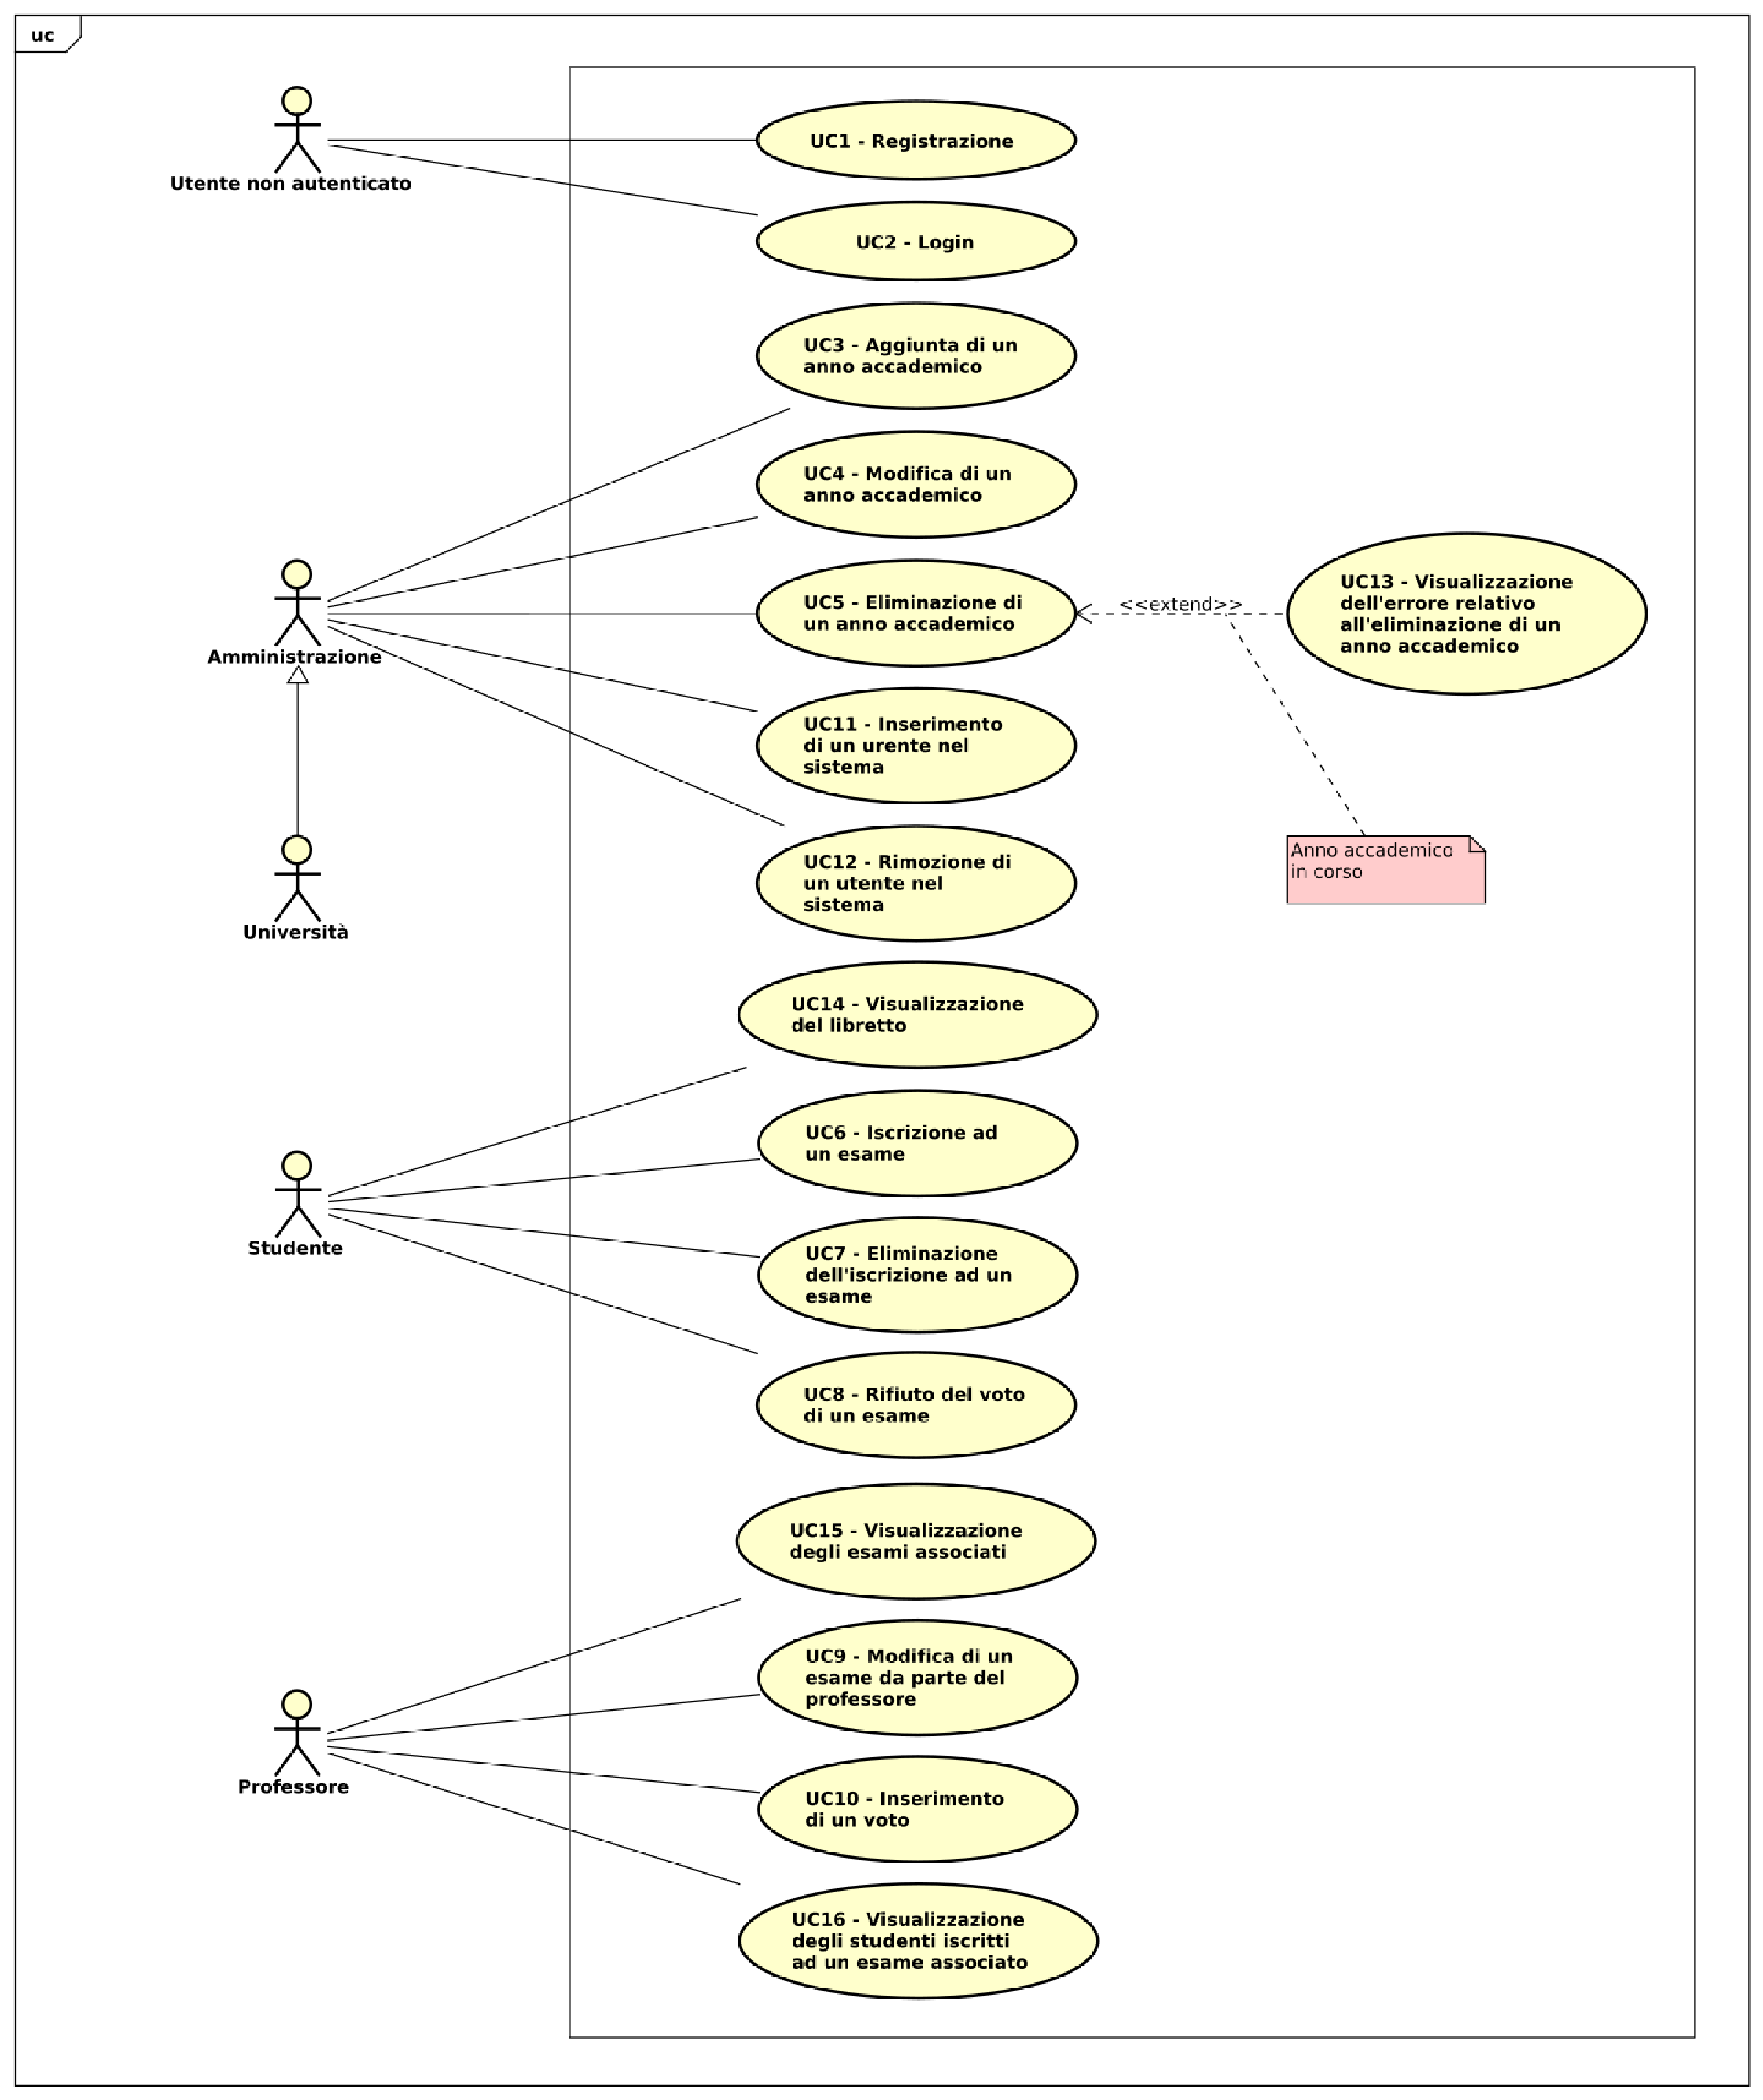
\includegraphics[scale=0.4]{./img/UC0.pdf}
	\caption{Registrazione }\label{}
\end{figure}
\begin{itemize}
	\item \textbf{Attori}: Utente non autenticato, Amministratore, Università, Studente, Professore;
	\item \textbf{Descrizione}: Nella pagina principale un utente non autenticato può registrarsi se non possiede un account o se non ha un account Metamask valido, altrimenti viene loggato automaticamente.
	Un professore può vedere gli esami associati, modificare questi esami, inserire un voto e vedere gli studenti iscritti ai suoi esami.
	Uno studente può: vedere il proprio libretto, iscriversi ad un esame, togliere l'iscrizione ad un esame e rifiutare un voto.
	L'amministratore e l'Università invece possono: aggiungere, modificare ed eliminare un anno accademico e inserire o rimuovere un utente dal sistema;
	\item \textbf{Precondizione}: Il sistema è avviato e mostra la pagina principale dell'applicazione;
	\item \textbf{Flusso principale degli eventi}: 
	\begin{itemize}
		\item L'utente non autenticato può registrarsi (UC1);
		\item L'utente non autenticato può loggarsi (UC2);
		\item L'amministrazione e l'università possono aggiungere un anno accademico (UC3);
		\item L'amministrazione e l'università possono modificare un anno accademico (UC4);
		\item L'amministrazione e l'università possono eliminare un anno accademico (UC5);
		\item L'amministrazione e l'università possono inserire un utente nel sistema (UC11);
		\item L'amministrazione e l'università possono rimuovere un utente dal sistema (UC12);
		\item Lo studente può visualizzare il libretto (UC14);
		\item Lo studente può iscriversi ad un esame (UC6);
		\item Lo studente può eliminare l'iscrizione ad un esame (UC7);
		\item Lo studente può rifiutare il voto di un esame (UC8);
		\item Il professore può visualizzare gli esami associati(UC15);
		\item Il professore può modificare un esame (UC9);
		\item Il professore può inserire un voto (UC10);
		\item Il professore puòVisualizzare gli studenti iscritti ad un esame (UC16).
	\end{itemize}
	\item \textbf{Postcondizione}: Il sistema ha ricevuto tutte le informazioni dall’utente sulle operazioni che vuole eseguire;
	\item \textbf{Estensioni}:
	\begin{itemize}
		\item Visualizzazione dell'errore relativo all'eliminazione di un anno accademico(UC13).
	\end{itemize}
\end{itemize}
\subsection{Caso d'uso \texorpdfstring{UC1}{UC1}: Registrazione }
\begin{figure} [H]
	\centering
	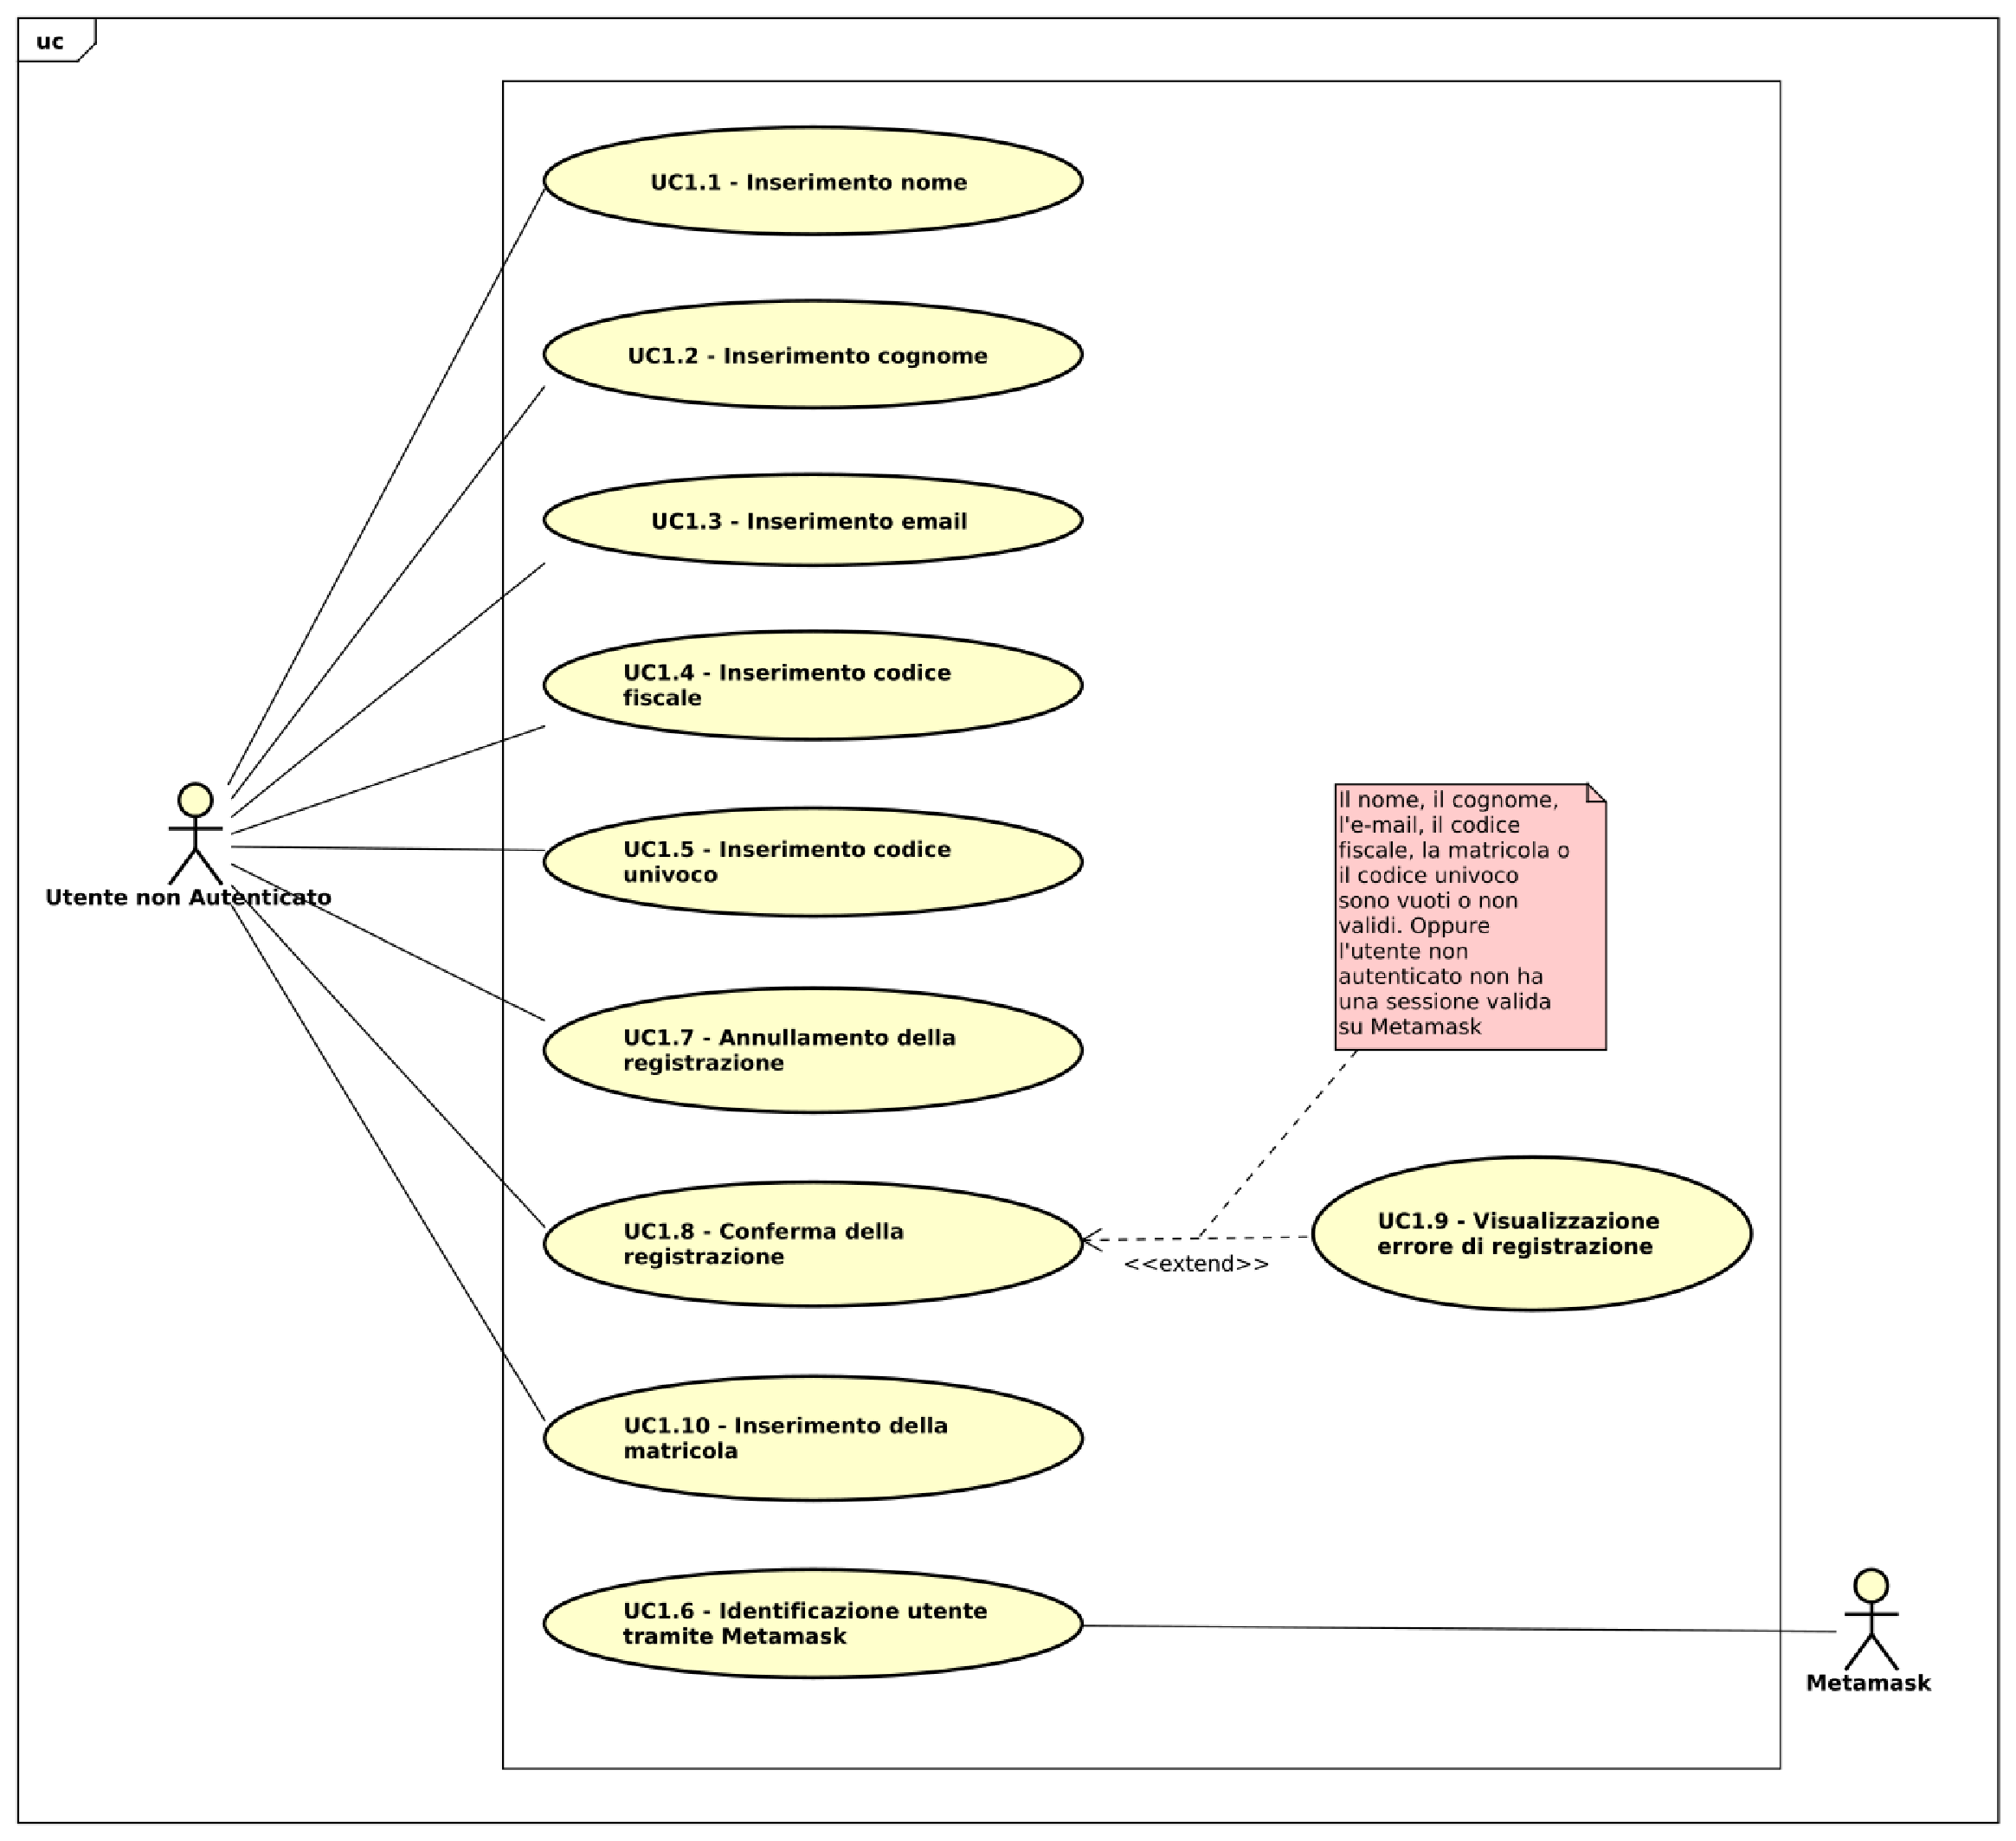
\includegraphics[scale=0.45]{./img/UC1.pdf}
	\caption{Registrazione }\label{}
\end{figure}
\begin{itemize}
	\item \textbf{Attori}: \emph{Metamask}\ped{G}, Utente non autenticato;
	\item \textbf{Descrizione}: Per accedere al sistema è necessario possedere un account;
	\item \textbf{Precondizione}: L'attore non possiede una account per accedere al sistema;
	\item \textbf{Flusso principale degli eventi}: L'attore si registra nel sistema attraverso i seguenti punti;
	\begin{itemize}
		\item Inserimento del nome (UC1.1);
		\item Inserimento del cognome (UC1.2);
		\item Inserimento della e-mail (UC1.3);
		\item Inserimento del codice fiscale (UC1.4);
		\item Inserimento del codice univoco (UC1.5);
		\item Identificazione utente tramite Metamask (UC1.6);
		\item Annullamento della registrazione (UC1.7);
		\item Conferma della registrazione (UC1.8);
		\item Visualizzazione dell'errore di registrazione (UC1.9);
		\item Inserimento della matricola (UC1.10).
	\end{itemize}
	\item \textbf{Postcondizione}: È stato creato un account per accedere al sistema.
\end{itemize}
\subsection{Caso d'uso \texorpdfstring{UC1.1}{UC1.1}: Inserimento del nome}
\begin{itemize}
	\item \textbf{Attori}: Utente non autenticato;
	\item \textbf{Descrizione}: L'attore deve inserire il proprio nome per potersi registrare;
	\item \textbf{Precondizione}: Il sistema fa visualizzare il campo di inserimento del nome;
	\item \textbf{Flusso principale degli eventi}: L'attore inserisce il proprio nome per effettuare la registrazione;
	\item \textbf{Postcondizione}: È stato inserito il nome dell'attore nel campo opportuno.
\end{itemize}
\subsection{Caso d'uso \texorpdfstring{UC1.2}{UC1.2}: Inserimento del cognome}
\begin{itemize}
	\item \textbf{Attori}: Utente non autenticato;
	\item \textbf{Descrizione}: L'attore deve inserire il proprio cognome per potersi registrare;
	\item \textbf{Precondizione}: Il sistema fa visualizzare il campo di inserimento del cognome;
	\item \textbf{Flusso principale degli eventi}: L'attore deve inserire il cognome per potersi registrare;
	\item \textbf{Postcondizione}: È stato inserito il cognome dell'attore nel campo opportuno.
\end{itemize}
\subsection{Caso d'uso \texorpdfstring{UC1.3}{UC1.3}: Inserimento della e-mail}
\begin{itemize}
	\item \textbf{Attori}: Utente non autenticato;
	\item \textbf{Descrizione}: L'attore deve inserire la proprio e-mail per potersi registrare;
	\item \textbf{Precondizione}: Il sistema fa visualizzare il campo di inserimento dell'e-mail;
	\item \textbf{Flusso principale degli eventi}: L'attore inserisce la propria e-mail per effettuare la registrazione;
	\item \textbf{Postcondizione}: È stata inserita la e-mail dell'attore nel campo opportuno.
\end{itemize}
\subsection{Caso d'uso \texorpdfstring{UC1.4}{UC1.4}: Inserimento del codice fiscale}
\begin{itemize}
	\item \textbf{Attori}: Utente non autenticato;
	\item \textbf{Descrizione}: L'attore deve inserire il proprio codice fiscale per potersi registrare;
	\item \textbf{Precondizione}: Il sistema fa visualizzare il campo di inserimento del codice fiscale;
	\item \textbf{Flusso principale degli eventi}: L'attore inserisce il proprio codice fiscale per effettuare la registrazione;
	\item \textbf{Postcondizione}: È stato inserito il codice fiscale dell'attore nel campo opportuno.
\end{itemize}
\subsection{Caso d'uso \texorpdfstring{UC1.5}{UC1.5}: Inserimento del codice univoco}
\begin{itemize}
	\item \textbf{Attori}: Utente non autenticato;
	\item \textbf{Descrizione}: L'attore inserisce il codice univoco rilasciato dall'università per la registrazione;
	\item \textbf{Precondizione}: Il sistema fa visualizzare il campo di inserimento del codice univoco;
	\item \textbf{Flusso principale degli eventi}: L'attore inserisce il codice univoco per effettuare la registrazione;
	\item \textbf{Postcondizione}: È stato inserito il codice univoco dell'attore nel campo opportuno.
\end{itemize}
\subsection{Caso d'uso \texorpdfstring{UC1.6}{UC1.6}: Identificazione utente tramite Metamask}
\begin{itemize}
	\item \textbf{Attori}: Metamask;
	\item \textbf{Descrizione}: Il sistema sfrutta l'interfaccia Metamask per poter identificare univocamente l'utente;
	\item \textbf{Precondizione}: Il sistema fa visualizzare la pagina di registrazione utente;
	\item \textbf{Flusso principale degli eventi}: Il sistema ha bisogno dell'interfaccia Metamask per poter registrare un utente;
	\item \textbf{Postcondizione}: Il sistema ha identificato l'utente.
\end{itemize}
\subsection{Caso d'uso \texorpdfstring{UC1.7}{UC1.7}: Annullamento della registrazione}
\begin{itemize}
	\item \textbf{Attori}: Utente non autenticato;
	\item \textbf{Descrizione}: L'attore decide di annullare la registrazione in corso;
	\item \textbf{Precondizione}: Il sistema fa visualizzare la pagina di registrazione;
	\item \textbf{Flusso principale degli eventi}: L'attore decide di annullare la registrazione in corso;
	\item \textbf{Postcondizione}: Il sistema non registra più l'attore in quanto esso ha annullato l'operazione.
\end{itemize}
\subsection{Caso d'uso \texorpdfstring{UC1.8}{UC1.8}: Conferma della registrazione}
\begin{itemize}
	\item \textbf{Attori}: Utente non autenticato;
	\item \textbf{Descrizione}: L'attore può aver inserito tutti i dati  e conferma la registrazione;
	\item \textbf{Precondizione}: Il sistema fa visualizzare la pagina di registrazione;
	\item \textbf{Flusso principale degli eventi}: L'attore dopo aver inserito i dati può completare la registrazione confermandola;
	\item \textbf{Postcondizione}: Il sistema registra l'attore in quanto esso ha confermato la registrazione.
	\item \textbf{Estensioni}:
	\begin{itemize}
		\item Visualizzazione dell'errore di registrazione (UC1.9).
	\end{itemize}
\end{itemize}
\subsection{Caso d'uso \texorpdfstring{UC1.9}{UC1.9}: Visualizzazione dell'errore di registrazione}
\begin{itemize}
	\item \textbf{Attori}: Utente non autenticato;
	\item \textbf{Descrizione}: L'attore può visualizzare un errore nel caso avessero inseriti dati errati;
	\item \textbf{Precondizione}: Il sistema ha ricevuto campi dati errati o vuoti;
	\item \textbf{Flusso principale degli eventi}: L'attore visualizza un messaggio d'errore relativo all'inserimento mancato o non valido di:
	\begin{itemize}
		\item Nome;
		\item Cognome;
		\item E-mail;
		\item Codice fiscale;
		\item Codice univoco;
		\item Matricola.
	\end{itemize}
	\item \textbf{Postcondizione}: Il sistema fa visualizzare un messaggio d'errore riguardante il tentativo di registrazione con campi dati errati o vuoti.
\end{itemize}
\subsection{Caso d'uso \texorpdfstring{UC1.10}{UC1.10}: Inserimento della matricola}
\begin{itemize}
	\item \textbf{Attori}: Utente non autenticato;
	\item \textbf{Descrizione}: L'attore inserisce la matricola ad esso associata dall'università per la registrazione;
	\item \textbf{Precondizione}: Il sistema fa visualizzare il campo di inserimento della matricola;
	\item \textbf{Flusso principale degli eventi}: L'attore inserisce la matricola per effettuare la registrazione;
	\item \textbf{Postcondizione}: È stata inserita la matricola dell'attore nel campo opportuno.
\end{itemize}
\subsection{Caso d'uso \texorpdfstring{UC2}{UC2}: Login}
\begin{figure} [H]
	\centering
	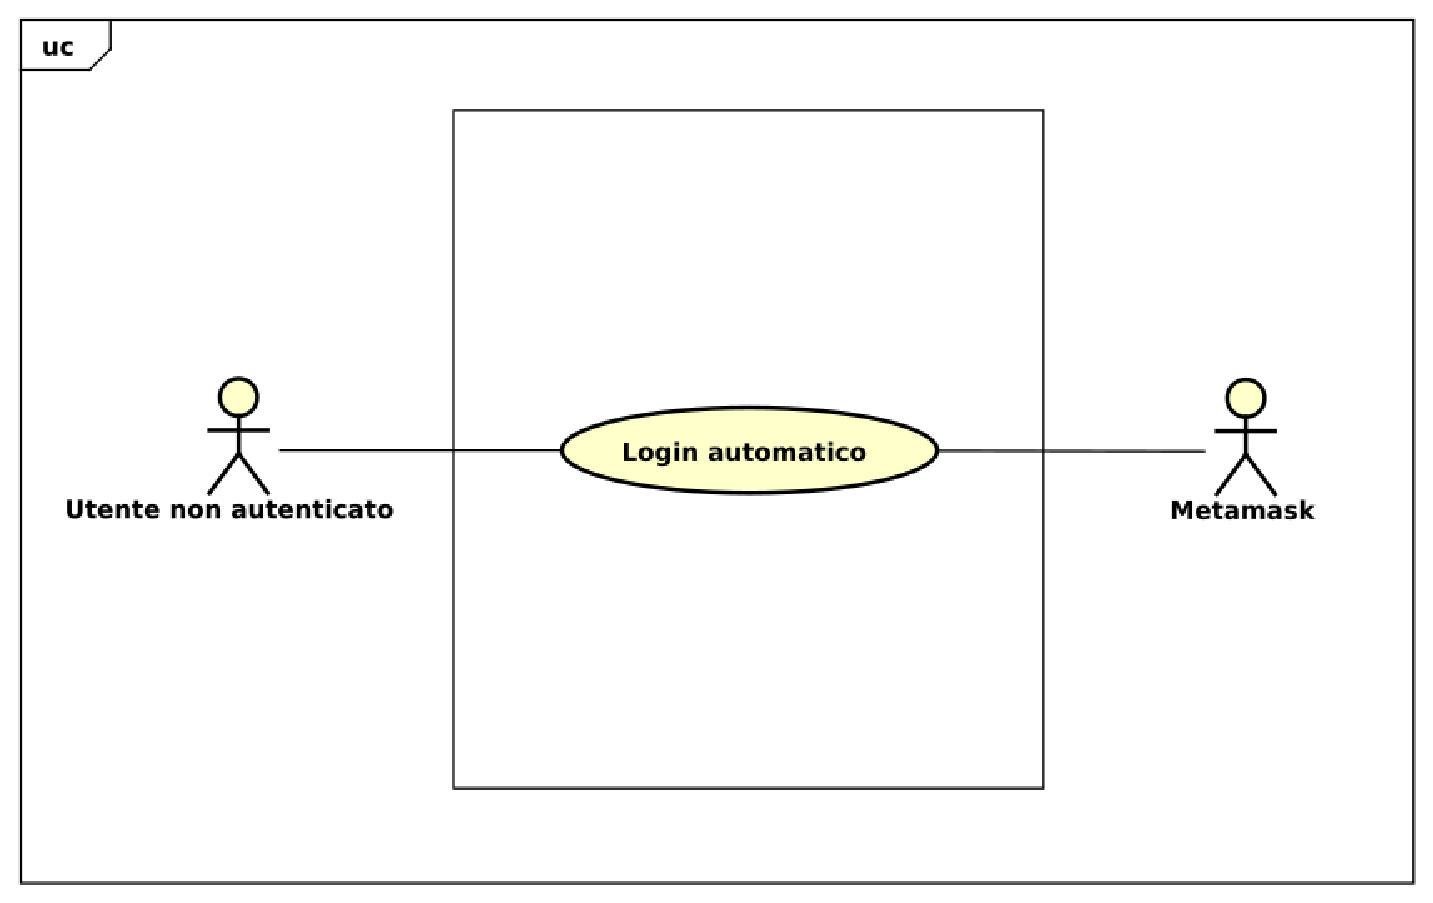
\includegraphics[scale=0.45]{./img/UC2.pdf}
	\caption{Login}\label{}
\end{figure}
\begin{itemize}
	\item \textbf{Attori}: Utente non autenticato;
	\item \textbf{Descrizione}: Il sistema è avviato ma è necessario loggarsi per accedervi;
	\item \textbf{Precondizione}: Il sistema non permette l'accesso all'attore non loggato;
	\item \textbf{Flusso principale degli eventi}: L'attore effettua automaticamente il login attuando:
	\begin{itemize}
		\item Login automatico (UC2.1).
	\end{itemize}
	\item \textbf{Postcondizione}: Il sistema permette l'accesso all'attore che adesso è loggato.
\end{itemize}
\subsection{Caso d'uso \texorpdfstring{UC2.1}{UC2.1}: Login automatico}
\begin{itemize}
	\item \textbf{Attori}: Metamask, Utente non autenticato;
	\item \textbf{Descrizione}: Il sistema logga automaticamente l'attore se ha metamask attivo e la sua \emph{chiave pubblica}\ped{G} coincide con una presente all'interno del sistema;
	\item \textbf{Precondizione}: Il sistema non riconosce l'attore;
	\item \textbf{Flusso principale degli eventi}: L'attore con Metamask attivo e precedentemente registrato, entra nel sistema senza compiere alcuna azione;
	\item \textbf{Postcondizione}: Il sistema riconosce l'attore.
\end{itemize}
\subsection{Caso d'uso \texorpdfstring{UC3}{UC3}: Aggiunta di un anno accademico}
\begin{figure} [H]
	\centering
	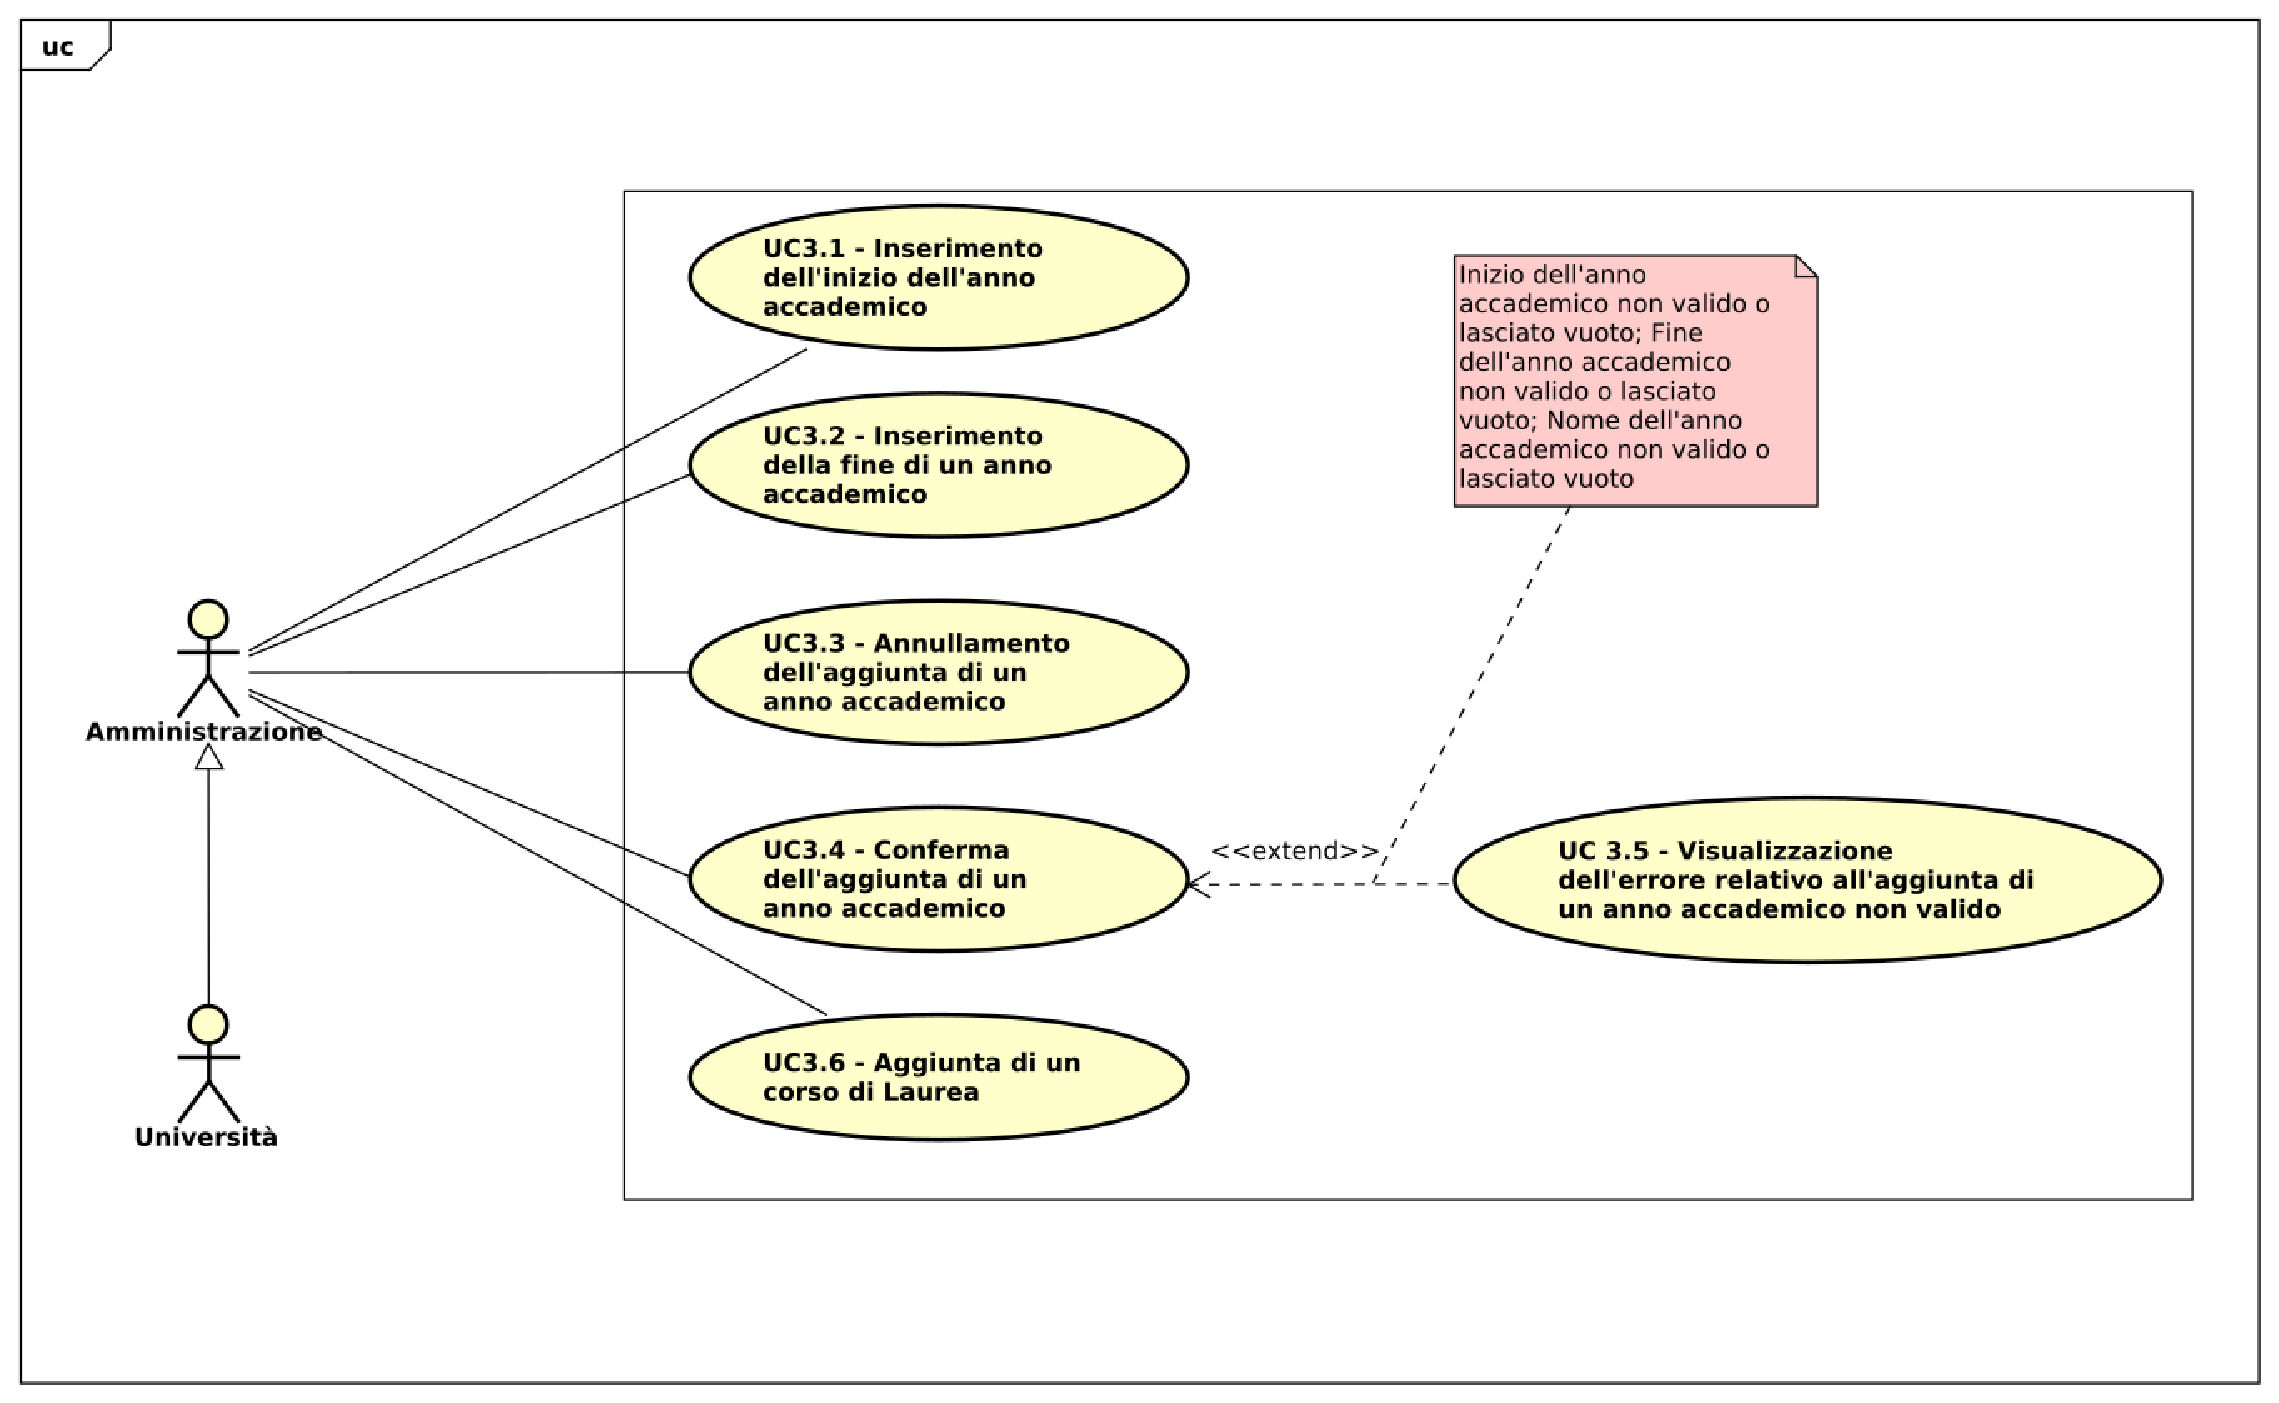
\includegraphics[scale=0.45]{./img/UC3.pdf}
	\caption{Aggiunta di un anno accademico}\label{}
\end{figure}
\begin{itemize}
	\item \textbf{Attori}: Amministratore, Università;
	\item \textbf{Descrizione}: L'attore aggiunge un anno accademico alla lista degli anni accademici;
	\item \textbf{Precondizione}: La lista degli anni accademici è vuota oppure non contiene l'anno accademico che l'attore vuole inserire;
	\item \textbf{Flusso principale degli eventi}: L'attore, per inserire l'anno accademico alla lista, deve seguire i seguenti punti:
	\begin{itemize}
		\item Inserimento dell'inizio di un accademico (UC3.1);
		\item Inserimento della fine di un accademico (UC3.2);
		\item Annullamento dell'aggiunta di un anno accademico (UC3.3);
		\item Conferma dell'aggiunta di un anno accademico (UC3.4);
		\item Visualizzazione dell'errore relativo all'aggiunta di un anno accademico non valido (UC3.5);
		\item Aggiunta di un corso di laurea (UC3.6).
	\end{itemize}
	\item \textbf{Postcondizione}: Il sistema può aver compilato dei campi relativi all'aggiunta di un nuovo anno accademico.
\end{itemize}
\subsection{Caso d'uso \texorpdfstring{UC3.1}{UC3.1}: Inserimento dell'inizio di un accademico}
\begin{itemize}
	\item \textbf{Attori}: Amministratore, Università;
	\item \textbf{Descrizione}: L'attore compila il campo relativo all'inizio dell'anno accademico;
	\item \textbf{Precondizione}: Il sistema fa visualizzare il campo di inserimento dell'inizio dell'anno accademico;
	\item \textbf{Flusso principale degli eventi}: L'attore imposta l'inizio dell'anno accademico;
	\item \textbf{Postcondizione}: È stato inserito l'inizio dell'anno accademico nel campo opportuno.
\end{itemize}
\subsection{Caso d'uso \texorpdfstring{UC3.2}{UC3.2}: Inserimento della fine di un accademico}
\begin{itemize}
	\item \textbf{Attori}: Amministratore, Università;
	\item \textbf{Descrizione}: L'attore compila il campo relativo alla fine dell'anno accademico;
	\item \textbf{Precondizione}: Il sistema fa visualizzare il campo di inserimento della fine dell'anno accademico;
	\item \textbf{Flusso principale degli eventi}: L'attore imposta la fine dell'anno accademico;
	\item \textbf{Postcondizione}: È stata inserita la fine dell'anno accademico nel campo opportuno.
\end{itemize}
\subsection{Caso d'uso \texorpdfstring{UC3.3}{UC3.3}: Annullamento dell'aggiunta di un anno accademico}
\begin{itemize}
	\item \textbf{Attori}: Amministratore, Università;
	\item \textbf{Descrizione}: L'attore può voler più aggiungere un anno accademico alla lista degli anni accademici;
	\item \textbf{Precondizione}: Il sistema fa visualizzare la pagina relativa all'aggiunta di un anno accademico;
	\item \textbf{Flusso principale degli eventi}: L'attore non inserisce più un anno accademico e quindi annulla l'operazione;
	\item \textbf{Postcondizione}: Il sistema non aggiunge più un anno accademico in quanto l'attore ha annullato l'operazione.
\end{itemize}
\subsection{Caso d'uso \texorpdfstring{UC3.4}{UC3.4}: Conferma dell'aggiunta di un anno accademico}
\begin{itemize}
	\item \textbf{Attori}: Amministratore, Università;
	\item \textbf{Descrizione}: L'attore conferma l'aggiunta di un anno accademico alla lista degli anni accademici;
	\item \textbf{Precondizione}: Il sistema fa visualizzare la pagina relativa all'aggiunta di un anno accademico;
	\item \textbf{Flusso principale degli eventi}: L'attore, confermando l'inserimento dei dati, aggiunge un anno accademico alla lista degli anni accademici;
	\item \textbf{Postcondizione}: Il sistema aggiunge un anno accademico in quanto l'attore ha confermato l'operazione;
	\item \textbf{Estensioni}:
	\begin{itemize}
		\item Visualizzazione dell'errore relativo all'aggiunta di un anno accademico non valido (UC3.5).
	\end{itemize}
\end{itemize}
\subsection{Caso d'uso \texorpdfstring{UC3.5}{UC3.5}: Visualizzazione dell'errore relativo all'aggiunta di un anno accademico non valido}
\begin{itemize}
	\item \textbf{Attori}: Amministratore, Università;
	\item \textbf{Descrizione}: L'attore aggiunge i dettagli di un anno accademico senza rispettarne la validazione;
	\item \textbf{Precondizione}: Il sistema ha ricevuto campi dati errati o vuoti;
	\item \textbf{Flusso principale degli eventi}: L'attore, impostando in maniera errata i campi dell'anno accademico, può visualizzare uno dei seguenti errori:
	\begin{itemize}
		\item Inizio dell'anno accademico non valido o lasciato vuoto;
		\item Fine dell'anno accademico non valido o lasciato vuoto;
		\item Nome dell'anno accademico non valido o lasciato vuoto.
	\end{itemize}
	\item \textbf{Postcondizione}: Il sistema fa visualizzare un messaggio d'errore riguardante il tentativo di aggiungere un anno accademico con campi dati errati o vuoti.
\end{itemize}
\subsection{Caso d'uso \texorpdfstring{UC3.6}{UC3.6}: Aggiunta di un corso di laurea}
\begin{figure} [H]
	\centering
	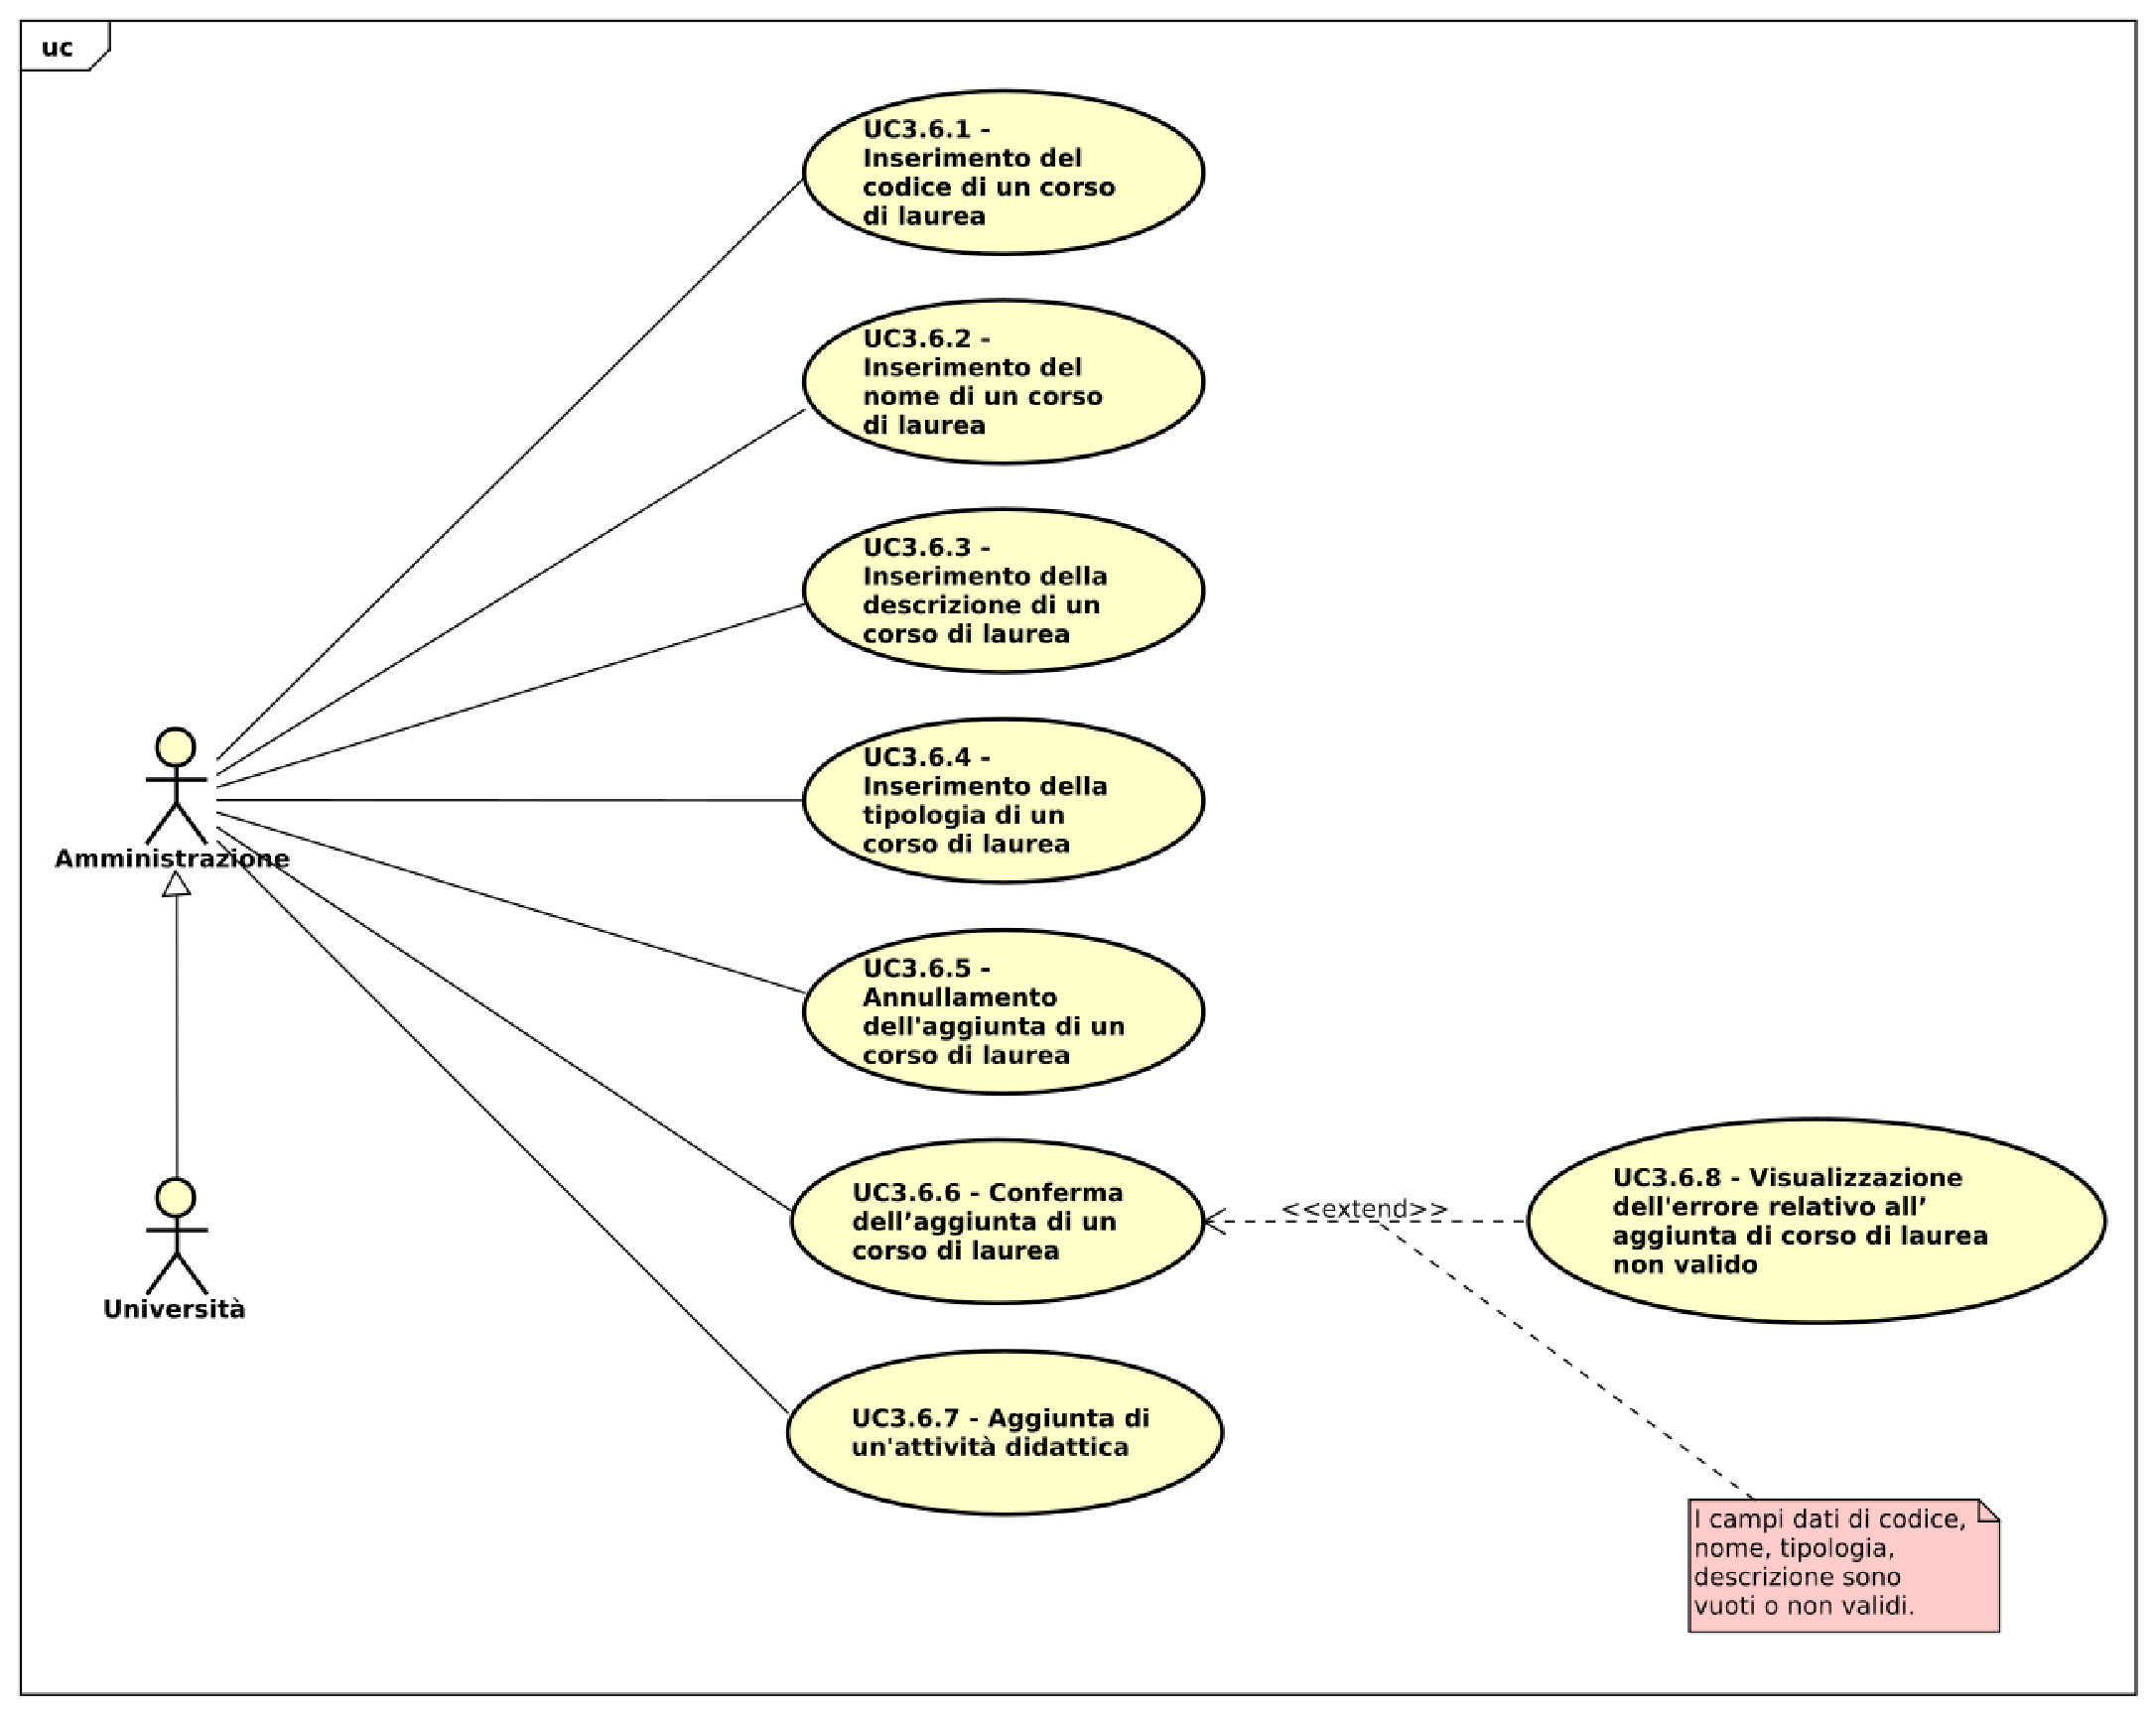
\includegraphics[scale=0.45]{./img/UC3-6.pdf}
	\caption{Aggiunta di un corso di laurea}\label{}
\end{figure}
\begin{itemize}
	\item \textbf{Attori}: Amministratore, Università;
	\item \textbf{Descrizione}: L'attore aggiunge un corso di laurea alla lista dei corsi di laurea;
	\item \textbf{Precondizione}: La lista dei corsi di laurea è vuota oppure non contiene il corso di laurea che l'attore vuole inserire;
	\item \textbf{Flusso principale degli eventi}: L'attore, per inserire il corso di laurea alla lista, deve seguire i seguenti punti:
	\begin{itemize}
		\item Inserimento del codice di un corso di laurea (UC3.6.1);
		\item Inserimento del nome di un corso di laurea (UC3.6.2);
		\item Inserimento della descrizione di un corso di laurea (UC3.6.3);
		\item Inserimento della tipologia di un corso di laurea (UC3.6.4);
		\item Annullamento dell'aggiunta di un corso di laurea (UC3.6.5);
		\item Conferma dell’aggiunta di un corso di laurea (UC3.6.6);
		\item Aggiunta di un'attività didattica (UC3.6.7);
		\item Visualizzazione dell'errore relativo all’aggiunta di corso di laurea non valido (UC3.6.8).
	\end{itemize}
	\item \textbf{Postcondizione}: Il sistema può aver compilato dei campi relativi all'aggiunta di un nuovo corso di laurea.
\end{itemize}
\subsection{Caso d'uso \texorpdfstring{UC3.6.1}{UC3.6.1}: Inserimento del codice di un corso di laurea}
\begin{itemize}
	\item \textbf{Attori}: Amministratore, Università;
	\item \textbf{Descrizione}: L'attore compila il campo relativo al codice del corso di laurea;
	\item \textbf{Precondizione}: Il sistema fa visualizzare il campo di inserimento del codice di un corso di laurea;
	\item \textbf{Flusso principale degli eventi}: L'attore imposta il codice del corso di laurea;
	\item \textbf{Postcondizione}: È stato inserito il codice del corso di laurea nel campo opportuno.
\end{itemize}
\subsection{Caso d'uso \texorpdfstring{UC3.6.2}{UC3.6.2}: Inserimento del nome di un corso di laurea}
\begin{itemize}
	\item \textbf{Attori}: Amministratore, Università;
	\item \textbf{Descrizione}: L'attore compila il campo relativo al nome del corso di laurea;
	\item \textbf{Precondizione}: Il sistema fa visualizzare il campo di inserimento del nome di un corso di laurea;
	\item \textbf{Flusso principale degli eventi}: L'attore imposta il nome del corso di laurea;
	\item \textbf{Postcondizione}: È stato inserito il nome del corso di laurea nel campo opportuno.
\end{itemize}
\subsection{Caso d'uso \texorpdfstring{UC3.6.3}{UC3.6.3}: Inserimento della descrizione di un corso di laurea}
\begin{itemize}
	\item \textbf{Attori}: Amministratore, Università;
	\item \textbf{Descrizione}: L'attore compila il campo relativo alla descrizione del corso di laurea;
	\item \textbf{Precondizione}: Il sistema fa visualizzare il campo di inserimento della descrizione di un corso di laurea;
	
	\item \textbf{Flusso principale degli eventi}: L'attore aggiunge la descrizione del corso di laurea;
	\item \textbf{Postcondizione}: È stata inserita la descrizione del corso di laurea nel campo opportuno.
\end{itemize}
\subsection{Caso d'uso \texorpdfstring{UC3.6.4}{UC3.6.4}: Inserimento della tipologia di un corso di laurea}
\begin{itemize}
	\item \textbf{Attori}: Amministratore, Università;
	\item \textbf{Descrizione}: L'attore compila il campo relativo alla tipologia del corso di laurea;
	\item \textbf{Precondizione}: Il sistema fa visualizzare il campo di inserimento della tipologia di un corso di laurea;
	\item \textbf{Flusso principale degli eventi}: L'attore aggiunge la tipologia del corso di laurea;
	\item \textbf{Postcondizione}: È stata inserita la tipologia del corso di laurea nel campo opportuno.
\end{itemize}
\subsection{Caso d'uso \texorpdfstring{UC3.6.5}{UC3.6.5}: Annullamento dell'aggiunta di un corso di laurea}
\begin{itemize}
	\item \textbf{Attori}: Amministratore, Università;
	\item \textbf{Descrizione}: L'attore non aggiunge più un corso di laurea alla lista dei corsi di laurea;
	
	\item \textbf{Precondizione}: l sistema fa visualizzare la pagina relativa all'aggiunta di un corso di laurea;
	
	\item \textbf{Flusso principale degli eventi}: L'attore non inserisce più un corso di laurea e quindi annulla l'operazione;
	
	\item \textbf{Postcondizione}: Il sistema non aggiunge più un corso di laurea in quanto l'attore ha annullato l'operazione.
	
\end{itemize}
\subsection{Caso d'uso \texorpdfstring{UC3.6.6}{UC3.6.6}: Conferma dell’aggiunta di un corso di laurea}
\begin{itemize}
	\item \textbf{Attori}: Amministratore, Università;
	\item \textbf{Descrizione}: L'attore conferma l'aggiunta di corso di laurea alla lista dei corsi di laurea;
	
	\item \textbf{Precondizione}: Il sistema fa visualizzare la pagina relativa all'aggiunta di un corso di laurea;
	
	\item \textbf{Flusso principale degli eventi}: L'attore, confermando l'inserimento dei dati, aggiunge un corso di laurea alla lista dei corsi di laurea;
	
	\item \textbf{Postcondizione}: Il sistema aggiunge un corso di laurea in quanto l'attore ha confermato l'operazione;
	
	\item \textbf{Estensioni}:
	\begin{itemize}
		\item Visualizzazione dell'errore relativo all’aggiunta di corso di laurea non valido (UC3.6.8).
	\end{itemize}
\end{itemize}
\subsection{Caso d'uso \texorpdfstring{UC3.6.7}{UC3.6.7}: Aggiunta di un'attività didattica}
\begin{figure} [H]
	\centering
	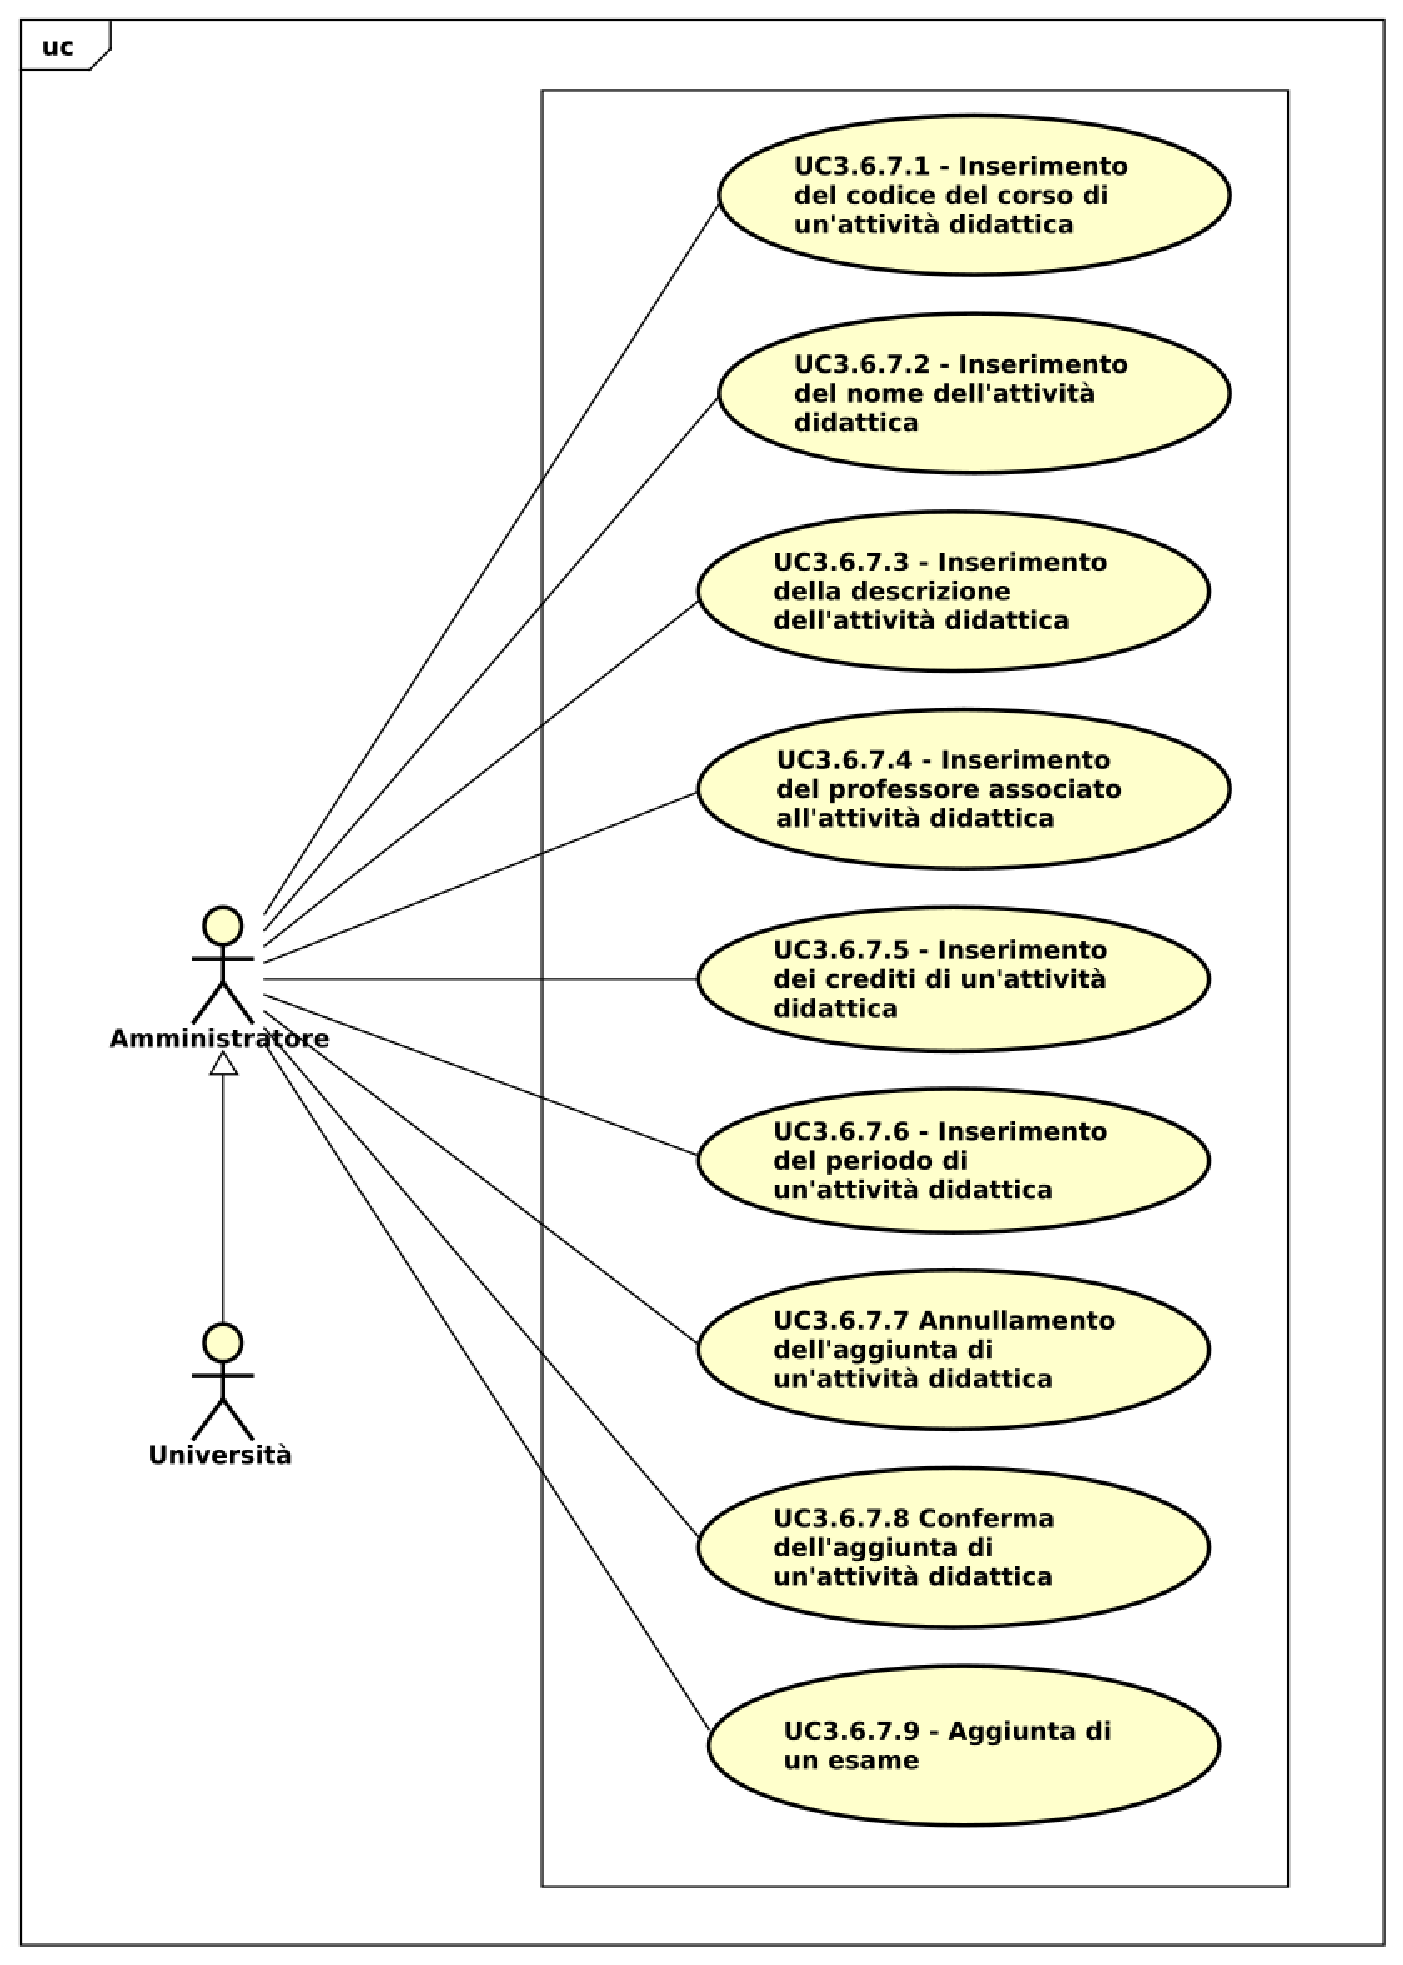
\includegraphics[scale=0.45]{./img/UC3-6-7.pdf}
	\caption{Aggiunta di un'attività didattica}\label{}
\end{figure}
\begin{itemize}
	\item \textbf{Attori}: Amministratore, Università;
	\item \textbf{Descrizione}: L'attore aggiunge un'attività didattica alla lista delle attività didattiche;
	
	\item \textbf{Precondizione}: La lista delle attività didattiche è vuota oppure non contiene l'attività didattica che l'attore vuole inserire;
	
	\item \textbf{Flusso principale degli eventi}: L'attore, per inserire l'attività didattica alla lista, deve seguire i seguenti punti:
	
	\begin{itemize}
		\item Inserimento del codice del corso di un'attività didattica (UC3.6.7.1);
		\item Inserimento del nome di un’attività didattica (UC3.6.7.2);
		\item Inserimento della descrizione di un'attività didattica (UC3.6.7.3);
		\item Inserimento del professore associato ad un'attività didattica (UC3.6.7.4);
		\item Inserimento dei crediti di un’attività didattica (UC3.6.7.5);
		\item Inserimento del periodo di un’attività didattica (UC3.6.7.6);
		\item Annullamento dell’aggiunta di un’attività didattica (UC3.6.7.7);
		\item Conferma dell’aggiunta di un’attività didattica (UC3.6.7.8);
		\item Aggiunta di un esame (UC3.6.7.9);
		\item Visualizzazione dell'errore relativo all’aggiunta di un’attività didattica non valida (UC3.6.7.10).
	\end{itemize}
	\item \textbf{Postcondizione}: Il sistema può aver compilato dei campi relativi all'aggiunta di una nuova attività didattica.
	
\end{itemize}
\subsection{Caso d'uso \texorpdfstring{UC3.6.7.1}{UC3.6.7.1}: Inserimento del codice del corso di un'attività didattica}
\begin{itemize}
	\item \textbf{Attori}: Amministratore, Università;
	\item \textbf{Descrizione}: L'attore compila il campo relativo al codice del corso dell'attività didattica;
	
	\item \textbf{Precondizione}: Il sistema fa visualizzare il campo di inserimento del codice di un'attività didattica;
	
	\item \textbf{Flusso principale degli eventi}: L'attore imposta il codice del corso dell'attività didattica;
	
	\item \textbf{Postcondizione}: È stato inserito il codice dell'attività didattica nel campo opportuno.
	
\end{itemize}
\subsection{Caso d'uso \texorpdfstring{UC3.6.7.2}{UC3.6.7.2}: Inserimento del nome di un’attività didattica}
\begin{itemize}
	\item \textbf{Attori}: Amministratore, Università;
	\item \textbf{Descrizione}: L'attore compila il campo relativo al nome del corso dell'attività didattica;
	
	\item \textbf{Precondizione}: Il sistema fa visualizzare il campo di inserimento del nome di un'attività didattica;
	
	\item \textbf{Flusso principale degli eventi}: L'attore imposta il nome del corso dell'attività didattica;
	
	\item \textbf{Postcondizione}: È stato inserito il nome dell'attività didattica nel campo opportuno.
\end{itemize}
\subsection{Caso d'uso \texorpdfstring{UC3.6.7.3}{UC3.6.7.3}: Inserimento della descrizione di un'attività didattica}
\begin{itemize}
	\item \textbf{Attori}: Amministratore, Università;
	\item \textbf{Descrizione}: L'attore compila il campo relativo alla descrizione dell'attività didattica;
	
	\item \textbf{Precondizione}: Il sistema fa visualizzare il campo di inserimento della descrizione di un'attività didattica;
	
	\item \textbf{Flusso principale degli eventi}: L'attore imposta la descrizione dell'attività didattica;
	
	\item \textbf{Postcondizione}: È stata inserita la descrizione dell'attività didattica nel campo opportuno.
	
\end{itemize}
\subsection{Caso d'uso \texorpdfstring{UC3.6.7.4}{UC3.6.7.4}: Inserimento del professore associato ad un'attività didattica}
\begin{itemize}
	\item \textbf{Attori}: Amministratore, Università;
	\item \textbf{Descrizione}: L'attore compila il campo relativo al professore associato all'attività didattica;
	
	\item \textbf{Precondizione}: Il sistema fa visualizzare il campo di inserimento del professore associato ad un'attività didattica;
	\item \textbf{Flusso principale degli eventi}: L'attore imposta il professore associato all'attività didattica;
	
	\item \textbf{Postcondizione}: È stato inserito il professore associato all'attività didattica nel campo opportuno.
	
\end{itemize}
\subsection{Caso d'uso \texorpdfstring{UC3.6.7.5}{UC3.6.7.5}: Inserimento dei crediti di un’attività didattica}
\begin{itemize}
	\item \textbf{Attori}: Amministratore, Università;
	\item \textbf{Descrizione}: L'attore compila il campo relativo ai crediti dell'attività didattica;
	
	\item \textbf{Precondizione}: Il sistema fa visualizzare il campo di inserimento dei crediti di un'attività didattica;
	
	\item \textbf{Flusso principale degli eventi}: L'attore imposta i crediti dell'attività didattica;
	
	\item \textbf{Postcondizione}: Sono stati inseriti i crediti dell'attività didattica nel campo opportuno.
	
\end{itemize}
\subsection{Caso d'uso \texorpdfstring{UC3.6.7.6}{UC3.6.7.6}: Inserimento del periodo di un’attività didattica}
\begin{itemize}
	\item \textbf{Attori}: Amministratore, Università;
	\item \textbf{Descrizione}: L'attore compila il campo relativo al periodo dell'attività didattica;
	
	\item \textbf{Precondizione}: Il sistema fa visualizzare il campo di inserimento del periodo di un'attività didattica;
	
	\item \textbf{Flusso principale degli eventi}: L'attore imposta il periodo dell'attività didattica;
	
	\item \textbf{Postcondizione}: È stato inserito il periodo dell'attività didattica nel campo opportuno.
	
\end{itemize}
\subsection{Caso d'uso \texorpdfstring{UC3.6.7.7}{UC3.6.7.7}: Annullamento dell’aggiunta di un’attività didattica}
\begin{itemize}
	\item \textbf{Attori}: Amministratore, Università;
	\item \textbf{Descrizione}: L'attore non aggiunge più un'attività didattica alla lista delle attività didattiche;
	
	\item \textbf{Precondizione}: Il sistema fa visualizzare la pagina relativa all'aggiunta di un'attività didattica;
	
	\item \textbf{Flusso principale degli eventi}: L'attore non inserisce più un'attività didattica e quindi annulla l'operazione;
	
	\item \textbf{Postcondizione}: Il sistema non aggiunge più un'attività didattica in quanto l'attore ha annullato l'operazione.
\end{itemize}
\subsection{Caso d'uso \texorpdfstring{UC3.6.7.8}{UC3.6.7.8}: Conferma dell’aggiunta di un’attività didattica}
\begin{itemize}
	\item \textbf{Attori}: Amministratore, Università;
	\item \textbf{Descrizione}: L'attore conferma l'aggiunta di un’attività didattica alla lista delle attività didattiche;
	
	\item \textbf{Precondizione}: Il sistema fa visualizzare la pagina relativa all'aggiunta di un’attività didattica;
	
	\item \textbf{Flusso principale degli eventi}: L'attore, confermando l'inserimento dei dati, aggiunge un’attività didattica alla lista delle attività didattiche;
	
	\item \textbf{Postcondizione}: Il sistema aggiunge un'attività didattica in quanto l'attore ha confermato l'operazione;
	
	\item \textbf{Estensioni}:
	\begin{itemize}
		\item Visualizzazione dell'errore relativo all’aggiunta di un’attività didattica non valida (UC3.6.7.10).
	\end{itemize}
\end{itemize}
\subsection{Caso d'uso \texorpdfstring{UC3.6.7.9}{UC3.6.7.9}: Aggiunta di un esame}
\begin{figure} [H]
	\centering
	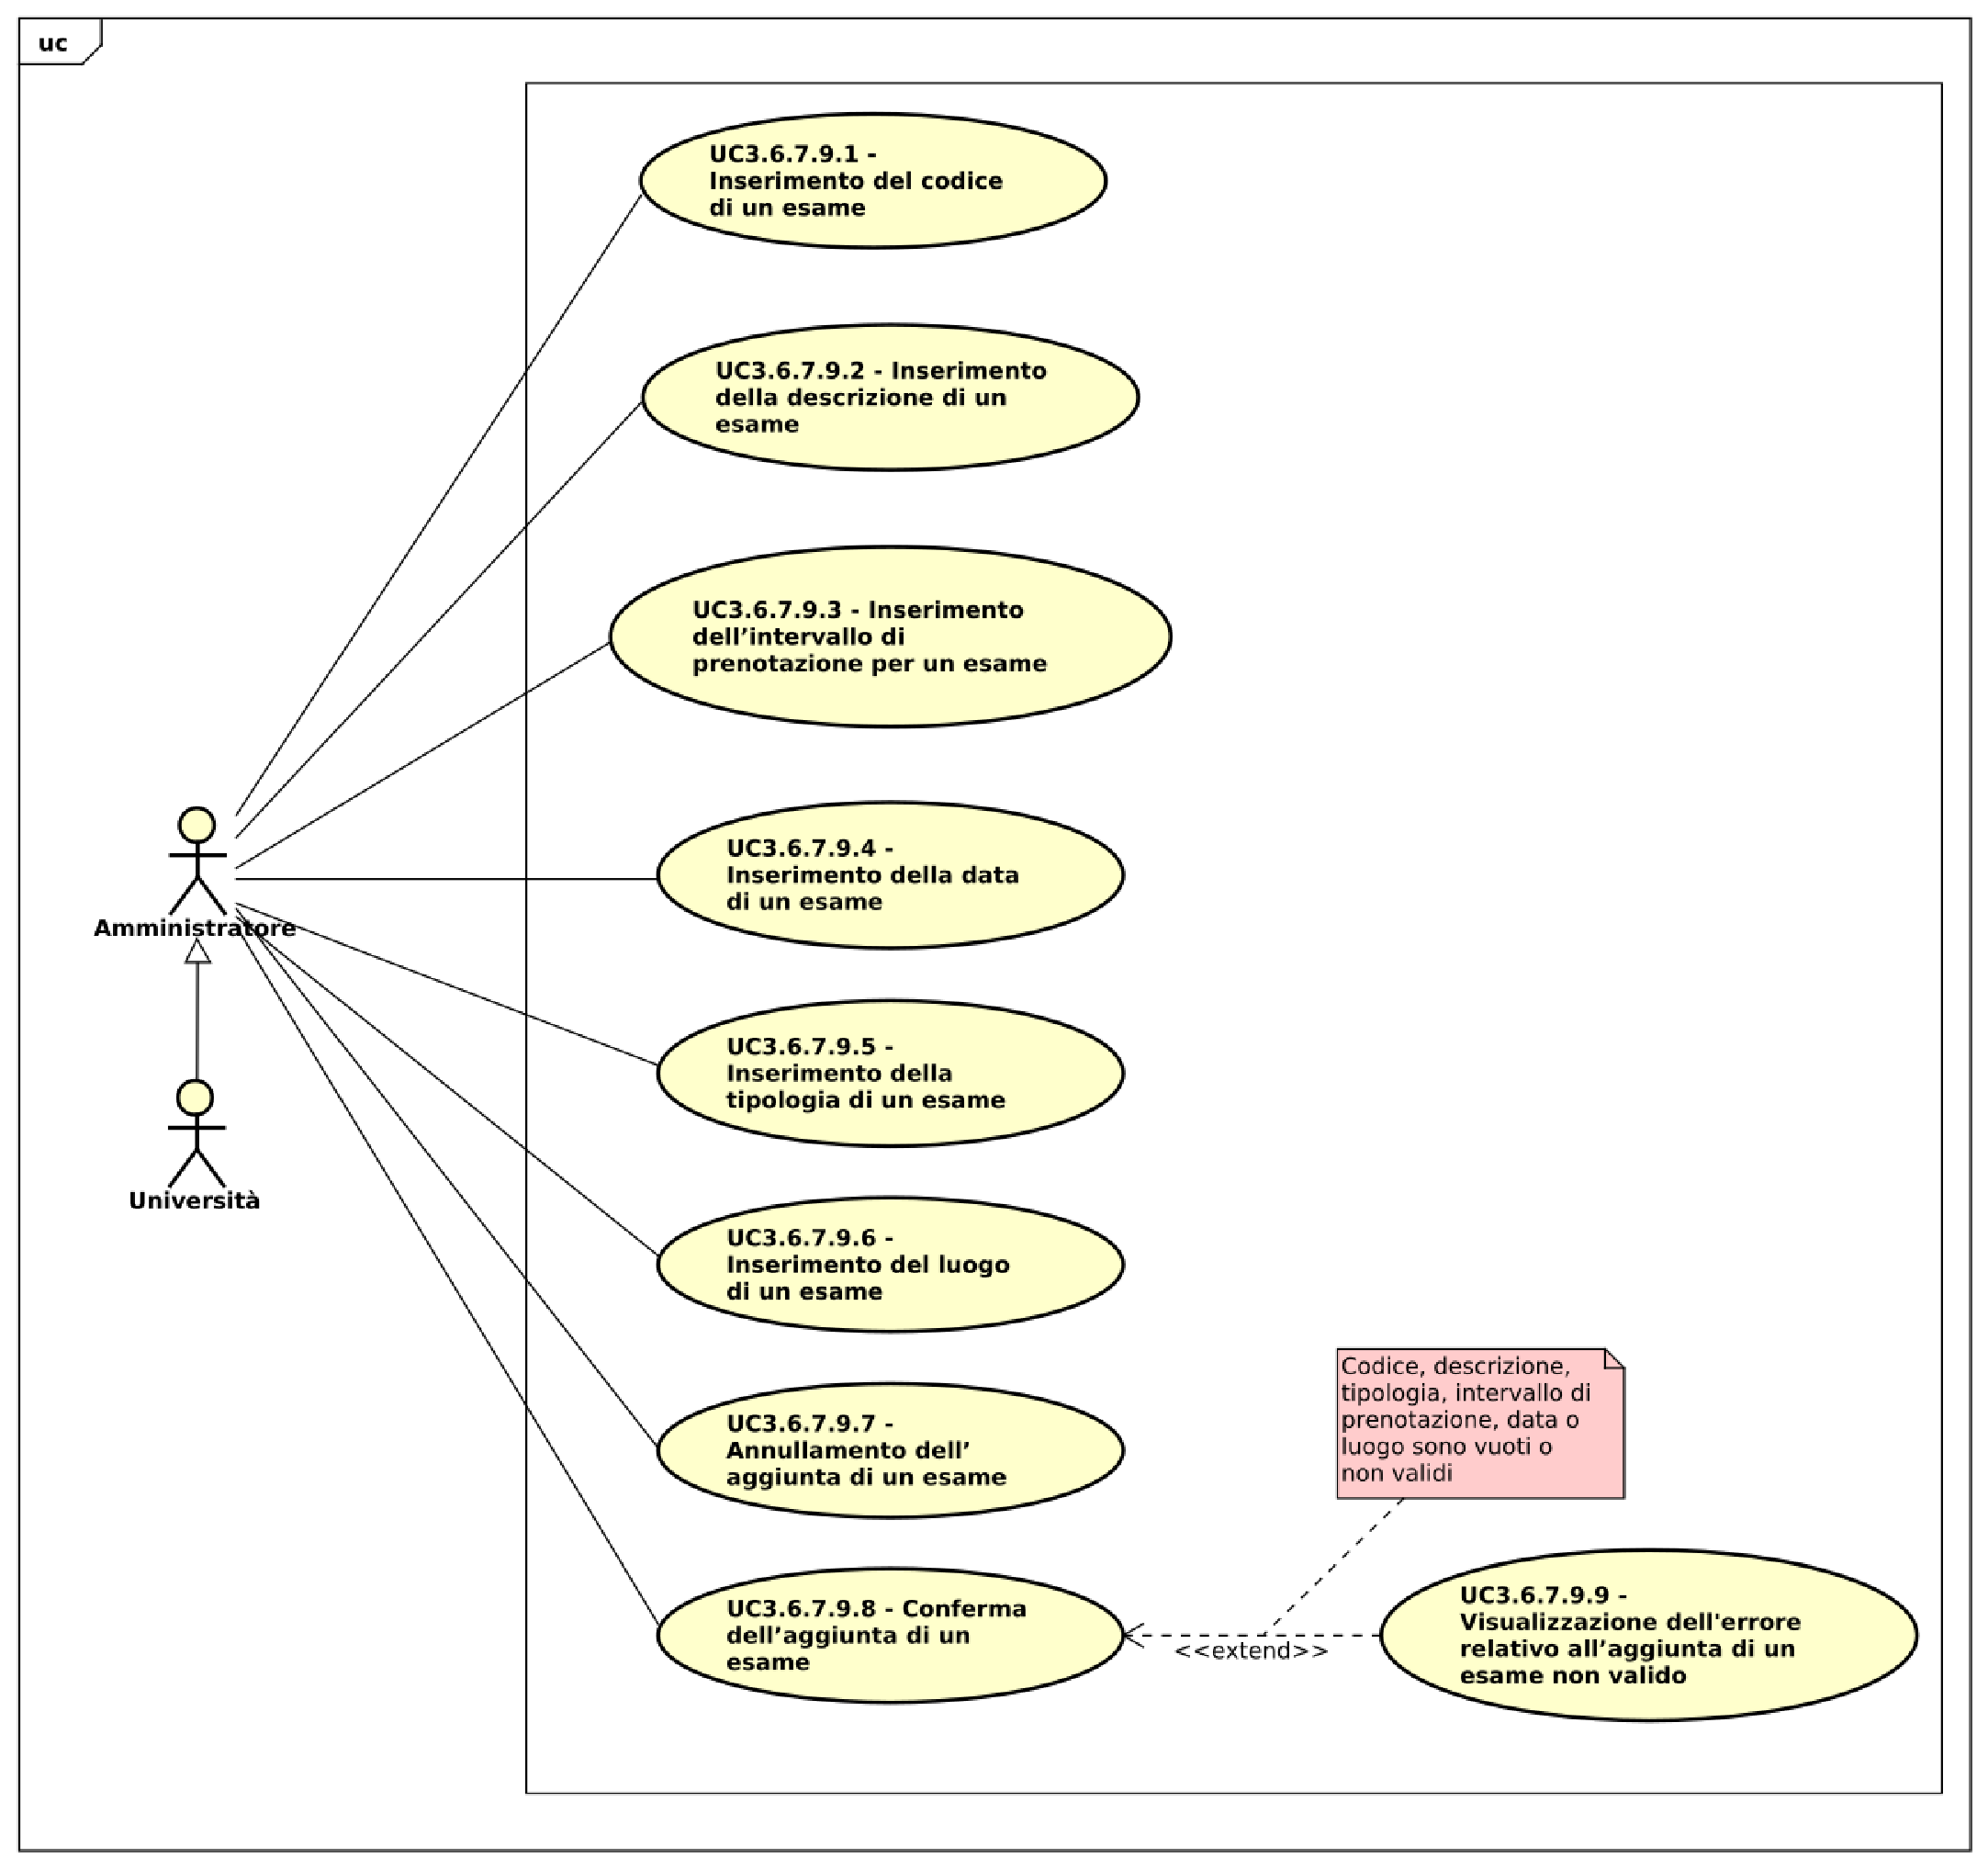
\includegraphics[scale=0.45]{./img/UC3-6-7-9.pdf}
	\caption{Aggiunta di un esame}\label{}
\end{figure}
\begin{itemize}
	\item \textbf{Attori}: Amministratore, Università;
	\item \textbf{Descrizione}: L'attore aggiunge un esame alla lista degli esami;
	
	\item \textbf{Precondizione}: La lista degli esami è vuota oppure non contiene l'esame che l'attore vuole inserire;
	
	\item \textbf{Flusso principale degli eventi}: L'attore, per inserire l'esame alla lista, deve seguire i seguenti punti:
	
	\begin{itemize}
		\item Inserimento del codice di un esame (UC3.6.7.9.1);
		\item Inserimento della descrizione di un esame (UC3.6.7.9.2);
		\item Inserimento dell’intervallo di prenotazione per un esame (UC3.6.7.9.3);
		\item Inserimento della data di un esame (UC3.6.7.9.4);
		\item Inserimento della tipologia di un esame (UC3.6.7.9.5);
		\item Inserimento del luogo di un esame (UC3.6.7.9.6);
		\item Annullamento dell’aggiunta di un esame (UC3.6.7.9.7);
		\item Conferma dell’aggiunta di un esame (UC3.6.7.9.8);
		\item Visualizzazione dell'errore relativo all’aggiunta di un esame non valido (UC3.6.7.9.9).
	\end{itemize}
	\item \textbf{Postcondizione}: Il sistema può aver compilato dei campi relativi all'aggiunta di un nuovo esame;
	
\end{itemize}
\subsection{Caso d'uso \texorpdfstring{UC3.6.7.9.1}{UC3.6.7.9.1}: Inserimento del codice di un esame}
\begin{itemize}
	\item \textbf{Attori}: Amministratore, Università;
	\item \textbf{Descrizione}: L'attore compila il campo relativo al codice dell’esame;
	
	\item \textbf{Precondizione}: Il sistema fa visualizzare il campo di inserimento del codice di un esame;
	\item \textbf{Flusso principale degli eventi}: L'attore imposta il codice dell’esame;
	
	\item \textbf{Postcondizione}: È stato inserito il codice dell'esame nel campo opportuno.
\end{itemize}
\subsection{Caso d'uso \texorpdfstring{UC3.6.7.9.2}{UC3.6.7.9.2}: Inserimento della descrizione di un esame}
\begin{itemize}
	\item \textbf{Attori}: Amministratore, Università;
	\item \textbf{Descrizione}: L'attore compila il campo relativo alla descrizione dell’esame;
	
	\item \textbf{Precondizione}: Il sistema fa visualizzare il campo di inserimento della descrizione di un esame;
	\item \textbf{Flusso principale degli eventi}: L'attore aggiunge la descrizione dell’esame;
	
	\item \textbf{Postcondizione}: È stata inserita la descrizione dell'esame nel campo opportuno.
	
\end{itemize}
\subsection{Caso d'uso \texorpdfstring{UC3.6.7.9.3}{UC3.6.7.9.3}: Inserimento dell’intervallo di prenotazione per un esame}
\begin{itemize}
	\item \textbf{Attori}: Amministratore, Università;
	\item \textbf{Descrizione}: L'attore compila il campo relativo all'intervallo di prenotazione per l'esame;
	
	\item \textbf{Precondizione}: Il sistema fa visualizzare il campo di inserimento dell'intervallo di prenotazione di un esame;
	
	\item \textbf{Flusso principale degli eventi}: L'attore imposta l'intervallo di prenotazione per l'esame;
	
	\item \textbf{Postcondizione}: È stato inserito l'intervallo di prenotazione dell'esame nel campo opportuno.
	
\end{itemize}
\subsection{Caso d'uso \texorpdfstring{UC3.6.7.9.4}{UC3.6.7.9.4}: Inserimento della data di un esame}
\begin{itemize}
	\item \textbf{Attori}: Amministratore, Università;
	\item \textbf{Descrizione}: L'attore compila il campo relativo alla data dell’esame;
	
	\item \textbf{Precondizione}: Il sistema fa visualizzare il campo di inserimento della data di un esame;
	
	\item \textbf{Flusso principale degli eventi}: L'attore imposta la data dell’esame;
	
	\item \textbf{Postcondizione}: È stata inserita la data dell'esame nel campo opportuno.
	
\end{itemize}
\subsection{Caso d'uso \texorpdfstring{UC3.6.7.9.5}{UC3.6.7.9.5}: Inserimento della tipologia di un esame}
\begin{itemize}
	\item \textbf{Attori}: Amministratore, Università;
	\item \textbf{Descrizione}: L'attore compila il campo relativo alla tipologia dell’esame;
	
	\item \textbf{Precondizione}: Il sistema fa visualizzare il campo di inserimento della tipologia di un esame;
	
	\item \textbf{Flusso principale degli eventi}: L'attore imposta la tipologia dell’esame;
	
	\item \textbf{Postcondizione}: È stata inserita la tipologia dell'esame nel campo opportuno.
	
\end{itemize}
\subsection{Caso d'uso \texorpdfstring{UC3.6.7.9.6}{UC3.6.7.9.6}: Inserimento del luogo di un esame}
\begin{itemize}
	\item \textbf{Attori}: Amministratore, Università;
	\item \textbf{Descrizione}: L'attore compila il campo relativo al luogo dell’esame;
	
	\item \textbf{Precondizione}: Il sistema fa visualizzare il campo di inserimento del luogo di un esame;
	
	\item \textbf{Flusso principale degli eventi}: L'attore imposta il luogo dell’esame;
	
	\item \textbf{Postcondizione}: È stato inserito il luogo dell'esame nel campo opportuno.
	
\end{itemize}
\subsection{Caso d'uso \texorpdfstring{UC3.6.7.9.7}{UC3.6.7.9.7}: Annullamento dell’aggiunta di un esame}
\begin{itemize}
	\item \textbf{Attori}: Amministratore, Università;
	\item \textbf{Descrizione}: L'attore non aggiunge più un esame alla lista degli esami;
	
	\item \textbf{Precondizione}: Il sistema fa visualizzare la pagina relativa all'aggiunta di un esame;
	
	\item \textbf{Flusso principale degli eventi}: L'attore non inserisce più un esame e quindi annulla l'operazione;
	
	\item \textbf{Postcondizione}: Il sistema non aggiunge più un esame in quanto l'attore ha annullato l'operazione.
\end{itemize}
\subsection{Caso d'uso \texorpdfstring{UC3.6.7.9.8}{UC3.6.7.9.8}: Conferma dell’aggiunta di un esame}
\begin{itemize}
	\item \textbf{Attori}: Amministratore, Università;
	\item \textbf{Descrizione}: L'attore conferma l'aggiunta di un esame alla lista degli esami;
	
	\item \textbf{Precondizione}: Il sistema fa visualizzare la pagina relativa all'aggiunta di un esame;
	
	\item \textbf{Flusso principale degli eventi}: L'attore, confermando l'inserimento dei dati, aggiunge un esame alla lista degli esami;
	
	\item \textbf{Postcondizione}: Il sistema aggiunge un esame in quanto l'attore ha confermato l'operazione;
	
	\item \textbf{Estensioni}:
	\begin{itemize}
		\item Visualizzazione dell'errore relativo all’aggiunta di un esame non valido (UC3.6.7.9.9).
	\end{itemize}
\end{itemize}
\subsection{Caso d'uso \texorpdfstring{UC3.6.7.9.9}{UC3.6.7.9.9}: Visualizzazione dell'errore relativo all’aggiunta di un esame non valido}
\begin{itemize}
	\item \textbf{Attori}: Amministratore, Università;
	\item \textbf{Descrizione}: L'attore aggiunge i dettagli di un esame senza rispettarne la validazione;
	
	\item \textbf{Precondizione}: Il sistema ha ricevuto campi dati errati o vuoti;
	\item \textbf{Flusso principale degli eventi}: L'attore, impostando in maniera errata i campi dell'esame, può visualizzare uno dei seguenti errori:
	\begin{itemize}
		\item Codice dell’esame non valido o lasciato vuoto;
		\item Descrizione dell’esame non valida o lasciato vuoto;
		\item Intervallo di prenotazione per l’esame non valido o lasciato vuoto;
		\item Data dell’esame non valida o lasciato vuoto;
		\item Tipologia dell’esame non valida o lasciato vuoto;
		\item Luogo d’esame non valido o lasciato vuoto.
	\end{itemize}
	\item \textbf{Postcondizione}: Il sistema fa visualizzare un messaggio d'errore riguardante il tentativo di aggiungere un esame con campi dati errati o vuoti.
	
\end{itemize}
\subsection{Caso d'uso \texorpdfstring{UC3.6.7.10}{UC3.6.7.10}: Visualizzazione dell'errore relativo all’aggiunta di un’attività didattica non valida}
\begin{itemize}
	\item \textbf{Attori}: Amministratore, Università;
	\item \textbf{Descrizione}: L'attore aggiunge i dettagli di un’attività didattica senza rispettarne la validazione;
	
	\item \textbf{Precondizione}: Il sistema ha ricevuto campi dati errati o vuoti;
	
	\item \textbf{Flusso principale degli eventi}: L'attore, impostando in maniera errata i campi dell’attività didattica, può visualizzare uno dei seguenti errori:
	\begin{itemize}
		\item Codice del corso dell’attività didattica non valido o lasciato vuoto;
		\item Nome dell’attività didattica non valido o lasciato vuoto;
		\item Descrizione dell’attività didattica non valida o lasciato vuoto;
		\item Professore associato all’attività didattica non valido o lasciato vuoto;
		\item Crediti dell’attività didattica non validi o lasciato vuoto;
		\item Periodo dell’attività didattica non valido o lasciato vuoto;
		\item Esame associato all’attività didattica non valido o lasciato vuoto.
	\end{itemize}
	\item \textbf{Postcondizione}: Il sistema fa visualizzare un messaggio d'errore riguardante il tentativo di aggiungere un'attività didattica con campi dati errati o vuoti.
	
\end{itemize}
\subsection{Caso d'uso \texorpdfstring{UC3.6.8}{UC3.6.8}: Visualizzazione dell'errore relativo all’aggiunta di corso di laurea non valido }
\begin{itemize}
	\item \textbf{Attori}: Amministratore, Università;
	\item \textbf{Descrizione}: L'attore aggiunge i dettagli di un corso di laurea senza rispettarne la validazione;
	
	\item \textbf{Precondizione}: Il sistema ha ricevuto campi dati errati o vuoti;
	
	\item \textbf{Flusso principale degli eventi}: L'attore, impostando in maniera errata i campi del corso di laurea, può visualizzare uno dei seguenti errori: \begin{itemize}
		\item Codice del corso di laurea non valido o lasciato vuoto;
		\item Nome del corso di laurea non valido o lasciato vuoto;
		\item Descrizione del corso di laurea non valido o lasciato vuoto;
		\item Codice del corso di laurea non valido o lasciato vuoto;
		\item Tipologia del corso di laurea non valido o lasciato vuoto;
		\item Codice dell'anno accademico non valido o lasciato vuoto;
		\item Attività didattica del corso di laurea non valida o lasciata vuota.
	\end{itemize}
	
	\item \textbf{Postcondizione}: Il sistema fa visualizzare un messaggio d'errore riguardante il tentativo di aggiungere un corso di laurea con campi dati errati o vuoti.
	
\end{itemize}
\subsection{Caso d'uso \texorpdfstring{UC4}{UC4}: Modifica di un anno accademico}
\begin{figure} [H]
	\centering
	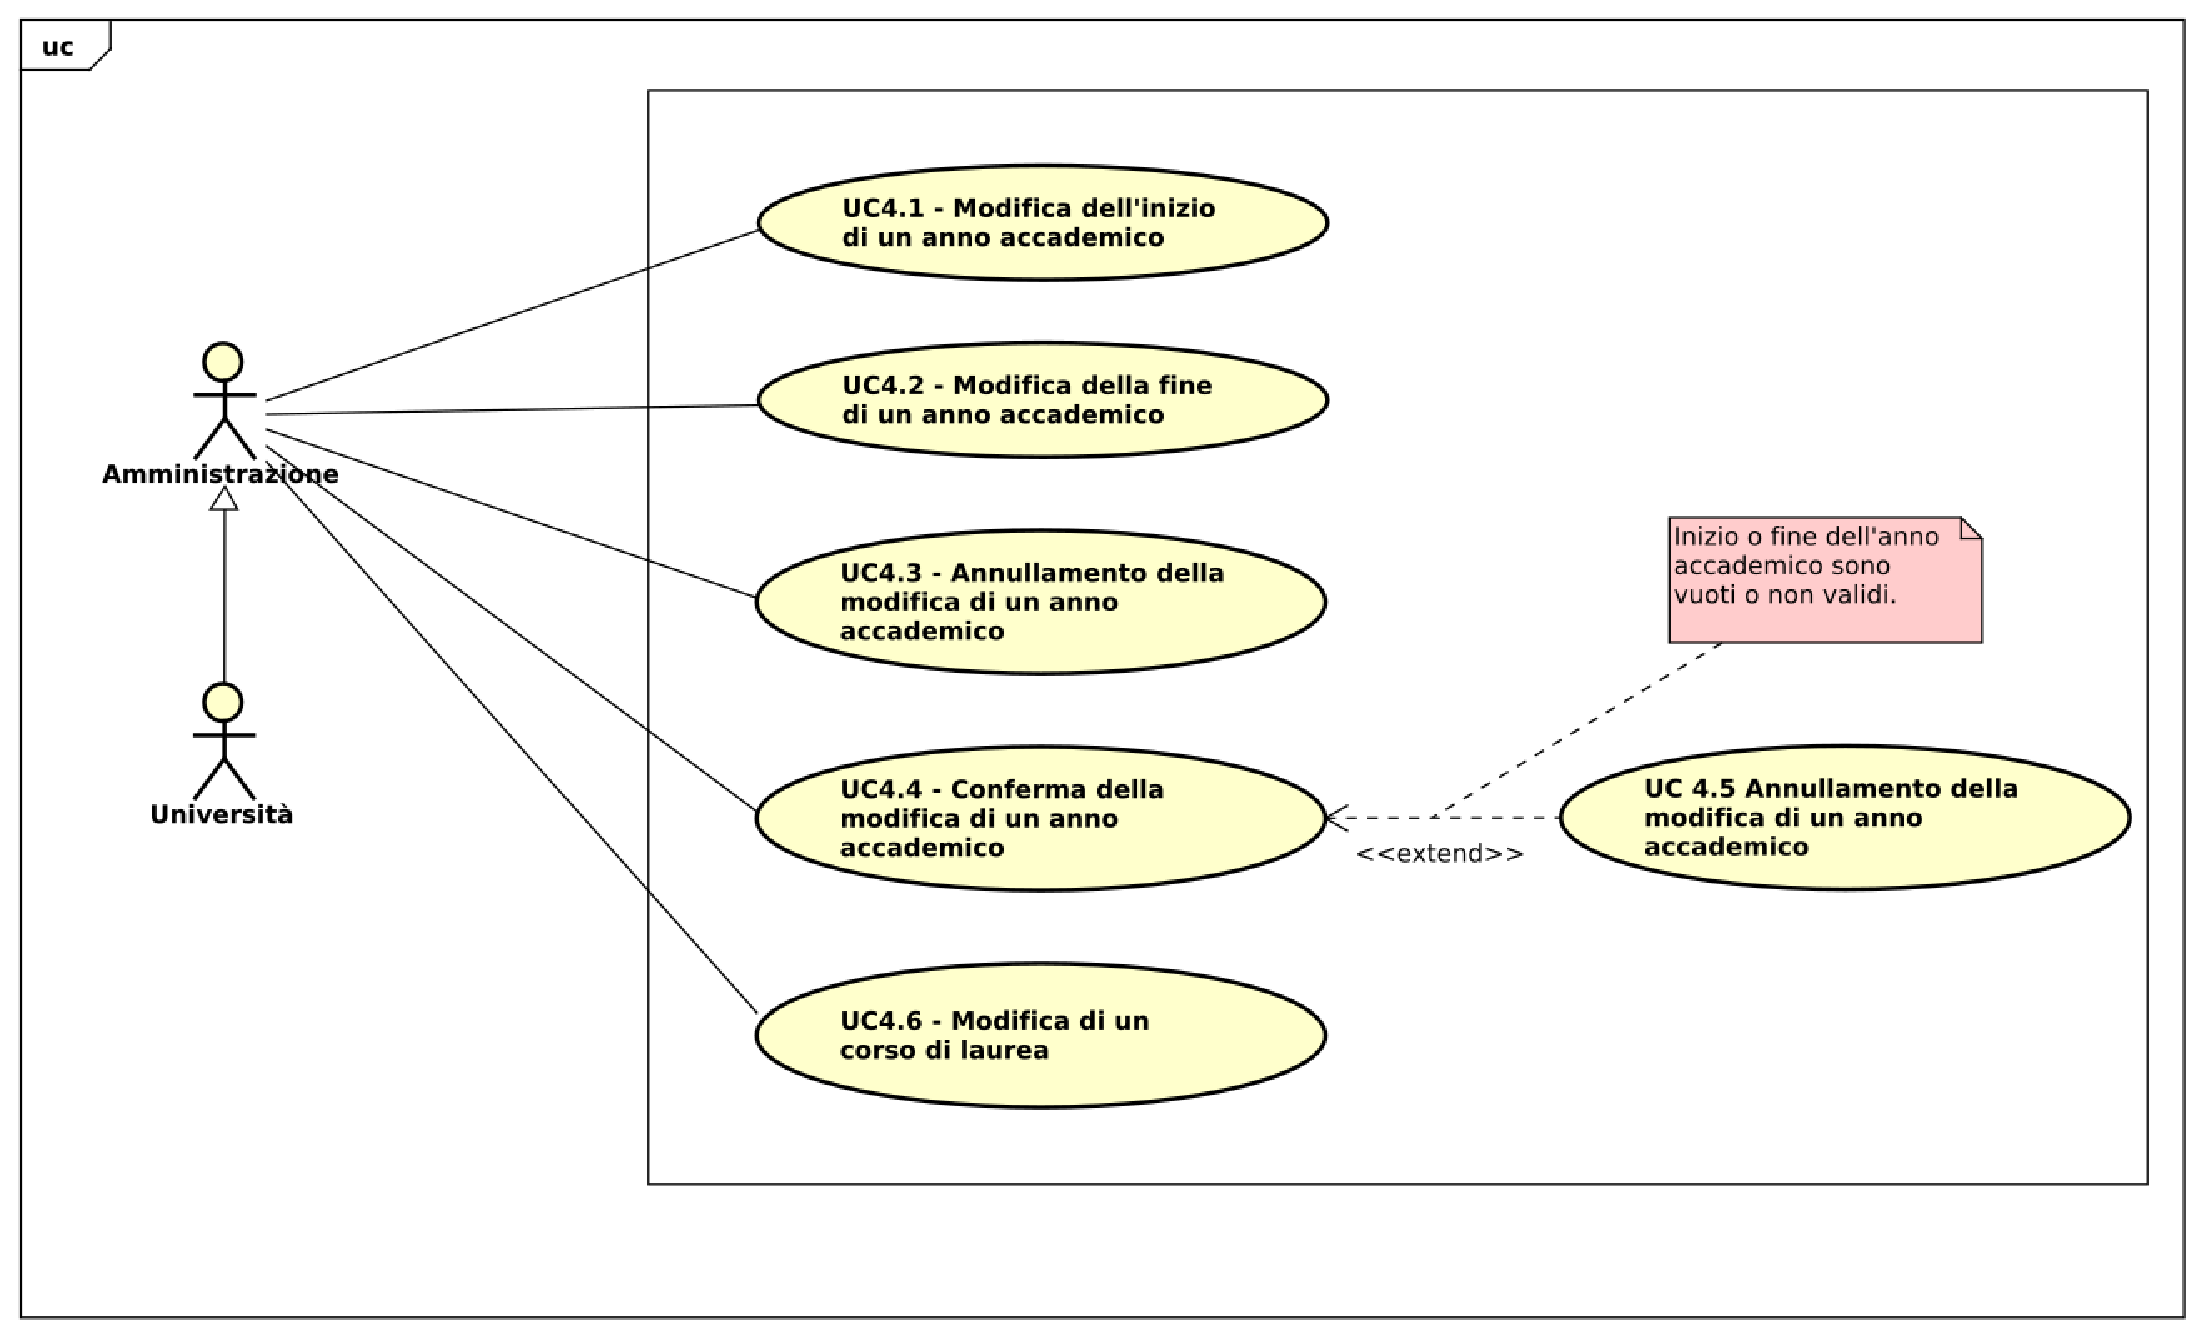
\includegraphics[scale=0.45]{./img/UC4.pdf}
	\caption{Modifica di un anno accademico}\label{}
\end{figure}
\begin{itemize}
	\item \textbf{Attori}: Amministratore, Università;
	\item \textbf{Descrizione}: L'attore può modificare un anno accademico dalla lista degli anni accademici;
	\item \textbf{Precondizione}: Il sistema fa visualizzare un anno accademico;
	\item \textbf{Flusso principale degli eventi}: L'attore per modificare un anno accademico deve seguire i seguenti punti:
	\begin{itemize}
		\item Modifica dell'inizio di un anno accademico (UC4.1);
		\item Modifica della fine di un anno accademico (UC4.2);
		\item Annullamento della modifica di un anno accademico (UC4.3);
		\item Conferma della modifica di un anno accademico (UC4.4);
		\item Visualizzazione dell'errore relativo alla modifica di un anno accademico (UC4.5);
		\item Modifica di un corso di laurea (UC4.6);
		\item Eliminazione di un corso di laurea (UC4.7);
		\item Visualizzazione dell'errore relativo all'eliminazione di un corso di laurea (UC4.8).
	\end{itemize}
	\item \textbf{Postcondizione}: Il sistema ha modificato l'anno accademico.
\end{itemize}
\subsection{Caso d'uso \texorpdfstring{UC4.1}{UC4.1}: Modifica dell'inizio di un anno accademico}
\begin{itemize}
	\item \textbf{Attori}: Amministratore, Università;
	\item \textbf{Descrizione}: L'attore modifica la data di partenza dell'anno accademico;
	\item \textbf{Precondizione}: Il sistema fa visualizzare un anno accademico;
	\item \textbf{Flusso principale degli eventi}: L'attore modifica la data di inizio dell'anno accademico precedentemente inserita;
	\item \textbf{Postcondizione}: Il sistema ha modificato l'inizio dell'anno accademico.
\end{itemize}
\subsection{Caso d'uso \texorpdfstring{UC4.2}{UC4.2}: Modifica della fine di un anno accademico}
\begin{itemize}
	\item \textbf{Attori}: Amministratore, Università;
	\item \textbf{Descrizione}: L'attore modifica la data di fine dell'anno accademico;
	\item \textbf{Precondizione}: Il sistema fa visualizzare un anno accademico;
	\item \textbf{Flusso principale degli eventi}: L'attore modifica la data di fine dell'anno accademico;
	\item \textbf{Postcondizione}: Il sistema ha modificato la data di fine dell'anno accademico.
\end{itemize}
\subsection{Caso d'uso \texorpdfstring{UC4.3}{UC4.3}: Annullamento della modifica di un anno accademico}
\begin{itemize}
	\item \textbf{Attori}: Amministratore, Università;
	\item \textbf{Descrizione}: L'attore annulla la modifica dell'anno accademico;
	\item \textbf{Precondizione}: Il sistema fa visualizzare la pagina relativa alla modifica di un anno accademico;
	\item \textbf{Flusso principale degli eventi}: L'attore una volta iniziata la modifica desidera annullare il processo;
	\item \textbf{Postcondizione}: Il sistema non modifica più un anno accademico in quanto l'attore ha annullato l'operazione.
\end{itemize}
\subsection{Caso d'uso \texorpdfstring{UC4.4}{UC4.4}: Conferma della modifica di un anno accademico}
\begin{itemize}
	\item \textbf{Attori}: Amministratore, Università;
	\item \textbf{Descrizione}: L'attore conferma la modifica relativa all'anno accademico;
	\item \textbf{Precondizione}: Il sistema fa visualizzare la pagina relativa alla modifica di un anno accademico;
	\item \textbf{Flusso principale degli eventi}: L'attore ha finito la modifica e desidera inserire nel sistema l'anno accademico modificato;
	\item \textbf{Postcondizione}: Il sistema modifica un anno accademico in quanto l'attore ha confermato l'operazione;
	\item \textbf{Estensioni}:
	\begin{itemize}
		\item Visualizzazione dell'errore relativo alla modifica di un anno accademico (UC4.5).
	\end{itemize}
\end{itemize}
\subsection{Caso d'uso \texorpdfstring{UC4.5}{UC4.5}: Visualizzazione dell'errore relativo alla modifica di un anno accademico}
\begin{itemize}
	\item \textbf{Attori}: Amministratore, Università;
	\item \textbf{Descrizione}: L'attore può visualizzare un errore nel caso avesse modificato erroneamente dei campi dati;
	\item \textbf{Precondizione}: Il sistema ha ricevuto campi dati errati o vuoti;
	\item \textbf{Flusso principale degli eventi}: L'attore, modificando in maniera errata i campi dell'anno accademico, può visualizzare uno dei seguenti errori: 
	\begin{itemize}
		\item Inizio dell'anno accademico non valido o lasciato vuoto; 
		\item Fine dell'anno accademico non valido o lasciato vuoto; 
		\item Nome dell'anno accademico non valido o lasciato vuoto. 
	\end{itemize}
	\item \textbf{Postcondizione}: Il sistema visualizza un messaggio d'errore relativo all'operazione di modifica di un anno accademico.
\end{itemize}
\subsection{Caso d'uso \texorpdfstring{UC4.6}{UC4.6}: Modifica di un corso di laurea}
\begin{figure} [H]
	\centering
	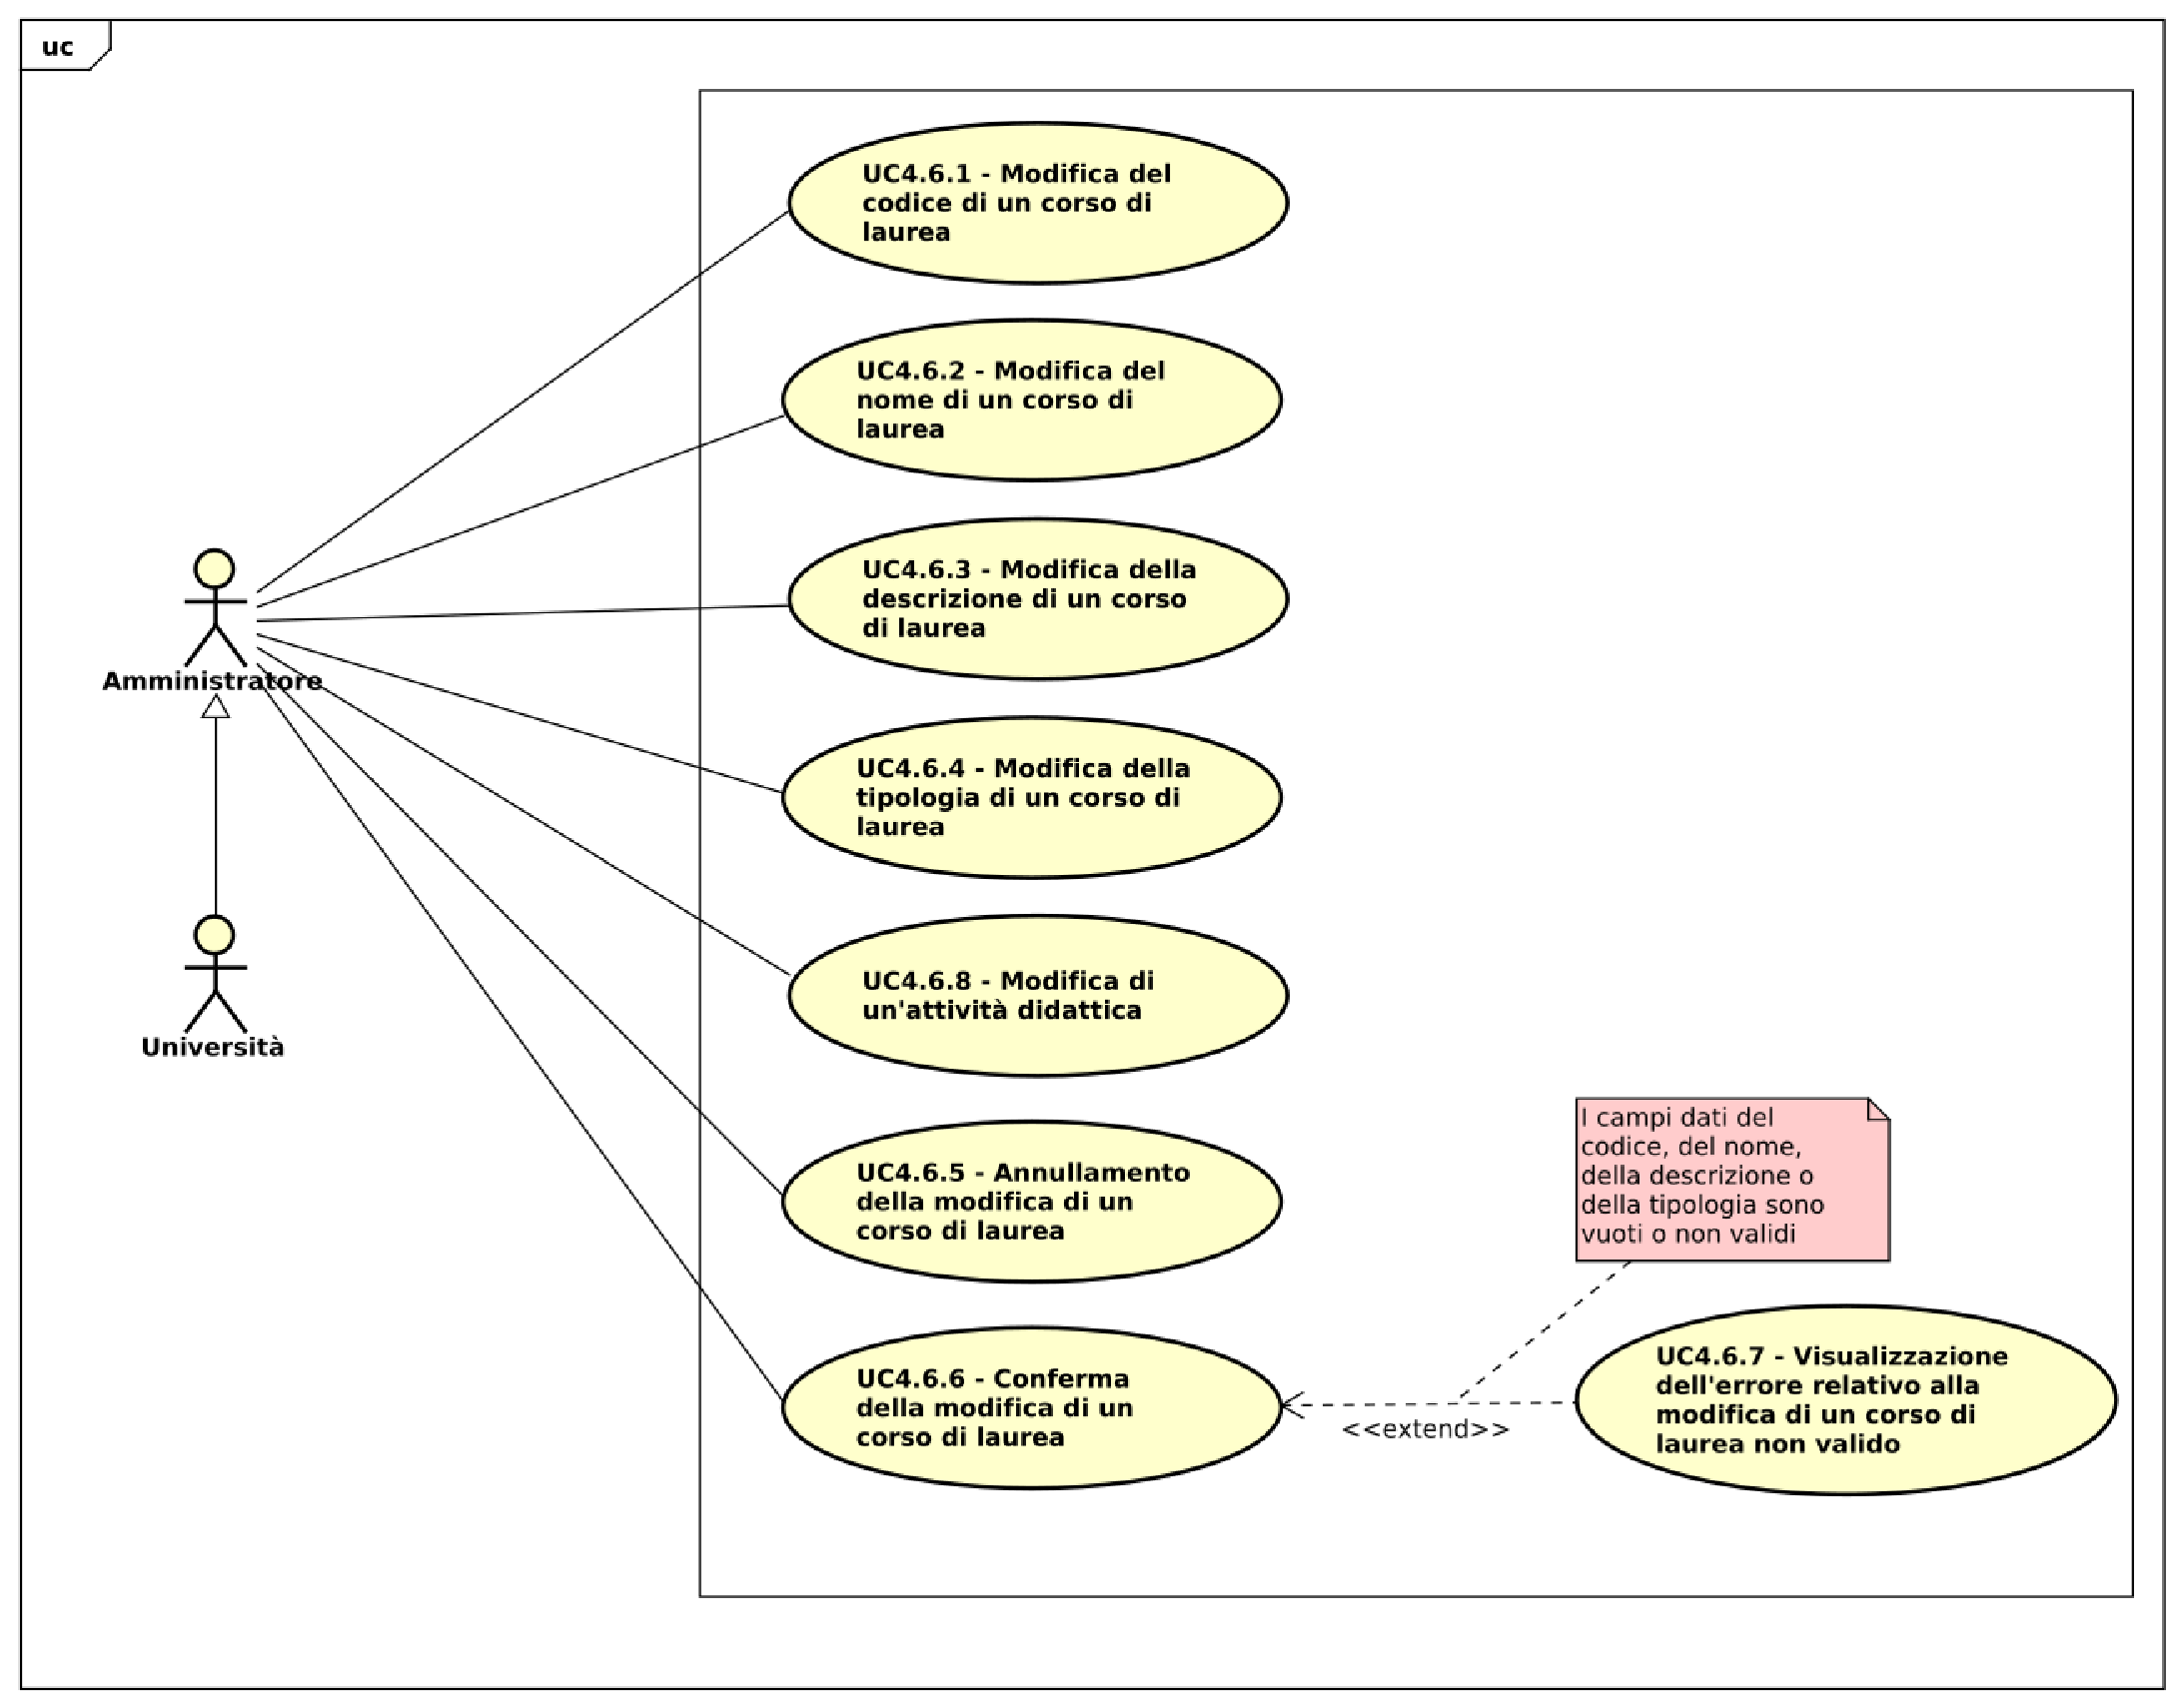
\includegraphics[scale=0.45]{./img/UC4-6.pdf}
	\caption{Modifica di un corso di laurea}\label{}
\end{figure}
\begin{itemize}
	\item \textbf{Attori}: Amministratore, Università;
	\item \textbf{Descrizione}: L'attore può modificare un corso di laurea dalla lista dei corsi di laurea;
	
	\item \textbf{Precondizione}: Il sistema fa visualizzare un corso di laurea;
	
	\item \textbf{Flusso principale degli eventi}: L'attore per modificare un corso di laurea deve seguire i seguenti punti:
	
	\begin{itemize}
		\item Modifica del codice di un corso di laurea (UC4.6.1);
		\item Modifica del nome di un corso di laurea (UC4.6.2);
		\item Modifica della descrizione di un corso di laurea (UC4.6.3);
		\item Modifica della tipologia di un corso di laurea (UC4.6.4);
		\item Annullamento della modifica di un corso di laurea (UC4.6.5);
		\item Conferma della modifica di un corso di laurea (UC4.6.6);
		\item Visualizzazione dell'errore relativo alla modifica di un corso di laurea non valido (UC4.6.7);
		\item Modifica di un'attività didattica (UC4.6.8);
		\item Eliminazione di un'attività didattica (UC4.6.9);
		\item Visualizzazione dell'errore relativo all'eliminazione di un'attività didattica (UC4.6.10).
	\end{itemize}
	\item \textbf{Postcondizione}: Il sistema ha modificato il corso di laurea.
	
\end{itemize}
\subsection{Caso d'uso \texorpdfstring{UC4.6.1}{UC4.6.1}: Modifica del codice di un corso di laurea}
\begin{itemize}
	\item \textbf{Attori}: Amministratore, Università;
	\item \textbf{Descrizione}: L'attore modifica il codice del corso di laurea;
	
	\item \textbf{Precondizione}: Il sistema fa visualizzare il campo di modifica del codice di un corso di laurea;
	\item \textbf{Flusso principale degli eventi}: L'attore modifica il codice del corso di laurea precedentemente inserito;
	
	\item \textbf{Postcondizione}: È stato modificato il codice del corso di laurea nel campo opportuno.
	
	
\end{itemize}
\subsection{Caso d'uso \texorpdfstring{UC4.6.2}{UC4.6.2}: Modifica del nome di un corso di laurea}
\begin{itemize}
	\item \textbf{Attori}: Amministratore, Università;
	\item \textbf{Descrizione}: L'attore modifica il nome del corso di laurea;
	
	\item \textbf{Precondizione}: Il sistema fa visualizzare il campo di modifica del nome di un corso di laurea;
	
	\item \textbf{Flusso principale degli eventi}: L'attore modifica il nome del corso di laurea precedentemente inserito;
	
	\item \textbf{Postcondizione}: È stato modificato il nome del corso di laurea nel campo opportuno.
	
	
\end{itemize}
\subsection{Caso d'uso \texorpdfstring{UC4.6.3}{UC4.6.3}: Modifica della descrizione di un corso di laurea}
\begin{itemize}
	\item \textbf{Attori}: Amministratore, Università;
	\item \textbf{Descrizione}: L'attore modifica la descrizione del corso di laurea;
	
	\item \textbf{Precondizione}: Il sistema fa visualizzare il campo di modifica della descrizione di un corso di laurea;
	
	\item \textbf{Flusso principale degli eventi}: L'attore modifica la descrizione del corso di laurea precedentemente inserita;
	
	\item \textbf{Postcondizione}: È stata modificata la descrizione del corso di laurea nel campo opportuno.
	
\end{itemize}
\subsection{Caso d'uso \texorpdfstring{UC4.6.4}{UC4.6.4}: Modifica della tipologia di un corso di laurea}
\begin{itemize}
	\item \textbf{Attori}: Amministratore, Università;
	\item \textbf{Descrizione}: L'attore modifica la tipologia del corso di laurea;
	
	\item \textbf{Precondizione}: Il sistema fa visualizzare il campo di modifica della tipologia di un corso di laurea;
	
	
	\item \textbf{Flusso principale degli eventi}: L'attore modifica la tipologia del corso di laurea precedentemente inserito;
	
	\item \textbf{Postcondizione}: È stata modificata la tipologia del corso di laurea nel campo opportuno.
	
\end{itemize}
\subsection{Caso d'uso \texorpdfstring{UC4.6.5}{UC4.6.5}: Annullamento della modifica di un corso di laurea}
\begin{itemize}
	\item \textbf{Attori}: Amministratore, Università;
	\item \textbf{Descrizione}: L'attore annulla la modifica del corso di laurea;
	
	\item \textbf{Precondizione}: l sistema fa visualizzare la pagina relativa alla modifica di un corso di laurea;
	
	\item \textbf{Flusso principale degli eventi}: L'attore una volta iniziata la modifica desidera annullare il processo;
	
	\item \textbf{Postcondizione}: Il sistema non modifica più un corso di laurea in quanto l'attore ha annullato l'operazione.
	
\end{itemize}
\subsection{Caso d'uso \texorpdfstring{UC4.6.6}{UC4.6.6}: Conferma della modifica di un corso di laurea}
\begin{itemize}
	\item \textbf{Attori}: Amministratore, Università;
	\item \textbf{Descrizione}: L'attore conferma la modifica relativa al corso di laurea;
	
	\item \textbf{Precondizione}: Il sistema fa visualizzare la pagina relativa alla modifica di un corso di laurea;
	
	
	\item \textbf{Flusso principale degli eventi}: L'attore ha finito la modifica e desidera inserire nel sistema il corso di laurea modificato;
	
	\item \textbf{Postcondizione}: Il sistema modifica un corso di laurea in quanto l'attore ha confermato l'operazione;
	
	\item \textbf{Estensioni}:
	\begin{itemize}
		\item Visualizzazione dell'errore relativo alla modifica di un corso di laurea non valido (UC4.6.7);
	\end{itemize}
\end{itemize}
\subsection{Caso d'uso \texorpdfstring{UC4.6.7}{UC4.6.7}: Visualizzazione dell'errore relativo alla modifica di un corso di laurea non valido}
\begin{itemize}
	\item \textbf{Attori}: Amministratore, Università;
	\item \textbf{Descrizione}: Il sistema visualizza un messaggio d'errore riguardante l'impossibilità di modificare un corso di laurea;
	
	\item \textbf{Precondizione}: Il sistema durante l'operazione di modifica ha ricevuto campi dati errati o vuoti;
	
	\item \textbf{Flusso principale degli eventi}: L'attore, modificando in maniera errata i campi del corso di laurea, può visualizzare uno dei seguenti errori: \begin{itemize} 
		\item Codice del corso di laurea non valido o lasciato vuoto; 
		\item Nome del corso di laurea non valido o lasciato vuoto; 
		\item Descrizione del corso di laurea non valido o lasciato vuoto; 
		\item Codice del corso di laurea non valido o lasciato vuoto; 
		\item Tipologia del corso di laurea non valido o lasciato vuoto; 
		\item Codice dell'anno accademico non valido o lasciato vuoto; 
		\item Attività didattica del corso di laurea non valida o lasciata vuota.
	\end{itemize}
	\item \textbf{Postcondizione}: Il sistema fa visualizzare un messaggio d'errore riguardante il tentativo di modificare un corso di laurea con campi dati errati o vuoti.
	
\end{itemize}
\subsection{Caso d'uso \texorpdfstring{UC4.6.8}{UC4.6.8}: Modifica di un'attività didattica}
\begin{figure} [H]
	\centering
	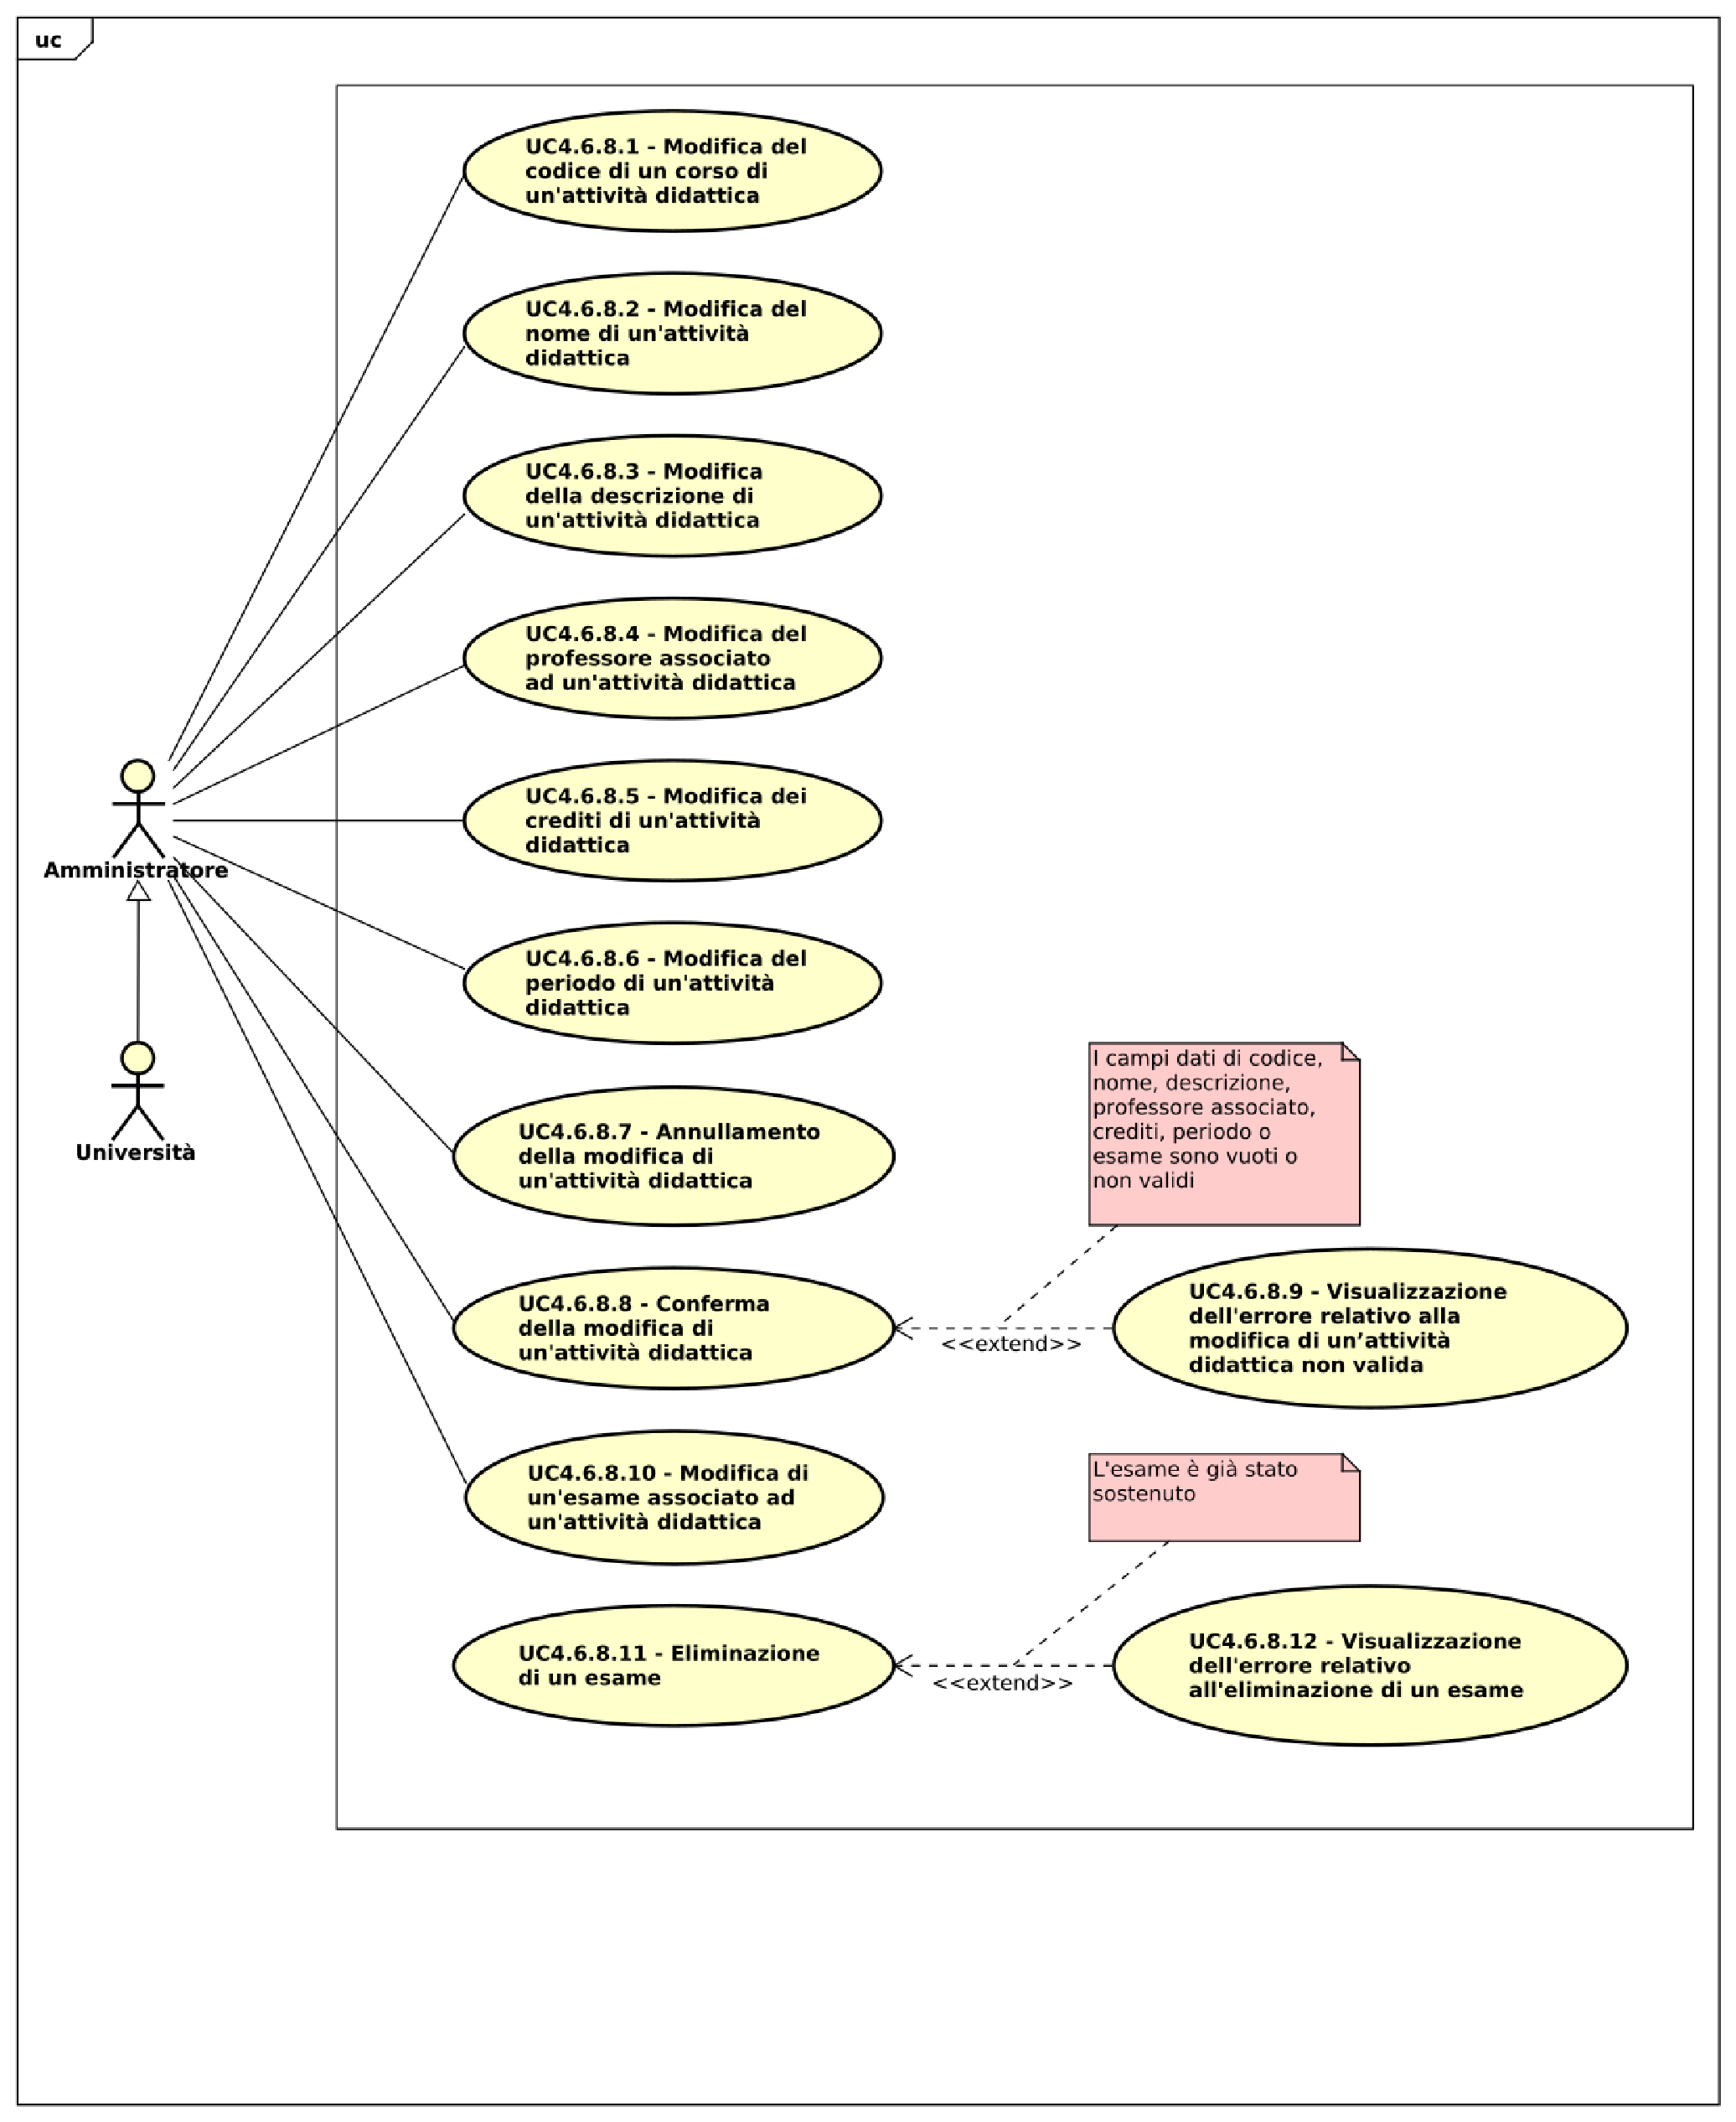
\includegraphics[scale=0.45]{./img/UC4-6-8.pdf}
	\caption{Modifica di un'attività didattica}\label{}
\end{figure}
\begin{itemize}
	\item \textbf{Attori}: Amministratore, Università;
	\item \textbf{Descrizione}: L'attore può modificare un’attività didattica dalla lista delle attività didattiche;
	
	\item \textbf{Precondizione}: Il sistema fa visualizzare un'attività didattica;
	
	\item \textbf{Flusso principale degli eventi}: L'attore per modificare un’attività didattica deve seguire i seguenti punti:
	
	\begin{itemize}
		\item Modifica del codice di un corso di un'attività didattica (UC4.6.8.1);
		\item Modifica del nome di un'attività didattica (UC4.6.8.2);
		\item Modifica della descrizione di un'attività didattica (UC4.6.8.3);
		\item Modifica del professore associato ad un'attività didattica (UC4.6.8.4);
		\item Modifica dei crediti di un'attività didattica (UC4.6.8.5);
		\item Modifica del periodo di un'attività didattica (UC4.6.8.6);
		\item Annullamento della modifica di un'attività didattica (UC4.6.8.7);
		\item Conferma della modifica di un'attività didattica (UC4.6.8.8);
		\item Visualizzazione dell'errore relativo alla modifica di un’attività didattica non valida (UC4.6.8.9);
		\item Modifica di un esame (UC4.6.8.10);
		\item Eliminazione di un esame (UC4.6.8.11);
		\item Visualizzazione dell'errore relativo all'eliminazione di un esame (UC4.6.8.12).
	\end{itemize}
	\item \textbf{Postcondizione}: Il sistema ha modificato un’attività didattica.
	
\end{itemize}
\subsection{Caso d'uso \texorpdfstring{UC4.6.8.1}{UC4.6.8.1}: Modifica del codice di un corso di un'attività didattica}
\begin{itemize}
	\item \textbf{Attori}: Amministratore, Università;
	\item \textbf{Descrizione}: L'attore modifica il codice del corso di un'attività didattica;
	
	\item \textbf{Precondizione}: Il sistema fa visualizzare un'attività didattica;
	
	\item \textbf{Flusso principale degli eventi}: L'attore modifica il codice del corso dell’attività didattica precedentemente inserito;
	
	\item \textbf{Postcondizione}: Il sistema ha modificato il codice del corso dell’attività didattica.
	
\end{itemize}
\subsection{Caso d'uso \texorpdfstring{UC4.6.8.2}{UC4.6.8.2}: Modifica del nome di un'attività didattica}
\begin{itemize}
	\item \textbf{Attori}: Amministratore, Università;
	\item \textbf{Descrizione}: L'attore modifica il nome di un'attività didattica;
	
	\item \textbf{Precondizione}: Il sistema fa visualizzare un'attività didattica;
	
	
	\item \textbf{Flusso principale degli eventi}: L'attore modifica il nome di un'attività didattica precedentemente inserito;
	
	\item \textbf{Postcondizione}: Il sistema ha modificato il nome di un'attività didattica.
	
\end{itemize}
\subsection{Caso d'uso \texorpdfstring{UC4.6.8.3}{UC4.6.8.3}: Modifica della descrizione di un'attività didattica}
\begin{itemize}
	\item \textbf{Attori}: Amministratore, Università;
	\item \textbf{Descrizione}: L'attore modifica la descrizione di un'attività didattica;
	
	\item \textbf{Precondizione}: Il sistema fa visualizzare un'attività didattica;
	
	
	\item \textbf{Flusso principale degli eventi}: L'attore modifica la descrizione di un'attività didattica precedentemente inserita;
	
	\item \textbf{Postcondizione}: Il sistema ha modificato la descrizione di un'attività didattica.
	
\end{itemize}
\subsection{Caso d'uso \texorpdfstring{UC4.6.8.4}{UC4.6.8.4}: Modifica del professore associato ad un'attività didattica}
\begin{itemize}
	\item \textbf{Attori}: Amministratore, Università;
	\item \textbf{Descrizione}: L'attore modifica il professore associato ad un'attività didattica;
	
	\item \textbf{Precondizione}: Il sistema fa visualizzare un'attività didattica;
	
	
	\item \textbf{Flusso principale degli eventi}: L'attore modifica il professore associato ad un'attività didattica precedentemente inserito;
	
	\item \textbf{Postcondizione}: Il sistema ha modificato il professore associato ad un'attività didattica.
	
\end{itemize}
\subsection{Caso d'uso \texorpdfstring{UC4.6.8.5}{UC4.6.8.5}: Modifica dei crediti di un'attività didattica}
\begin{itemize}
	\item \textbf{Attori}: Amministratore, Università;
	\item \textbf{Descrizione}: L'attore modifica i crediti di un'attività didattica;
	
	\item \textbf{Precondizione}: Il sistema fa visualizzare un'attività didattica;
	
	
	\item \textbf{Flusso principale degli eventi}: L'attore modifica i crediti di un'attività didattica precedentemente inseriti;
	
	\item \textbf{Postcondizione}: Il sistema ha modificato i crediti di un'attività didattica.
	
\end{itemize}
\subsection{Caso d'uso \texorpdfstring{UC4.6.8.6}{UC4.6.8.6}: Modifica del periodo di un'attività didattica}
\begin{itemize}
	\item \textbf{Attori}: Amministratore, Università;
	\item \textbf{Descrizione}: L'attore modifica il periodo di un'attività didattica;
	
	\item \textbf{Precondizione}: Il sistema fa visualizzare un'attività didattica;
	
	
	\item \textbf{Flusso principale degli eventi}: L'attore modifica il periodo di un'attività didattica precedentemente inserito;
	
	\item \textbf{Postcondizione}: Il sistema ha modificato il periodo di un'attività didattica.
	
\end{itemize}
\subsection{Caso d'uso \texorpdfstring{UC4.6.8.7}{UC4.6.8.7}: Annullamento della modifica di un'attività didattica}
\begin{itemize}
	\item \textbf{Attori}: Amministratore, Università;
	\item \textbf{Descrizione}: L'attore annulla la di un'attività didattica;
	
	\item \textbf{Precondizione}: Il sistema fa visualizzare la pagina relativa alla modifica di un'attività didattica;
	
	\item \textbf{Flusso principale degli eventi}: L'attore una volta iniziata la modifica desidera annullare il processo;
	
	\item \textbf{Postcondizione}: Il sistema non modifica più un'attività didattica in quanto l'attore ha annullato l'operazione.
	
\end{itemize}
\subsection{Caso d'uso \texorpdfstring{UC4.6.8.8}{UC4.6.8.8}: Conferma della modifica di un'attività didattica}
\begin{itemize}
	\item \textbf{Attori}: Amministratore, Università;
	\item \textbf{Descrizione}: L'attore conferma la modifica relativa ad un'attività didattica;
	
	\item \textbf{Precondizione}: Il sistema fa visualizzare la pagina relativa alla modifica di un'attività didattica;
	
	
	\item \textbf{Flusso principale degli eventi}: L'attore ha finito la modifica e desidera inserire nel sistema l'attività didattica modificata;
	
	\item \textbf{Postcondizione}: Il sistema modifica un'attività didattica in quanto l'attore ha confermato l'operazione;
	
	
	\item \textbf{Estensioni}:
	\begin{itemize}
		\item Visualizzazione dell'errore relativo alla modifica di un’attività didattica non valida (UC4.6.8.9).
	\end{itemize}
\end{itemize}
\subsection{Caso d'uso \texorpdfstring{UC4.6.8.9}{UC4.6.8.9}: Visualizzazione dell'errore relativo alla modifica di un’attività didattica non valida}
\begin{itemize}
	\item \textbf{Attori}: Amministratore, Università;
	\item \textbf{Descrizione}: Il sistema visualizza un messaggio d'errore riguardante l'impossibilità di modificare di un'attività didattica;
	
	\item \textbf{Precondizione}: Il sistema ha ricevuto campi dati errati o vuoti;
	
	\item \textbf{Flusso principale degli eventi}: L'attore, modificando in maniera errata i campi di un'attività didattica, può visualizzare uno dei seguenti errori: 
	\begin{itemize} 
		\item Codice del corso dell’attività didattica non valido o lasciato vuoto; 
		\item Nome dell’attività didattica non valido o lasciato vuoto;
		\item Descrizione dell’attività didattica non valida o lasciato vuoto; 
		\item Professore associato all’attività didattica non valido o lasciato vuoto;
		\item Crediti dell’attività didattica non validi o lasciato vuoto; 
		\item Periodo dell’attività didattica non valido o lasciato vuoto; 
		\item Esame associato all’attività didattica non valido o lasciato vuoto. 
	\end{itemize}
	\item \textbf{Postcondizione}: Il sistema visualizza un messaggio d'errore relativo all'operazione di modifica di un'attività didattica.
	
	
\end{itemize}
\subsection{Caso d'uso \texorpdfstring{UC4.6.8.10}{UC4.6.8.10}: Modifica di un esame}
\begin{figure} [H]
	\centering
	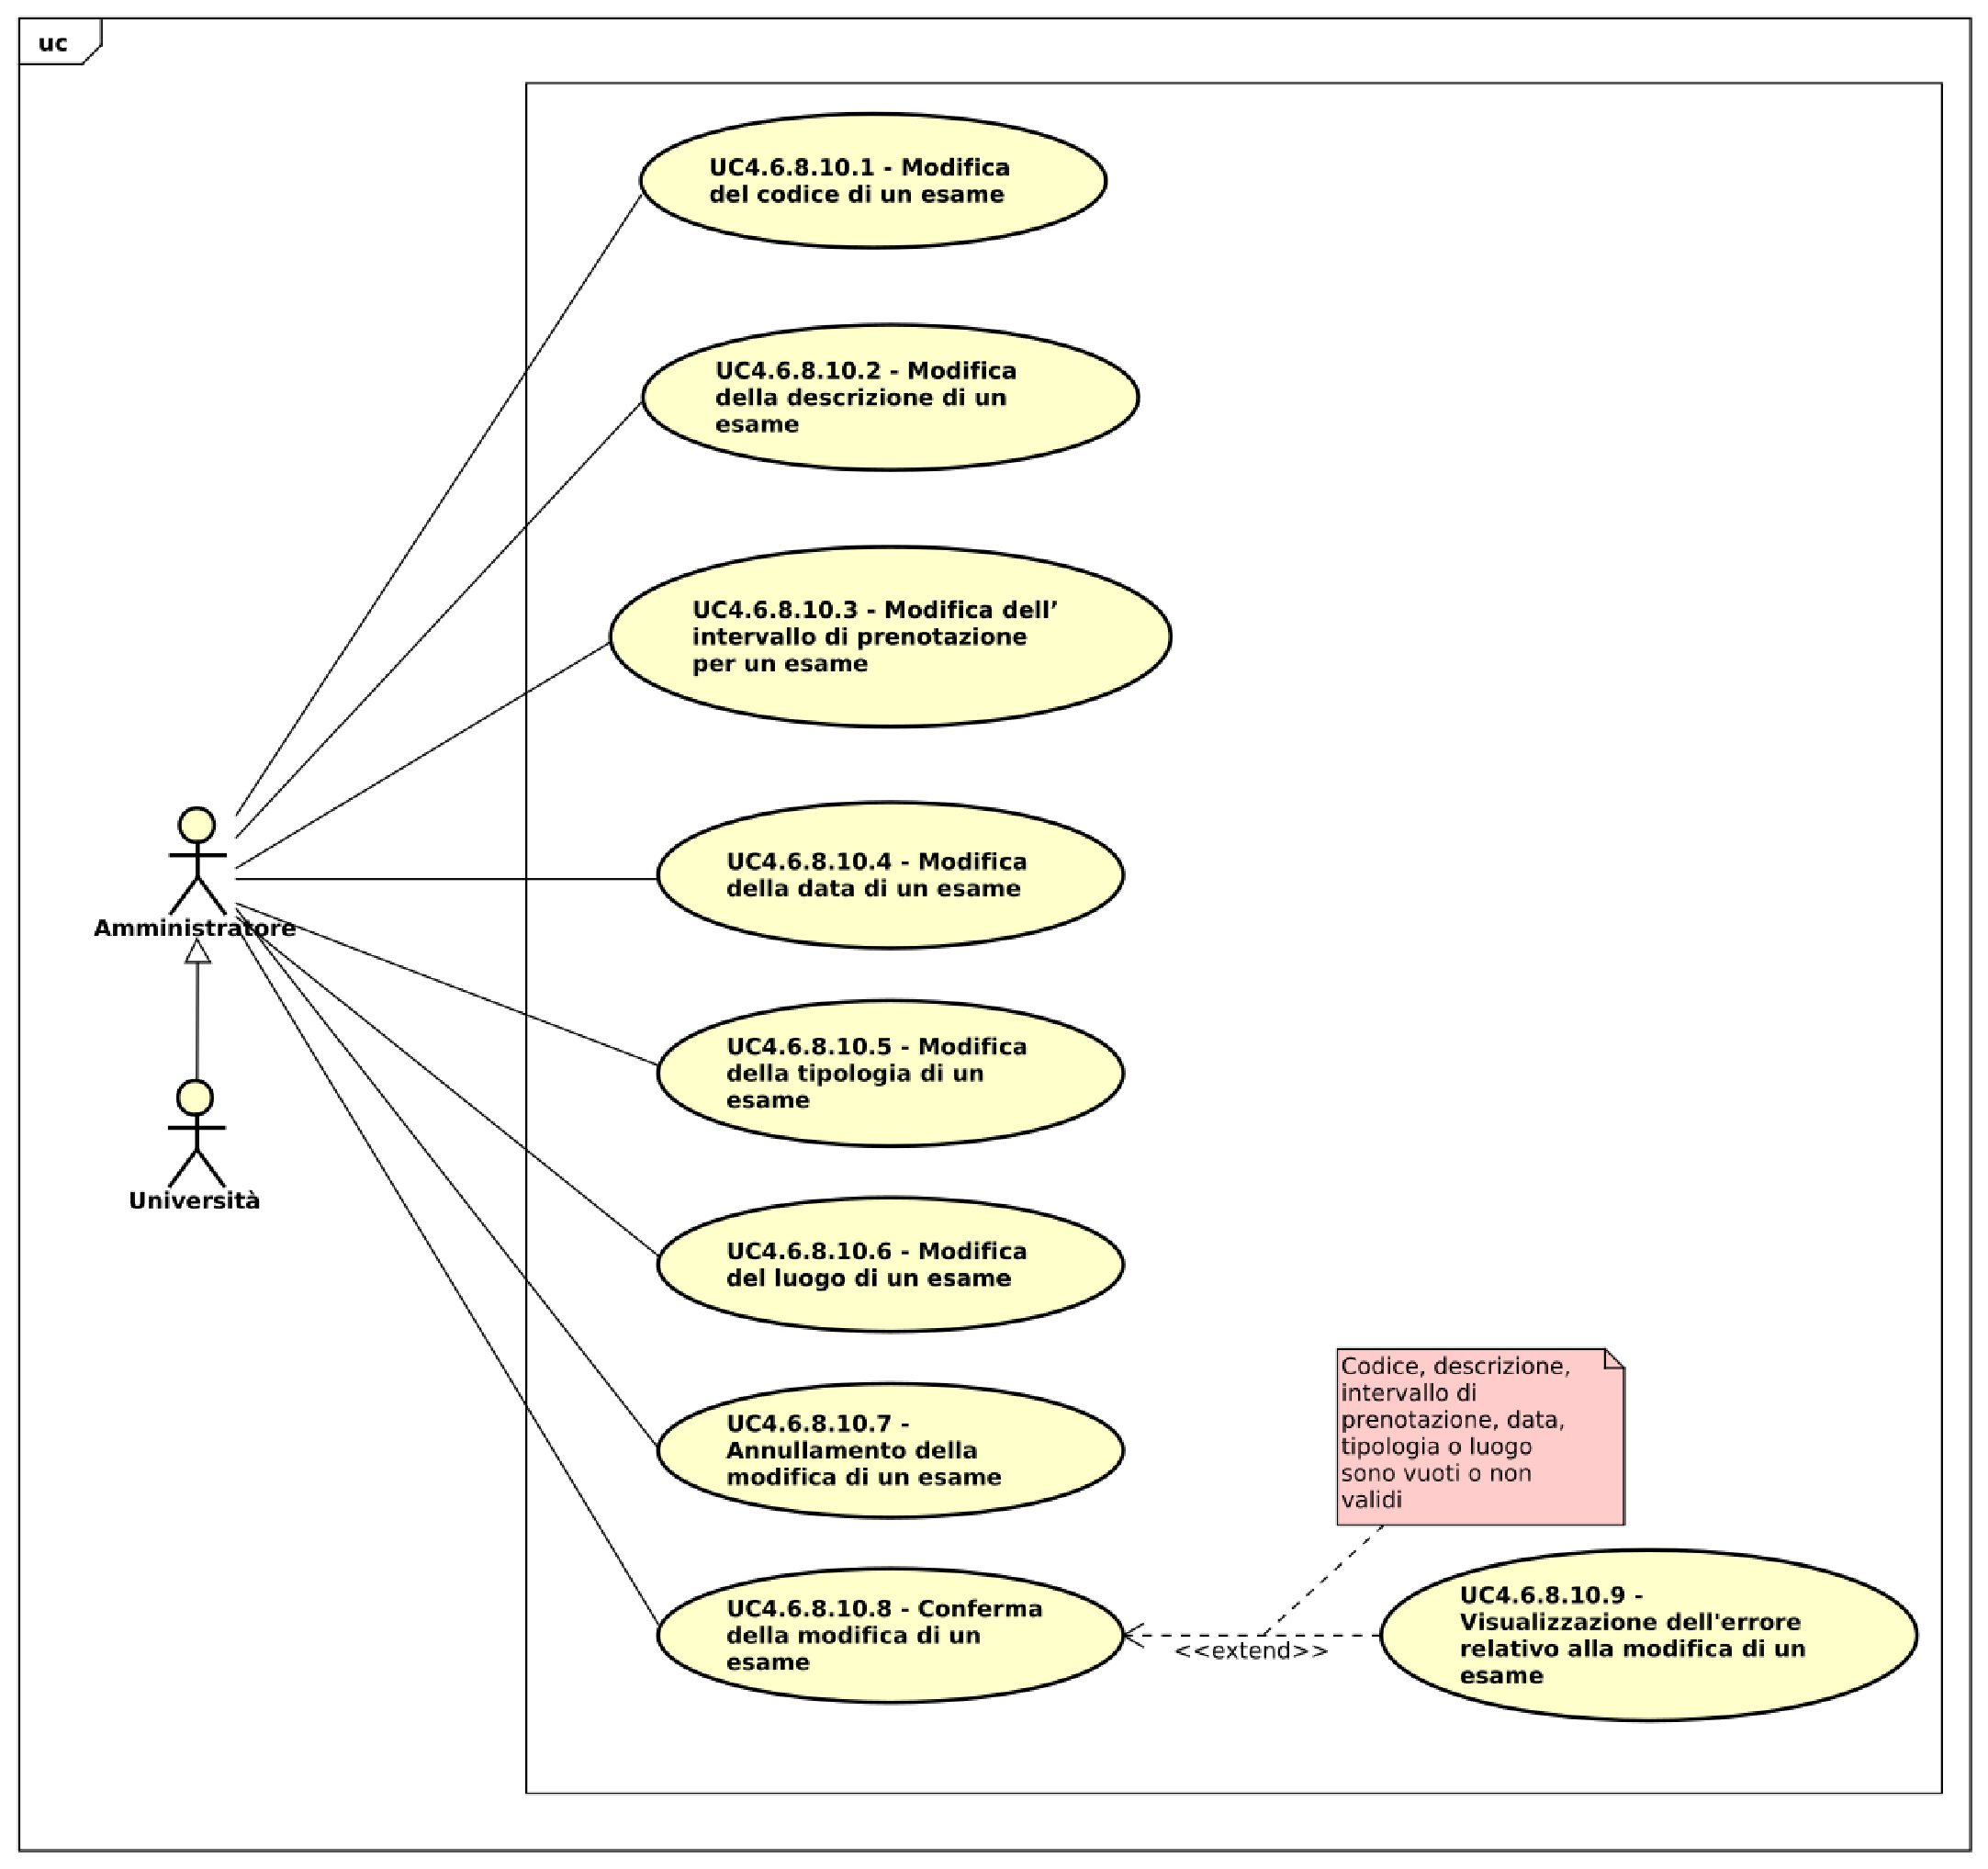
\includegraphics[scale=0.45]{./img/UC4-6-8-10.pdf}
	\caption{Modifica di un esame}\label{}
\end{figure}
\begin{itemize}
	\item \textbf{Attori}: Amministratore, Università;
	\item \textbf{Descrizione}: L'attore può modificare un esame dalla lista degli esami;
	
	\item \textbf{Precondizione}: Il sistema fa visualizzare un esame;
	
	\item \textbf{Flusso principale degli eventi}: L'attore per modificare un esame deve seguire i seguenti punti:
	
	\begin{itemize}
		\item Modifica del codice di un esame (UC4.6.8.10.1);
		\item Modifica della descrizione di un esame (UC4.6.8.10.2);
		\item Modifica dell’intervallo di prenotazione di un esame (UC4.6.8.10.3);
		\item Modifica della data di un esame (UC4.6.8.10.4);
		\item Modifica della tipologia di un esame (UC4.6.8.10.5);
		\item Modifica del luogo di un esame (UC4.6.8.10.6);
		\item Annullamento della modifica di un esame (UC4.6.8.10.7);
		\item Conferma della modifica di un esame (UC4.6.8.10.8);
		\item Visualizzazione dell'errore relativo alla modifica di un esame (UC4.6.8.10.9).
	\end{itemize}
	\item \textbf{Postcondizione}: Il sistema ha modificato l'esame.
	
\end{itemize}
\subsection{Caso d'uso \texorpdfstring{UC4.6.8.10.1}{UC4.6.8.10.1}: Modifica del codice di un esame}
\begin{itemize}
	\item \textbf{Attori}: Amministratore, Università;
	\item \textbf{Descrizione}: L'attore modifica il codice di un esame;
	
	\item \textbf{Precondizione}: Il sistema fa visualizzare un esame;
	
	
	\item \textbf{Flusso principale degli eventi}: L'attore modifica il codice di un esame precedentemente inserito;
	
	\item \textbf{Postcondizione}: Il sistema ha modificato il codice dell’esame.
	
\end{itemize}
\subsection{Caso d'uso \texorpdfstring{UC4.6.8.10.2}{UC4.6.8.10.2}: Modifica della descrizione di un esame}
\begin{itemize}
	\item \textbf{Attori}: Amministratore, Università;
	\item \textbf{Descrizione}: L'attore modifica la descrizione di un esame;
	
	\item \textbf{Precondizione}: Il sistema fa visualizzare un esame;
	
	\item \textbf{Flusso principale degli eventi}: L'attore modifica la descrizione dell’esame precedentemente inserita;
	
	\item \textbf{Postcondizione}: Il sistema ha modificato la descrizione dell’esame.
	
\end{itemize}
\subsection{Caso d'uso \texorpdfstring{UC4.6.8.10.3}{UC4.6.8.10.3}: Modifica dell’intervallo di prenotazione di un esame}
\begin{itemize}
	\item \textbf{Attori}: Amministratore, Università;
	\item \textbf{Descrizione}: L'attore modifica l'intervallo di prenotazione di un esame;
	
	\item \textbf{Precondizione}: Il sistema fa visualizzare un esame;
	
	\item \textbf{Flusso principale degli eventi}: L'attore modifica l'intervallo di prenotazione per l’esame;
	
	\item \textbf{Postcondizione}: Il sistema ha modificato l'intervallo di prenotazione per l’esame.
	
\end{itemize}
\subsection{Caso d'uso \texorpdfstring{UC4.6.8.10.4}{UC4.6.8.10.4}: Modifica della data di un esame}
\begin{itemize}
	\item \textbf{Attori}: Amministratore, Università;
	\item \textbf{Descrizione}: L'attore modifica la data di un esame;
	
	\item \textbf{Precondizione}: Il sistema fa visualizzare un esame;
	
	\item \textbf{Flusso principale degli eventi}: L'attore modifica la data di un esame precedentemente inserito;
	
	\item \textbf{Postcondizione}: Il sistema ha modificato la data dell'esame.
	
\end{itemize}
\subsection{Caso d'uso \texorpdfstring{UC4.6.8.10.5}{UC4.6.8.10.5}: Modifica della tipologia di un esame}
\begin{itemize}
	\item \textbf{Attori}: Amministratore, Università;
	\item \textbf{Descrizione}: L'attore modifica la tipologia di un esame;
	
	\item \textbf{Precondizione}: Il sistema fa visualizzare un esame;
	
	\item \textbf{Flusso principale degli eventi}: L'attore modifica la tipologia di un esame precedentemente inserito;
	
	\item \textbf{Postcondizione}: Il sistema ha modificato la tipologia dell’esame.
	
\end{itemize}
\subsection{Caso d'uso \texorpdfstring{UC4.6.8.10.6}{UC4.6.8.10.6}: Modifica del luogo di un esame}
\begin{itemize}
	\item \textbf{Attori}: Amministratore, Università;
	\item \textbf{Descrizione}: L'attore modifica il luogo di un esame;
	
	\item \textbf{Precondizione}: Il sistema fa visualizzare un esame;
	
	\item \textbf{Flusso principale degli eventi}: L'attore modifica il luogo di un esame precedentemente inserito;
	
	\item \textbf{Postcondizione}: Il sistema ha modificato il luogo dell'esame.
	
\end{itemize}
\subsection{Caso d'uso \texorpdfstring{UC4.6.8.10.7}{UC4.6.8.10.7}: Annullamento della modifica di un esame}
\begin{itemize}
	\item \textbf{Attori}: Amministratore, Università;
	\item \textbf{Descrizione}: L'attore annulla la modifica di un esame;
	
	\item \textbf{Precondizione}: Il sistema fa visualizzare la pagina relativa alla modifica di un esame;
	
	
	\item \textbf{Flusso principale degli eventi}: L'attore una volta iniziata la modifica desidera annullare il processo;
	
	\item \textbf{Postcondizione}: Il sistema non modifica più un esame in quanto l'attore ha annullato l'operazione.
	
	
\end{itemize}
\subsection{Caso d'uso \texorpdfstring{UC4.6.8.10.8}{UC4.6.8.10.8}: Conferma della modifica di un esame}
\begin{itemize}
	\item \textbf{Attori}: Amministratore, Università;
	\item \textbf{Descrizione}: L'attore conferma la modifica relativa ad un esame;
	
	\item \textbf{Precondizione}: Il sistema fa visualizzare la pagina relativa alla modifica di un esame;
	
	\item \textbf{Flusso principale degli eventi}: L'attore ha finito la modifica e desidera inserire nel sistema l'esame modificato;
	
	\item \textbf{Postcondizione}: Il sistema modifica un esame in quanto l'attore ha confermato l'operazione;
	
	
	\item \textbf{Estensioni}:
	\begin{itemize}
		\item Visualizzazione dell'errore relativo alla modifica di un esame (UC4.6.8.10.9).
	\end{itemize}
\end{itemize}
\subsection{Caso d'uso \texorpdfstring{UC4.6.8.10.9}{UC4.6.8.10.9}: Visualizzazione dell'errore relativo alla modifica di un esame}
\begin{itemize}
	\item \textbf{Attori}: Amministratore, Università;
	\item \textbf{Descrizione}: Il sistema visualizza un messaggio d'errore riguardante l'impossibilità di modificare un esame;
	
	\item \textbf{Precondizione}: Il sistema ha ricevuto campi dati errati o vuoti;
	
	
	\item \textbf{Flusso principale degli eventi}: L'attore, modificando in maniera errata i campi dell'esame, può visualizzare uno dei seguenti errori: \begin{itemize} 
		\item Codice dell’esame non valido o lasciato vuoto; 
		\item Descrizione dell’esame non valida o lasciato vuoto; 
		\item Intervallo di prenotazione per l’esame non valido o lasciato vuoto; 
		\item Data dell’esame non valida o lasciato vuoto; 
		\item Tipologia dell’esame non valida o lasciato vuoto; 
		\item Luogo d’esame non valido o lasciato vuoto.
	\end{itemize}
	\item \textbf{Postcondizione}: Il sistema visualizza un messaggio d'errore relativo all'operazione di modifica di un esame
	
	
\end{itemize}
\subsection{Caso d'uso \texorpdfstring{UC4.6.8.11}{UC4.6.8.11}: Eliminazione di un esame}
\begin{itemize}
	\item \textbf{Attori}: Amministratore, Università;
	\item \textbf{Descrizione}: L'attore elimina un esame;
	
	\item \textbf{Precondizione}: Il sistema fa visualizzare la lista degli esami;
	
	\item \textbf{Flusso principale degli eventi}: L'attore desidera eliminare un esame;
	
	\item \textbf{Postcondizione}: Il sistema ha eliminato un esame dalla lista degli esami.
	
	\item \textbf{Estensioni}:
	\begin{itemize}
		\item Visualizzazione dell'errore relativo all'eliminazione di un esame (UC4.6.8.12).
	\end{itemize}
\end{itemize}
\subsection{Caso d'uso \texorpdfstring{UC4.6.8.12}{UC4.6.8.12}: Visualizzazione dell'errore relativo all'eliminazione di un esame}
\begin{itemize}
	\item \textbf{Attori}: Amministratore, Università;
	\item \textbf{Descrizione}: Il sistema visualizza un messaggio d'errore riguardante l'impossibilità di eliminazione di un esame;
	\item \textbf{Precondizione}: Il sistema fa visualizzare uno specifico esame;
	
	\item \textbf{Flusso principale degli eventi}: L'attore cercando di eliminare l'esame visualizza un messaggio d'errore;
	\item \textbf{Postcondizione}: Il sistema fa visualizzare un messaggio d'errore riguardante l'impossibilità di eliminazione di un esame.
\end{itemize}
\subsection{Caso d'uso \texorpdfstring{UC4.6.9}{UC4.6.9}: Eliminazione di un'attività didattica}
\begin{itemize}
	\item \textbf{Attori}: Amministratore, Università;
	\item \textbf{Descrizione}: L'attore elimina un'attività didattica;
	
	\item \textbf{Precondizione}: Il sistema fa visualizzare la lista delle attività didattiche;
	
	\item \textbf{Flusso principale degli eventi}: L'attore desidera eliminare un'attività didattica;
	
	\item \textbf{Postcondizione}: Il sistema ha eliminato un'attività didattica dalla lista delle attività didattiche;
	
	\item \textbf{Estensioni}:
	\begin{itemize}
		\item Visualizzazione dell'errore relativo all'eliminazione di un'attività didattica (UC4.6.10).
	\end{itemize}
\end{itemize}
\subsection{Caso d'uso \texorpdfstring{UC4.6.10}{UC4.6.10}: Visualizzazione dell'errore relativo all'eliminazione di un'attività didattica}
\begin{itemize}
	\item \textbf{Attori}: Amministratore, Università;
	\item \textbf{Descrizione}: Il sistema visualizza un messaggio d'errore riguardante l'impossibilità di eliminazione di un'attività didattica;
	
	\item \textbf{Precondizione}: Il sistema fa visualizzare una specifica attività didattica;
	
	\item \textbf{Flusso principale degli eventi}: L'attore cercando di eliminare l'attività didattica in corso visualizza un messaggio d'errore;
	
	\item \textbf{Postcondizione}: Il sistema fa visualizzare un messaggio d'errore riguardante l'impossibilità di eliminazione di un'attività didattica.
	
\end{itemize}
\subsection{Caso d'uso \texorpdfstring{UC4.7}{UC4.7}: Eliminazione di un corso di laurea}
\begin{itemize}
	\item \textbf{Attori}: Amministratore, Università;
	\item \textbf{Descrizione}: L'attore elimina un corso di laurea;
	
	\item \textbf{Precondizione}: Il sistema fa visualizzare la lista dei corsi di laurea;
	
	
	\item \textbf{Flusso principale degli eventi}: L'attore desidera eliminare un corso di laurea;
	
	\item \textbf{Postcondizione}: Il sistema ha eliminato un corso di laurea dalla lista dei corsi di laurea.
	
	
	\item \textbf{Estensioni}:
	\begin{itemize}
		\item Visualizzazione dell'errore relativo all'eliminazione di un corso di laurea (UC4.8).
	\end{itemize}
\end{itemize}
\subsection{Caso d'uso \texorpdfstring{UC4.8}{UC4.8}: Visualizzazione dell'errore relativo all'eliminazione di un corso di laurea}
\begin{itemize}
	\item \textbf{Attori}: Amministratore, Università;
	\item \textbf{Descrizione}: Il sistema visualizza un messaggio d'errore riguardante l'impossibilità di eliminazione di un corso di laurea;
	
	\item \textbf{Precondizione}: Il sistema fa visualizzare uno specifico corso di laurea;
	
	
	\item \textbf{Flusso principale degli eventi}: L'attore cercando di eliminare il corso di laurea in corso visualizza un messaggio d'errore;
	
	\item \textbf{Postcondizione}: Il sistema fa visualizzare un messaggio d'errore riguardante l'impossibilità di eliminazione di un corso di laurea.
	
\end{itemize}
\subsection{Caso d'uso \texorpdfstring{UC5}{UC5}: Eliminazione di un anno accademico}
\begin{itemize}
	\item \textbf{Attori}: Amministratore, Università;
	\item \textbf{Descrizione}: L'attore elimina un anno accademico;
	\item \textbf{Precondizione}: Il sistema fa visualizzare la lista degli anni accademici;
	\item \textbf{Flusso principale degli eventi}: L'attore desidera eliminare un anno accademico;
	\item \textbf{Postcondizione}: Il sistema ha eliminato un anno accademico dalla lista degli anni accademici.
	
	\item \textbf{Estensioni}:
	\begin{itemize}
		\item Visualizzazione dell'errore relativo all'eliminazione di un anno accademico (UC13).
	\end{itemize}
\end{itemize}
\subsection{Caso d'uso \texorpdfstring{UC6}{UC6}: Iscrizione ad un esame}
\begin{figure} [H]
	\centering
	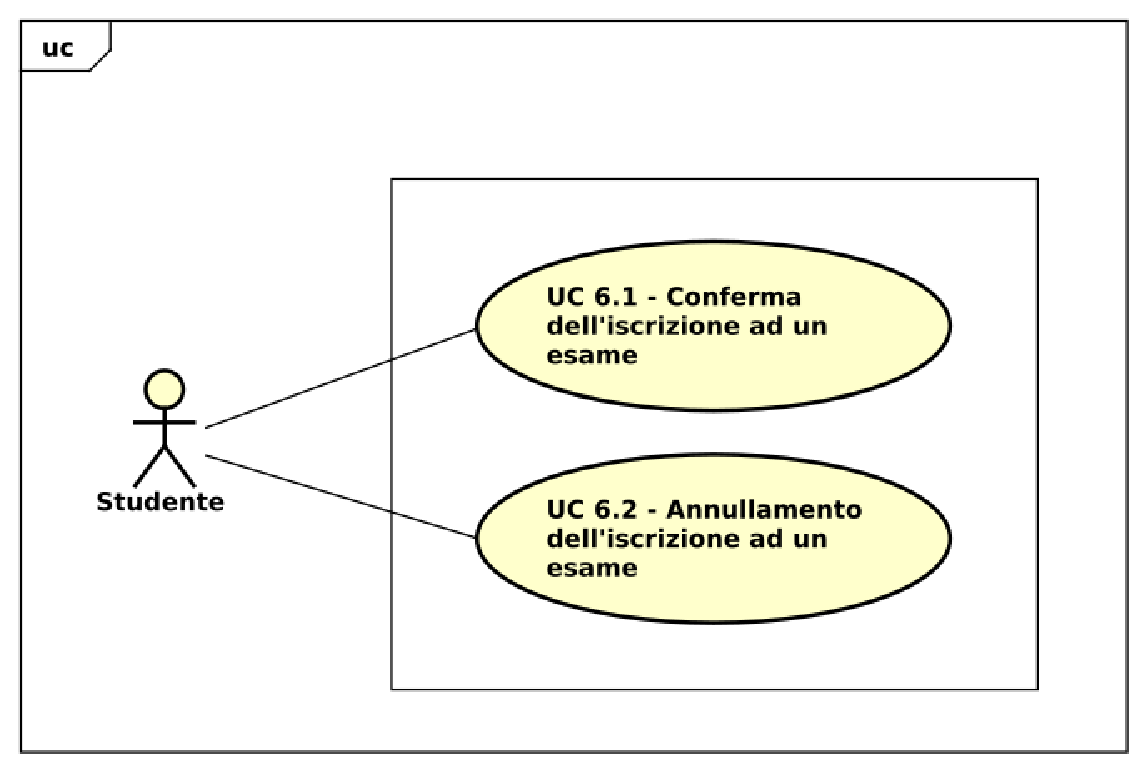
\includegraphics[scale=0.45]{./img/UC6.pdf}
	\caption{Iscrizione ad un esame}\label{}
\end{figure}
\begin{itemize}
	\item \textbf{Attori}: Studente;
	\item \textbf{Descrizione}: L'attore vedendo la lista degli appelli disponibili si iscrive ad uno di essi;
	\item \textbf{Precondizione}: Il sistema fa visualizzare la lista degli appelli disponibili per l'attore;
	\item \textbf{Flusso principale degli eventi}: L'attore si iscrive ad un esame;
	\begin{itemize}
		\item Conferma dell'iscrizione ad un esame (UC6.1);
		\item Annullamento dell'iscrizione ad un esame (UC6.2).
	\end{itemize}
	\item \textbf{Postcondizione}: Il sistema fa visualizzare l'appello che l'attore ha selezionato per l'iscrizione.
\end{itemize}
\subsection{Caso d'uso \texorpdfstring{UC6.1}{UC6.1}: Conferma dell'iscrizione ad un esame}
\begin{itemize}
	\item \textbf{Attori}: Studente;
	\item \textbf{Descrizione}: L'attore può confermare l'azione di iscrizione ad un esame;
	\item \textbf{Precondizione}: Il sistema fa visualizzare all'attore l'esame che ha selezionato per l'iscrizione;
	\item \textbf{Flusso principale degli eventi}: L'attore ha selezionato l'esame a cui iscriversi e può confermare l'azione;
	\item \textbf{Postcondizione}: Il sistema ha iscritto l'attore a quell'esame.
\end{itemize}
\subsection{Caso d'uso \texorpdfstring{UC6.2}{UC6.2}: Annullamento dell'iscrizione ad un esame}
\begin{itemize}
	\item \textbf{Attori}: Studente;
	\item \textbf{Descrizione}: L'attore può annullare l'azione di iscrizione ad un esame;
	\item \textbf{Precondizione}: Il sistema fa visualizzare all'attore l'esame che ha selezionato per l'iscrizione;
	
	\item \textbf{Flusso principale degli eventi}: L'attore può annullare l'iscrizione ad un esame dopo averlo selezionato;
	\item \textbf{Postcondizione}: Il sistema non ha iscritto l'attore a quell'esame in quanto esso ha annullato l'operazione.
	
\end{itemize}
\subsection{Caso d'uso \texorpdfstring{UC7}{UC7}: Eliminazione dell'iscrizione ad un esame}
\begin{figure} [H]
	\centering
	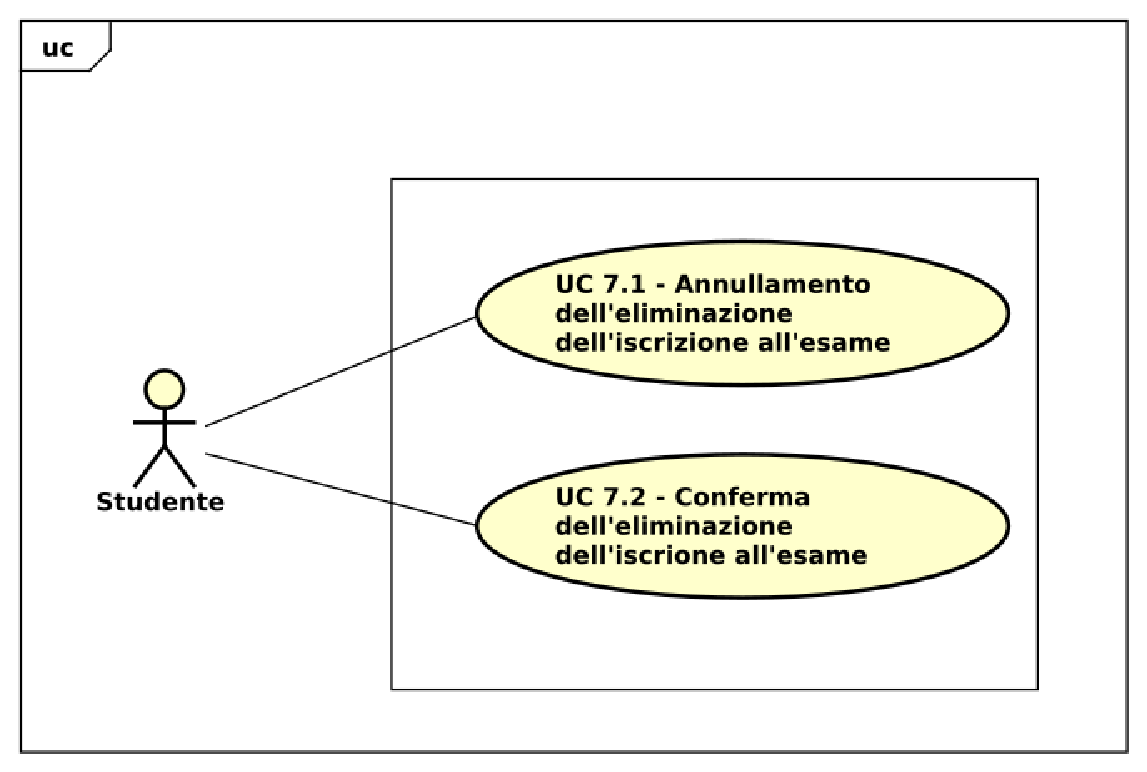
\includegraphics[scale=0.45]{./img/UC7.pdf}
	\caption{Eliminazione dell'iscrizione ad un esame}\label{}
\end{figure}
\begin{itemize}
	\item \textbf{Attori}: Studente;
	\item \textbf{Descrizione}: L'attore si è precedentemente iscritto ad un esame e può annullarne l'iscrizione;
	\item \textbf{Precondizione}: Il sistema fa visualizzare all'attore l'esame a cui esso è registrato;
	\item \textbf{Flusso principale degli eventi}: L'attore vuole eliminare l'iscrizione ad un esame a cui si è precedentemente registrato e può fare due scelte:
	\begin{itemize}
		\item Annullamento dell'eliminazione dell'iscrizione ad un esame (UC7.1);
		\item Conferma dell'eliminazione dell'iscrizione ad un esame (UC7.2).
	\end{itemize}
	\item \textbf{Postcondizione}: Il sistema disiscrive l'attore a quell'esame.
\end{itemize}
\subsection{Caso d'uso \texorpdfstring{UC7.1}{UC7.1}: Annullamento dell'eliminazione dell'iscrizione ad un esame}
\begin{itemize}
	\item \textbf{Attori}: Studente;
	\item \textbf{Descrizione}: L'attore sta eliminando l'iscrizione ad un esame ma decide di non farlo;
	\item \textbf{Precondizione}: Il sistema fa visualizzare all'attore l'esame a cui esso è registrato;
	
	\item \textbf{Flusso principale degli eventi}: L'attore che sta eliminando l'iscrizione ad un esame decide di annullare l'operazione;
	\item \textbf{Postcondizione}: Il sistema non disiscrive più l'attore a quell'esame in quanto esso ha annullato l'operazione.
	
\end{itemize}
\subsection{Caso d'uso \texorpdfstring{UC7.2}{UC7.2}: Conferma dell'eliminazione dell'iscrizione ad un esame}
\begin{itemize}
	\item \textbf{Attori}: Studente;
	\item \textbf{Descrizione}: L'attore che sta eliminando l'iscrizione ad un esame conferma tale scelta;
	\item \textbf{Precondizione}: Il sistema fa visualizzare all'attore l'esame a cui esso vuole disiscriversi;
	
	\item \textbf{Flusso principale degli eventi}: L'attore conferma l'eliminazione di un'iscrizione ad un esame;
	\item \textbf{Postcondizione}: Il sistema disiscrive l'attore a quell'esame.
	
\end{itemize}
\subsection{Caso d'uso \texorpdfstring{UC8}{UC8}: Rifiuto del voto di un esame}
\begin{itemize}
	\item \textbf{Attori}: Studente;
	\item \textbf{Descrizione}: L'attore può rifiutare il voto di un esame;
	\item \textbf{Precondizione}: Il sistema fa visualizzare all'attore il voto relativo ad esame che esso ha sostenuto;
	\item \textbf{Flusso principale degli eventi}: L'attore dopo aver visualizzato il voto dell'esame decide di rifiutarne il voto;
	\item \textbf{Postcondizione}: Il sistema non mostra alcun voto relativo a quell'esame in quanto l'attore l'ha rifiutato.
\end{itemize}
\subsection{Caso d'uso \texorpdfstring{UC9}{UC9}: Modifica di un esame da parte di un professore}
\begin{figure} [H]
	\centering
	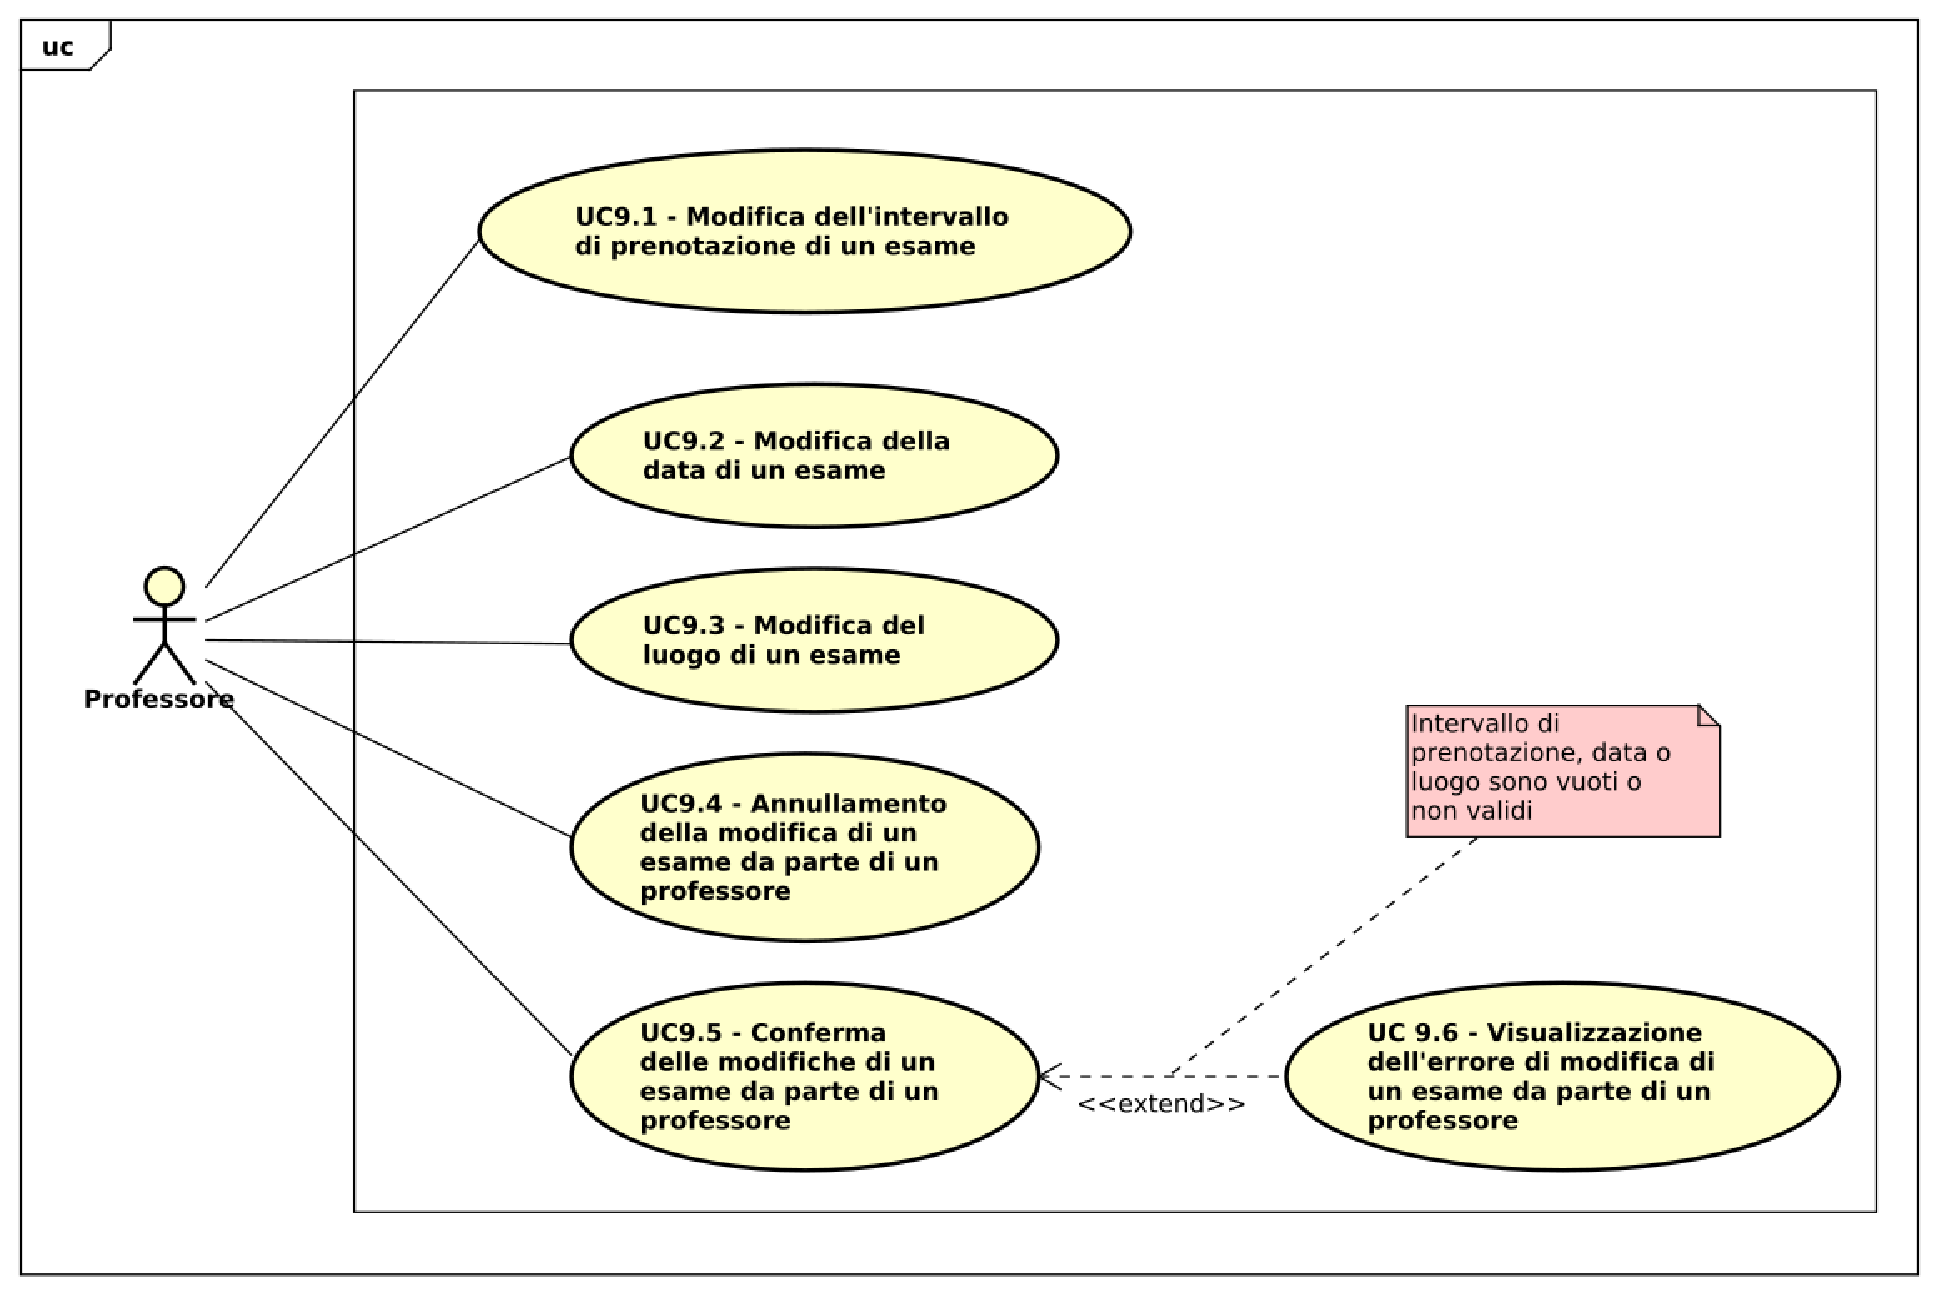
\includegraphics[scale=0.45]{./img/UC9.pdf}
	\caption{Modifica di un esame da parte di un professore}\label{}
\end{figure}
\begin{itemize}
	\item \textbf{Attori}: Professore;
	\item \textbf{Descrizione}: L'attore ha accesso alla modifica di alcuni campi dati degli esami a cui sono assegnati;
	\item \textbf{Precondizione}: Il sistema fa visualizzare un esame al professore;
	
	\item \textbf{Flusso principale degli eventi}: L'attore ha possibilità di modifica dei seguenti punti degli esami a cui è assegnato:
	\begin{itemize}
		\item Modifica dell'intervallo di prenotazione di un esame (UC9.1);
		\item Modifica della data di un esame (UC9.2);
		\item Modifica del luogo di un esame (UC9.3);
		\item Annullamento della modifica di un esame da parte di un professore (UC9.4);
		\item Conferma della modifica di un esame da parte di un professore (UC9.5);
		\item Visualizzazione dell'errore di modifica di un esame da parte di un professore (UC9.6).
	\end{itemize}
	\item \textbf{Postcondizione}: Il sistema ha modificato l'esame in quanto il professore ha attuato l'operazione di modifica.
	
\end{itemize}
\subsection{Caso d'uso \texorpdfstring{UC9.1}{UC9.1}: Modifica dell'intervallo di prenotazione di un esame}
\begin{itemize}
	\item \textbf{Attori}: Professore;
	\item \textbf{Descrizione}: L'attore modifica l'intervallo temporale per cui uno studente ha la possibilità di iscriversi ad un esame;
	\item \textbf{Precondizione}: Il sistema fa visualizzare un esame al professore;
	
	
	\item \textbf{Flusso principale degli eventi}: L'attore modifica l'intervallo di prenotazione di un esame;
	\item \textbf{Postcondizione}: Il sistema ha modificato l'intervallo di prenotazione per l’esame in quanto il professore ha attuato l'operazione di modifica.
	
\end{itemize}
\subsection{Caso d'uso \texorpdfstring{UC9.2}{UC9.2}: Modifica della data di un esame}
\begin{itemize}
	\item \textbf{Attori}: Professore;
	\item \textbf{Descrizione}: L'attore ha la possibilità di modificare la data di un esame;
	\item \textbf{Precondizione}: Il sistema fa visualizzare un esame al professore;
	
	\item \textbf{Flusso principale degli eventi}: L'attore modifica la data di un esame;
	\item \textbf{Postcondizione}: Il sistema ha modificato l'intervallo di prenotazione per l’esame in quanto il professore ha attuato l'operazione di modifica.
	
\end{itemize}
\subsection{Caso d'uso \texorpdfstring{UC9.3}{UC9.3}: Modifica del luogo di un esame}
\begin{itemize}
	\item \textbf{Attori}: Professore;
	\item \textbf{Descrizione}: L'attore ha la possibilità di modificare il luogo degli esami a cui è assegnato;
	\item \textbf{Precondizione}: Il sistema fa visualizzare un esame al professore;
	
	\item \textbf{Flusso principale degli eventi}: L'attore modifica il luogo di un esame;
	\item \textbf{Postcondizione}: Il sistema ha modificato il luogo dell'esame in quanto il professore ha attuato l'operazione di modifica.
	
\end{itemize}
\subsection{Caso d'uso \texorpdfstring{UC9.4}{UC9.4}: Annullamento della modifica di un esame da parte di un professore}
\begin{itemize}
	\item \textbf{Attori}: Professore;
	\item \textbf{Descrizione}: L'attore che sta modificando un esame decide di annullare l'operazione;
	\item \textbf{Precondizione}: Il sistema fa visualizzare al professore la pagina relativa alla modifica di un esame;
	
	\item \textbf{Flusso principale degli eventi}: L'attore annulla le modifiche che sta compiendo;
	\item \textbf{Postcondizione}: Il sistema non modifica più un esame in quanto il professore ha annullato l'operazione.
	
\end{itemize}
\subsection{Caso d'uso \texorpdfstring{UC9.5}{UC9.5}: Conferma della modifica di un esame da parte di un professore}
\begin{itemize}
	\item \textbf{Attori}: Professore;
	\item \textbf{Descrizione}: L'attore che sta modificando un esame decide di confermare le modifiche;
	\item \textbf{Precondizione}: Il sistema fa visualizzare al professore la pagina relativa alla modifica di un esame;
	
	\item \textbf{Flusso principale degli eventi}: L'attore conferma le modifiche fatte all'esame;
	\item \textbf{Postcondizione}: Il sistema modifica un esame in quanto il professore ha confermato l'operazione;
	
	\item \textbf{Estensioni}:
	\begin{itemize}
		\item Visualizzazione dell'errore di modifica di un esame da parte di un professore (UC9.6).
	\end{itemize}
\end{itemize}
\subsection{Caso d'uso \texorpdfstring{UC9.6}{UC9.6}: Visualizzazione dell'errore di modifica di un esame da parte di un professore}
\begin{itemize}
	\item \textbf{Attori}: Professore;
	\item \textbf{Descrizione}: Il sistema visualizza un errore riguardante l'errata modifica dei campi dati di un esame;
	\item \textbf{Precondizione}: Il sistema ha ricevuto campi dati errati o vuoti da parte di un professore;
	
	\item \textbf{Flusso principale degli eventi}: L'attore, modificando in maniera errata i campi dell'esame, può visualizzare uno dei seguenti errori: \begin{itemize}
		\item Intervallo di prenotazione per l’esame non valido o lasciato vuoto;
		\item Data dell’esame non valida o lasciato vuoto;
		\item Luogo d’esame non valido o lasciato vuoto.
	\end{itemize}
	\item \textbf{Postcondizione}: Il sistema fa visualizzare al professore un messaggio d'errore relativo all'operazione di modifica di un esame
	
\end{itemize}
\subsection{Caso d'uso \texorpdfstring{UC10}{UC10}: Inserimento di un voto }
\begin{figure} [H]
	\centering
	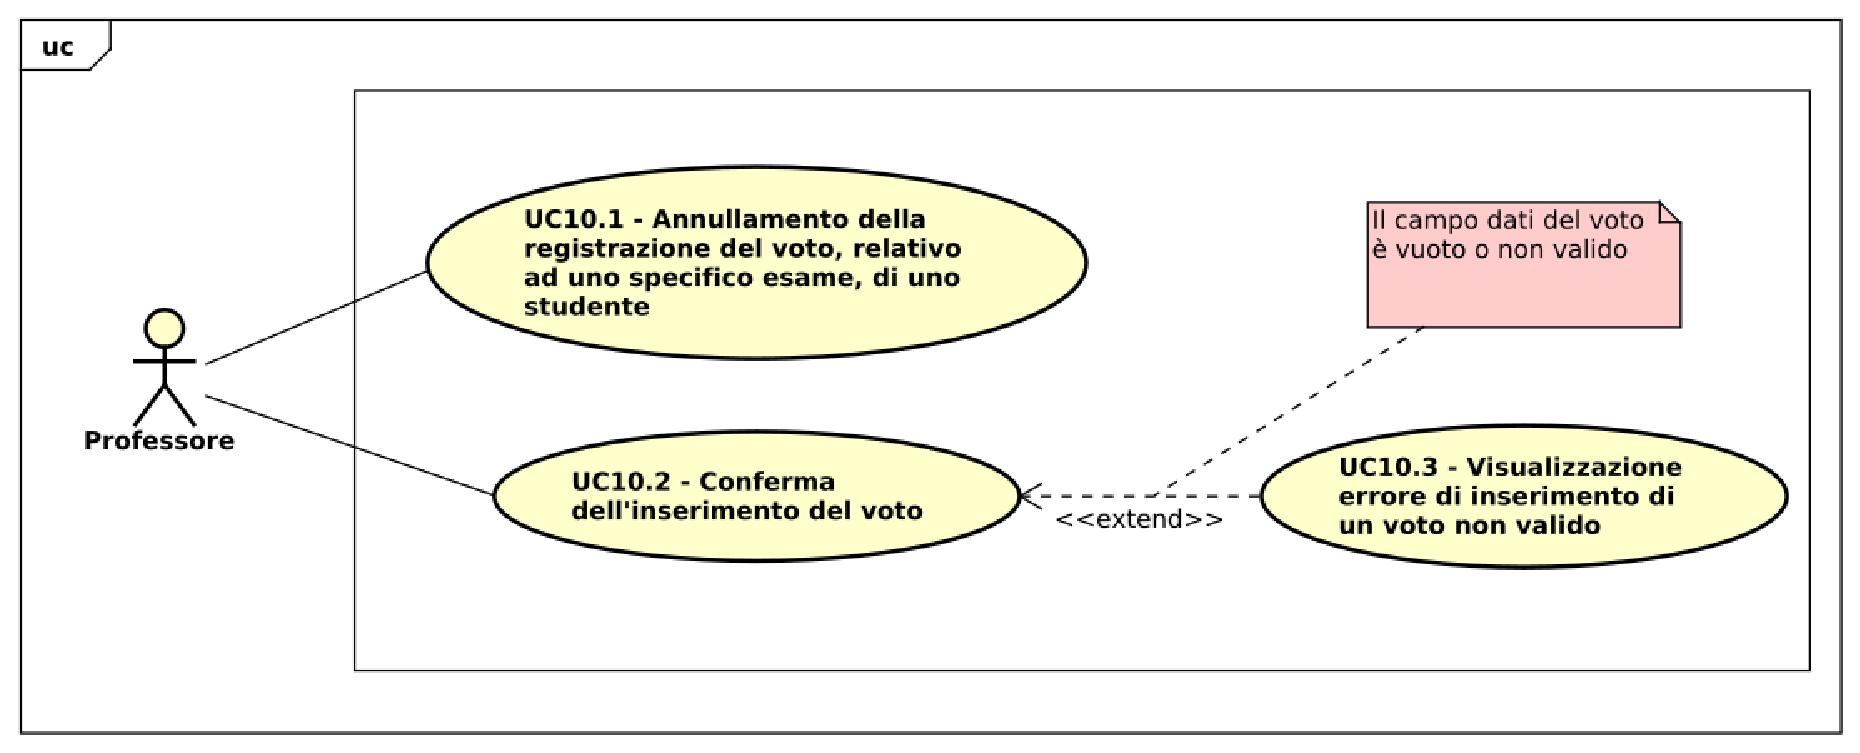
\includegraphics[scale=0.45]{./img/UC10.pdf}
	\caption{Inserimento di un voto }\label{}
\end{figure}
\begin{itemize}
	\item \textbf{Attori}: Professore;
	\item \textbf{Descrizione}: L'attore visualizza la lista degli studenti iscritti all'esame e assegna una votazione;
	\item \textbf{Precondizione}: Il sistema fa visualizzare all'attore la lista degli studenti iscritti all'esame;
	\item \textbf{Flusso principale degli eventi}: L'attore inserendo un voto ad uno studente si trova davanti ai seguenti scenari;
	\begin{itemize}
		\item Annullamento della registrazione del voto, relativo ad uno specifico esame, di uno studente (UC10.1);
		\item Conferma dell'inserimento di un voto (UC10.2);
		\item Visualizzazione dell'errore di inserimento di un voto non valido (UC10.3).
	\end{itemize}
	\item \textbf{Postcondizione}: Il sistema fa visualizzare il campo, che può essere stato compilato, relativo al voto di uno studente per un esame.
\end{itemize}
\subsection{Caso d'uso \texorpdfstring{UC10.1}{UC10.1}: Annullamento della registrazione del voto, relativo ad uno specifico esame, di uno studente}
\begin{itemize}
	\item \textbf{Attori}: Professore;
	\item \textbf{Descrizione}: L'attore sta inserendo il voto ad uno studente e decide di annullare l'operazione;
	\item \textbf{Precondizione}: Il sistema fa visualizzare all'attore la lista degli studenti iscritti all'esame;
	
	\item \textbf{Flusso principale degli eventi}: L'attore che sta inserendo un voto può decidere di annullare l'operazione;
	\item \textbf{Postcondizione}: Il sistema non inserisce più il voto allo studente in quanto l'attore ha annullato l'operazione.
	
\end{itemize}
\subsection{Caso d'uso \texorpdfstring{UC10.2}{UC10.2}: Conferma dell'inserimento di un voto}
\begin{itemize}
	\item \textbf{Attori}: Professore;
	\item \textbf{Descrizione}: L'attore dopo aver immesso il voto dello studete decide di confermarlo;
	\item \textbf{Precondizione}: Il sistema fa visualizzare il campo, che può essere stato compilato, relativo al voto di uno studente per un esame;
	\item \textbf{Flusso principale degli eventi}: L'attore che inserisce il voto allo studente può confermarlo;
	\item \textbf{Postcondizione}: Il sistema inserisce il voto allo studente in quanto l'attore ha confermato l'operazione.
	\item \textbf{Estensioni}:
	\begin{itemize}
		\item Visualizzazione dell'errore di inserimento di un voto non valido (UC10.3).
	\end{itemize}
\end{itemize}
\subsection{Caso d'uso \texorpdfstring{UC10.3}{UC10.3}: Visualizzazione dell'errore di inserimento di un voto non valido}
\begin{itemize}
	\item \textbf{Attori}: Professore;
	\item \textbf{Descrizione}: Il sistema visualizza un messaggio di errore causato dall'immissione di un voto non conforme;
	\item \textbf{Precondizione}: Il sistema ha ricevuto un voto non valido;
	
	\item \textbf{Flusso principale degli eventi}: L'attore, che sbaglia ad inserire un voto, visualizza un messaggio d'errore relativo ad esso;
	\item \textbf{Postcondizione}: Il sistema fa visualizzare un messaggio d'errore riguardante il tentativo di inserire un voto non valido.
\end{itemize}
\subsection{Caso d'uso \texorpdfstring{UC11}{UC11}: Inserimento di un utente nel sistema}
\begin{figure} [H]
	\centering
	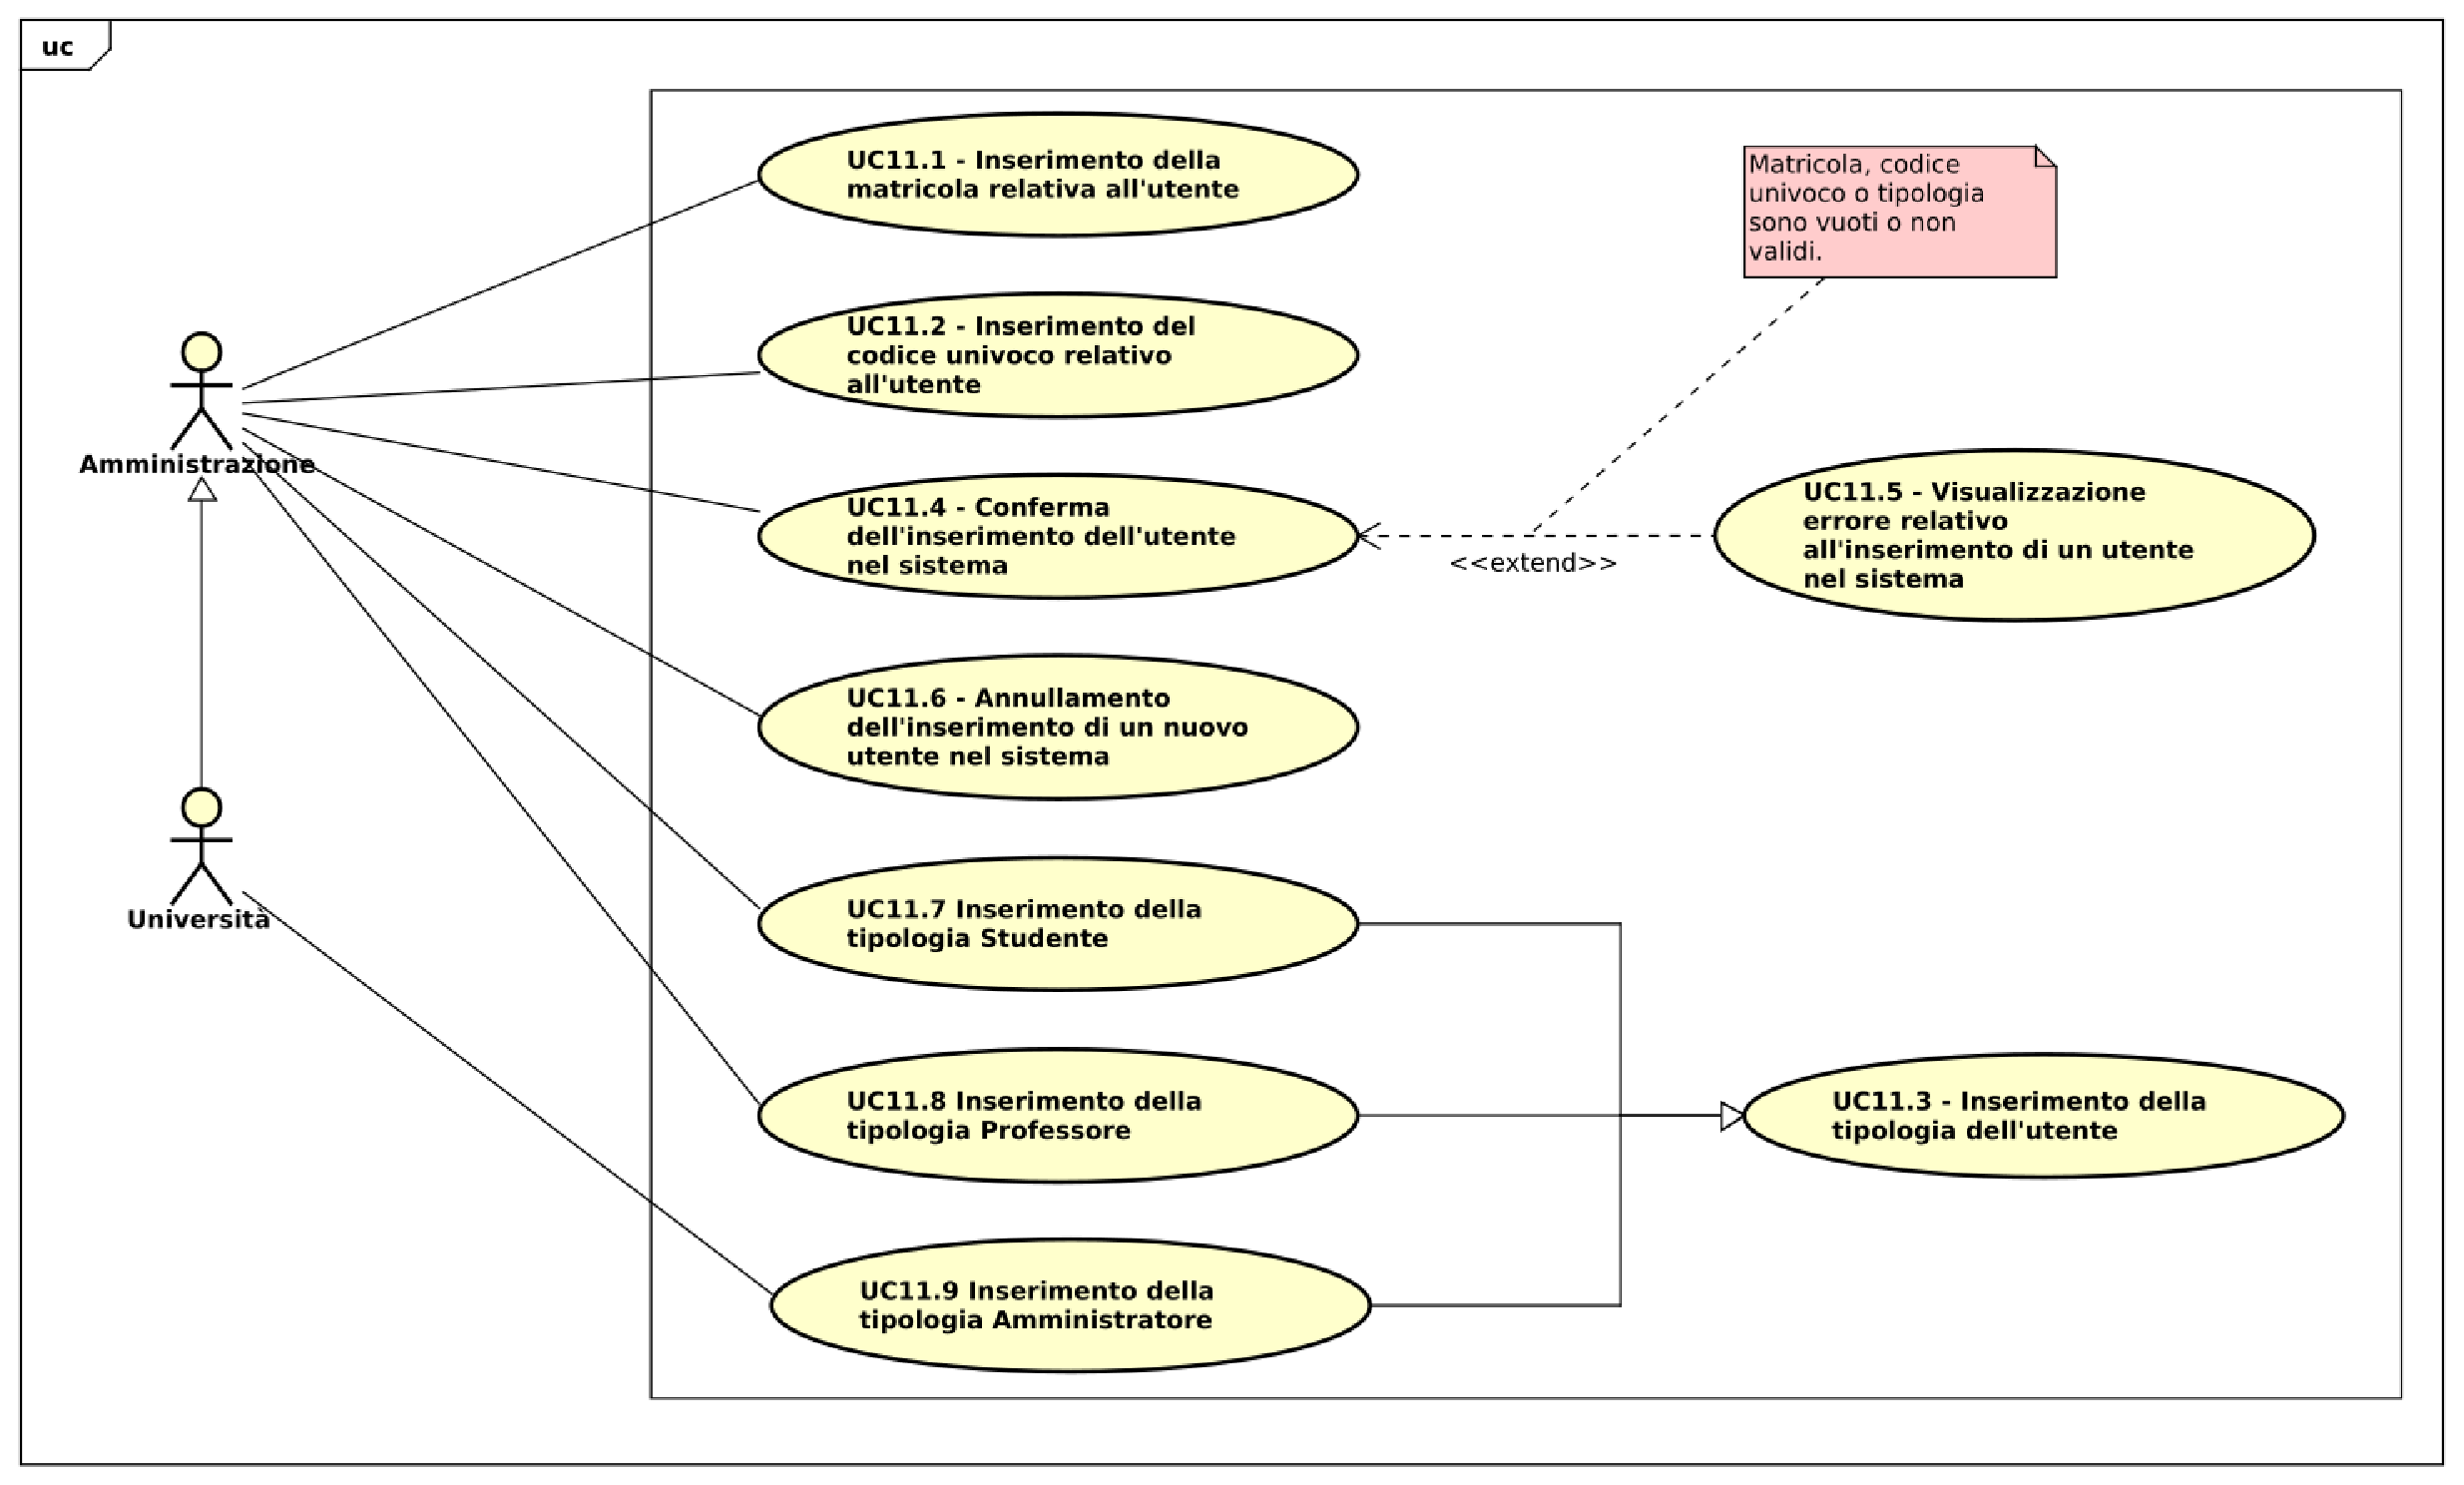
\includegraphics[scale=0.45]{./img/UC11.pdf}
	\caption{Inserimento di un utente nel sistema}\label{}
\end{figure}
\begin{itemize}
	\item \textbf{Attori}: Amministratore, Università;
	\item \textbf{Descrizione}: L'attore può inserire un nuovo utente nel sistema;
	\item \textbf{Precondizione}: Il sistema è pronto per inserire un nuovo utente;
	\item \textbf{Flusso principale degli eventi}: L'attore può inserire un nuovo utente nel sistema, che non sia già presente in esso, seguendo i seguenti passi:
	\begin{itemize}
		\item Inserimento della matricola relativa ad un utente (UC11.1);
		\item Inserimento del codice univoco relativo ad un utente (UC11.2);
		\item Inserimento della tipologia di un utente  (UC11.3);
		\item Conferma dell'inserimento di un utente nel sistema (UC11.4);
		\item Visualizzazione dell'errore relativo all'inserimento di un utente nel sistema (UC11.5);
		\item Annullamento dell'inserimento di un nuovo utente nel sistema (UC11.6);
		\item Inserimento della tipologia Studente (UC11.7);
		\item Inserimento della tipologia Professore (UC11.8);
		\item Inserimento della tipologia Amministratore (UC11.9).
	\end{itemize}
	\item \textbf{Postcondizione}: Il sistema può aver compilato dei campi relativi all'inserimento di un utente nel sistema.
	
\end{itemize}
\subsection{Caso d'uso \texorpdfstring{UC11.1}{UC11.1}: Inserimento della matricola relativa ad un utente}
\begin{itemize}
	\item \textbf{Attori}: Amministratore, Università;
	\item \textbf{Descrizione}: L'attore può inserire la matricola relativa all'utente;
	\item \textbf{Precondizione}: Il sistema fa visualizzare il campo della matricola relativa all'utente;
	\item \textbf{Flusso principale degli eventi}: L'attore può inserire la matricola dell'utente durante il suo inserimento nel sistema;
	\item \textbf{Postcondizione}: È stata inserita la matricola relativa all'utente nel campo opportuno.
\end{itemize}
\subsection{Caso d'uso \texorpdfstring{UC11.2}{UC11.2}: Inserimento del codice univoco relativo ad un utente}
\begin{itemize}
	\item \textbf{Attori}: Amministratore, Università;
	\item \textbf{Descrizione}: L'attore può inserire il codice univoco relativo all'utente;
	\item \textbf{Precondizione}: Il sistema fa visualizzare il campo del codice univoco relativo all'utente;
	
	\item \textbf{Flusso principale degli eventi}: L'attore può inserire il codice univoco dell'utente durante il suo inserimento nel sistema;
	\item \textbf{Postcondizione}: È stato inserito il codice univoco relativo all'utente nel campo opportuno.
	
\end{itemize}
\subsection{Caso d'uso \texorpdfstring{UC11.3}{UC11.3}: Inserimento della tipologia di un utente }
\begin{itemize}
	\item \textbf{Attori}: Amministratore, Università;
	\item \textbf{Descrizione}: L'attore può inserire la tipologia relativa all'utente;
	\item \textbf{Precondizione}: Il sistema fa visualizzare il campo della tipologia di un utente;
	
	\item \textbf{Flusso principale degli eventi}: L'attore può inserire la tipologia dell'utente;
	\item \textbf{Postcondizione}: È stata inserita la tipologia di un utente nel campo opportuno.
	
\end{itemize}
\subsection{Caso d'uso \texorpdfstring{UC11.4}{UC11.4}: Conferma dell'inserimento di un utente nel sistema}
\begin{itemize}
	\item \textbf{Attori}: Amministratore, Università;
	\item \textbf{Descrizione}: L'attore può confermare l'inserimento nel sistema;
	\item \textbf{Precondizione}: Il sistema fa visualizzare il campo, che può essere stato compilato, relativo all'inserimento di un utente nel sistema;
	\item \textbf{Flusso principale degli eventi}: L'attore può confermare l'inserimento dell'utente nel sistema;
	\item \textbf{Postcondizione}: Il sistema inserisce un nuovo utente in quanto l'attore ha confermato l'operazione.
	
	\item \textbf{Estensioni}:
	\begin{itemize}
		\item Visualizzazione dell'errore relativo all'inserimento di un utente nel sistema (UC11.5).
	\end{itemize}
\end{itemize}
\subsection{Caso d'uso \texorpdfstring{UC11.5}{UC11.5}: Visualizzazione dell'errore relativo all'inserimento di un utente nel sistema}
\begin{itemize}
	\item \textbf{Attori}: Amministratore, Università;
	\item \textbf{Descrizione}: L'attore aggiunge i dettagli relativi all'inserimento di un utente nel sistema senza rispettarne la validazione;
	\item \textbf{Precondizione}: Il sistema ha ricevuto campi dati errati o vuoti;
	
	
	\item \textbf{Flusso principale degli eventi}: L'attore, impostando in maniera errata i campi dell'utente, può visualizzare uno dei seguenti errori:
	\begin{itemize}
		\item Matricola non valida oppure lasciata vuota;
		\item Codice univoco non valido oppure lasciato vuoto.
	\end{itemize}
	\item \textbf{Postcondizione}: Il sistema fa visualizzare un messaggio d'errore riguardante il tentativo di inserire un nuovo utente.
	
\end{itemize}
\subsection{Caso d'uso \texorpdfstring{UC11.6}{UC11.6}: Annullamento dell'inserimento di un nuovo utente nel sistema}
\begin{itemize}
	\item \textbf{Attori}: Amministratore, Università;
	\item \textbf{Descrizione}: L'attore non inserisce più un nuovo utente nel sistema;
	\item \textbf{Precondizione}: l sistema fa visualizzare la pagina relativa all'inserimento di un nuovo utente nel sistema;
	
	\item \textbf{Flusso principale degli eventi}: L'attore non inserisce più un nuovo utente nel sistema e quindi annulla l'operazione;
	\item \textbf{Postcondizione}: Il sistema non aggiunge più un nuovo utente in quanto l'attore ha annullato l'operazione.
	
\end{itemize}
\subsection{Caso d'uso \texorpdfstring{UC11.7}{UC11.7}: Inserimento della tipologia Studente}
\begin{itemize}
	\item \textbf{Attori}: Amministratore, Università;
	\item \textbf{Descrizione}: L'attore ha scelto studente come tipologia di utente; 
	\item \textbf{Precondizione}: Il sistema permette la scelta della tipologia di utente;
	\item \textbf{Flusso principale degli eventi}: L'attore può scegliere quale tipologia di utente inserire;
	\item \textbf{Postcondizione}: Come tipologia di utente è stato scelto lo studente;
\end{itemize}
\subsection{Caso d'uso \texorpdfstring{UC11.8}{UC11.8}: Inserimento della tipologia Professore}
\begin{itemize}
	\item \textbf{Attori}: Amministratore, Università;
	\item \textbf{Descrizione}: L'attore ha scelto professore come tipologia di utente; 
	\item \textbf{Precondizione}: Il sistema permette la scelta della tipologia di utente;
	\item \textbf{Flusso principale degli eventi}: L'attore può scegliere quale tipologia di utente inserire;
	\item \textbf{Postcondizione}: Come tipologia di utente è stato scelto il professore;
\end{itemize}
\subsection{Caso d'uso \texorpdfstring{UC11.9}{UC11.9}: Inserimento della tipologia Amministratore}
\begin{itemize}
	\item \textbf{Attori}: Università;
	\item \textbf{Descrizione}: L'attore ha scelto amministratore come tipologia di utente; 
	\item \textbf{Precondizione}: Il sistema permette la scelta della tipologia di utente;
	\item \textbf{Flusso principale degli eventi}: L'attore può scegliere quale tipologia di utente inserire;
	\item \textbf{Postcondizione}: Come tipologia di utente è stato scelto l'amministratore;
\end{itemize}
\subsection{Caso d'uso \texorpdfstring{UC12}{UC12}: Rimozione di un utente dal sistema}
\begin{figure} [H]
	\centering
	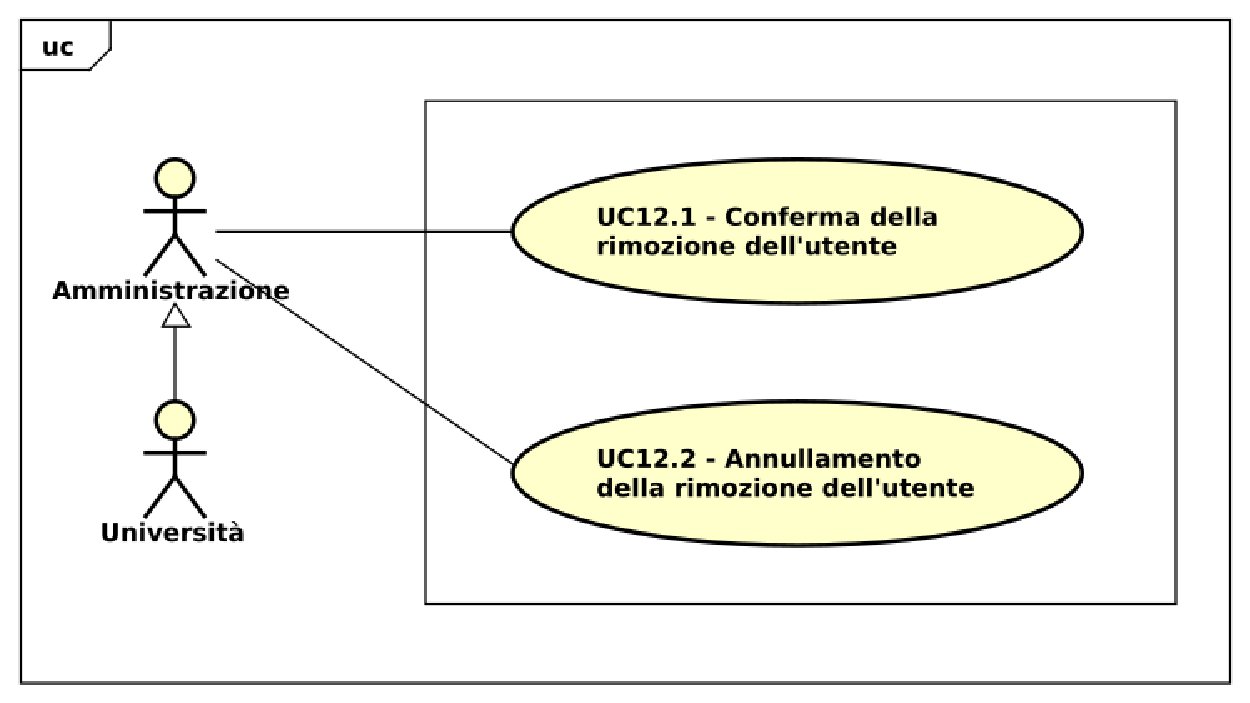
\includegraphics[scale=0.45]{./img/UC12.pdf}
	\caption{Rimozione di un utente dal sistema}\label{}
\end{figure}
\begin{itemize}
	\item \textbf{Attori}: Amministratore, Università;
	\item \textbf{Descrizione}: L'attore può rimuovere un utente, cancellandone tutti i dati ad esso associati nonché rimuovendone l'accesso al sistema;
	\item \textbf{Precondizione}: Il sistema riconosce come registrato l'utente che l'attore ha selezionato;
	\item \textbf{Flusso principale degli eventi}: L'attore, volendo rimuovere completamente un utente dal sistema, si troverà davanti alle seguenti scelte:
	\begin{itemize}
		\item Conferma della rimozione di un utente dal sistema (UC12.1);
		\item Annullamento della rimozione di un utente dal sistema (UC12.2).
	\end{itemize}
	\item \textbf{Postcondizione}: Il sistema fa visualizzare all'attore l'utente che ha selezionato per rimuoverlo dal sistema;
\end{itemize}
\subsection{Caso d'uso \texorpdfstring{UC12.1}{UC12.1}: Conferma della rimozione di un utente dal sistema}
\begin{itemize}
	\item \textbf{Attori}: Amministratore, Università;
	\item \textbf{Descrizione}: L'attore può confermare la rimozione di un utente dal sistema;
	\item \textbf{Precondizione}: Il sistema fa visualizzare all'attore l'utente che ha selezionato per rimuoverlo dal sistema;
	\item \textbf{Flusso principale degli eventi}: L'attore può confermare la rimozione di un utente dal sistema;
	\item \textbf{Postcondizione}: Il sistema ha cancellato la registrazione dell'utente nel sistema e tutti i suoi dati sono stati cancellati.
\end{itemize}
\subsection{Caso d'uso \texorpdfstring{UC12.2}{UC12.2}: Annullamento della rimozione di un utente dal sistema}
\begin{itemize}
	\item \textbf{Attori}: Amministratore, Università;
	\item \textbf{Descrizione}: L'attore può annullare la rimozione di un utente dal sistema;
	\item \textbf{Precondizione}: Il sistema fa visualizzare all'attore l'utente che ha selezionato per rimuoverlo dal sistema;
	
	\item \textbf{Flusso principale degli eventi}: L'attore può annullare l'azione di rimozione di un utente dal sistema;
	\item \textbf{Postcondizione}: Il sistema non cancella più la registrazione dell'utente nel sistema in quanto l'attore ha annullato l'operazione.
	
\end{itemize}
\subsection{Caso d'uso \texorpdfstring{UC13}{UC13}: Visualizzazione dell'errore relativo all'eliminazione di un anno accademico}
\begin{itemize}
	\item \textbf{Attori}: Amministratore, Università;
	\item \textbf{Descrizione}: Il sistema visualizza un messaggio d'errore riguardante l'impossibilità di eliminazione di un anno accademico;
	\item \textbf{Precondizione}: Il sistema fa visualizzare uno specifico anno accademico in corso;
	\item \textbf{Flusso principale degli eventi}: L'attore cercando di eliminare l'anno accademico in corso visualizza un messaggio d'errore;
	\item \textbf{Postcondizione}: Il sistema fa visualizzare un messaggio d'errore riguardante l'impossibilità di eliminazione di un anno accademico.
	
\end{itemize}
\subsection{Caso d'uso \texorpdfstring{UC14}{UC14}: Visualizzazione del libretto}
\begin{itemize}
	\item \textbf{Attori}: Studente;
	\item \textbf{Descrizione}: L'attore può visualizzare la lista di tutti gli esami ha sostenuto o dovrà sostenere;
	\item \textbf{Precondizione}: Il sistema ha registrati uno o più studenti;
	\item \textbf{Flusso principale degli eventi}: L'attore può visualizzare il suo libretto;
	\item \textbf{Postcondizione}: Il sistema fa visualizzare all'attore la lista degli esami sostenuti o che esso dovrà sostenere, che è il libretto.
\end{itemize}
\subsection{Caso d'uso \texorpdfstring{UC15}{UC15}: Visualizzazione degli esami associati}
\begin{itemize}
	\item \textbf{Attori}: Professore;
	\item \textbf{Descrizione}: L'attore può visualizzare la lista di tutti gli esami ad esso associati;
	\item \textbf{Precondizione}: Il sistema ha registrati uno o più professori;
	\item \textbf{Flusso principale degli eventi}: L'attore può visualizzare tutti gli esami che gli sono associati;
	\item \textbf{Postcondizione}: Il sistema fa visualizzare tutti gli esami associati all'attore.
\end{itemize}
\subsection{Caso d'uso \texorpdfstring{UC16}{UC16}: Visualizzazione degli studenti iscritti ad un esame associato}
\begin{itemize}
	\item \textbf{Attori}: Professore;
	\item \textbf{Descrizione}: L'attore può visualizzare tutti gli studenti che sono iscritti ad un esame a lui associato;
	\item \textbf{Precondizione}: Il sistema ha registrati uno o più professori e uno o più esami ad essi associati;
	\item \textbf{Flusso principale degli eventi}: L'attore può visualizzare la lista degli studenti che si sono iscritti ad un esame a lui associato;
	\item \textbf{Postcondizione}: Il sistema fa visualizzare una lista di studenti che sono iscritti ad un'esame associato all'attore.
\end{itemize}
